%\documentclass[lettersize,journal]{IEEEtran}
\documentclass[letterpaper, 10 pt, journal, twoside]{IEEEtran}
\usepackage{amsmath,amsfonts}
%\usepackage{algorithmic}
%\usepackage{algorithm}
\usepackage{array}
\usepackage[caption=false,font=normalsize,labelfont=sf,textfont=sf]{subfig}
\usepackage{textcomp}
\usepackage{stfloats}
\usepackage{url}
\usepackage{verbatim}
\usepackage{graphicx}
%\usepackage{boondox-cal}
%\usepackage{cite}
\usepackage[linesnumbered,ruled,vlined]{algorithm2e}%[ruled,vlined]{  
\usepackage{algcompatible}
%\usepackage{svg}
\usepackage{makecell}
\usepackage[backend=bibtex]{biblatex} %\usepackage{ulem}
\usepackage{color}
\usepackage{ulem}
\usepackage{pifont}
\usepackage[export]{adjustbox}
\usepackage{soul, color, xcolor}

\usepackage[colorlinks,
            linkcolor=blue,
            anchorcolor=blue,
            citecolor=blue]{hyperref}
            
\newtheorem{myDef}{Definition}
\newtheorem{myTheo}{Theorem}
\newtheorem{myProof}{Proof}
\newtheorem{myLemma}{Lemma}

\bibliography{mybibfile}

\begin{document}


\title{An efficient tangent graph-based path planning for multiple topologically distinctive paths}

\author{Zhuo Yao, Wei Wang$\ast$
\thanks{Corresponding by Wei Wang: wangweilab@buaa.edu.cn.
This work was supported by the National Key Research and Development Program of China under grant number 2020YFB1313600.}
}

% The paper headers
\markboth{Journal of \LaTeX\ Class Files,~Vol.~14, No.~8, August~2021}%
{Shell \MakeLowercase{\textit{et al.}}: A Sample Article Using IEEEtran.cls for IEEE Journals}

%\IEEEpubid{0000--0000/00\$00.00~\copyright~2021 IEEE}
% Remember, if you use this you must call \IEEEpubidadjcol in the second
% column for its text to clear the IEEEpubid mark.

\maketitle

\begin{abstract}

Classic conventional topologically distinctive path planning relies on indicators related to the number of isolated obstacles to determine whether two paths belong to the same topology. This reliance often hinders real-time processing (\textless 1s) in maps with numerous isolated obstacles. Furthermore, most existing topologically distinctive path planning methods require multiple graph searches to obtain multiple paths, resulting in non-real-time performance when searching for hundreds of topologically distinctive paths. In light of these challenges, we propose an efficient path planning approach based on tangent graphs to discover multiple topologically distinctive paths. Our method diverges from existing algorithms by eliminating the need to distinguish whether two paths belong to the same topology. Instead, it generates multiple topologically distinctive paths based on the locally shortest property of tangents. Additionally, we introduce an expansion reduction mechanism for the queue during graph search, thereby preventing the exponential expansion of the queue size. To illustrate the advantages of our method, we conducted a comparative analysis with various typical algorithms using a widely recognized public dataset. The results indicate that, on average, our method generates 400 topologically distinctive paths within 250 milliseconds. This outcome underscores a significant enhancement in efficiency compared to existing methods. 


\end{abstract}

\begin{IEEEkeywords}
distinctive topology path, tangent graph, trajectory optimization, path planning.
\end{IEEEkeywords}

\section{Introduction}


Topology of paths/trajectories arises due to the presence of obstacles in an environment. Two paths/trajectories connecting the same start and goal coordinates are in the same homotopy class if they can be smoothly deformed into one another without intersecting any obstacles in the environment; otherwise, they are in different topology classes.

In many applications of robots and MAVs, it is crucial to get multiple topologically distinctive paths. In exploring unknown space, \cite{kim2013topological} uses topologically distinctive paths to deploy a group of agents to explore an environment (e.g., for eliminating potential threats, searching for rewards/targets, as well as for updating the obstacle map of a partially known environment). \cite{kim2021topology} developed a perception-aware planner that selects the path with the highest perception quality from a set of multiple topologically distinctive paths for MAVs. In social robots, Palmieri et al. \cite{palmieri2015fast} used a topologically distinctive path planning (also known as topology-aware path planning) method to find multiple socially-aware paths. In motion planning, \cite{kuderer2014online} uses a set of topologically distinctive paths to overcome such local minima and to quickly propose a set of alternative, topologically different, and optimized paths. \cite{rosmann2017integrated} maintains and simultaneously optimizes a subset of admissible candidate trajectories of distinctive topologies, thus seeking the overall best candidate among the set of alternative local solutions. \cite{li2022online} proposed an online trajectory replanning method that using homotopic distinctive path for better trajectoryfor automated parking. \cite{kolur2019online} selects topologically distinctive paths in automated driving's trajectory planning to find the optimal maneuver in scenarios with multiple obstacles. 


\begin{figure}[t] \scriptsize
%\begin{tabular}{cc}
\begin{minipage}{.48\linewidth}
  \centerline{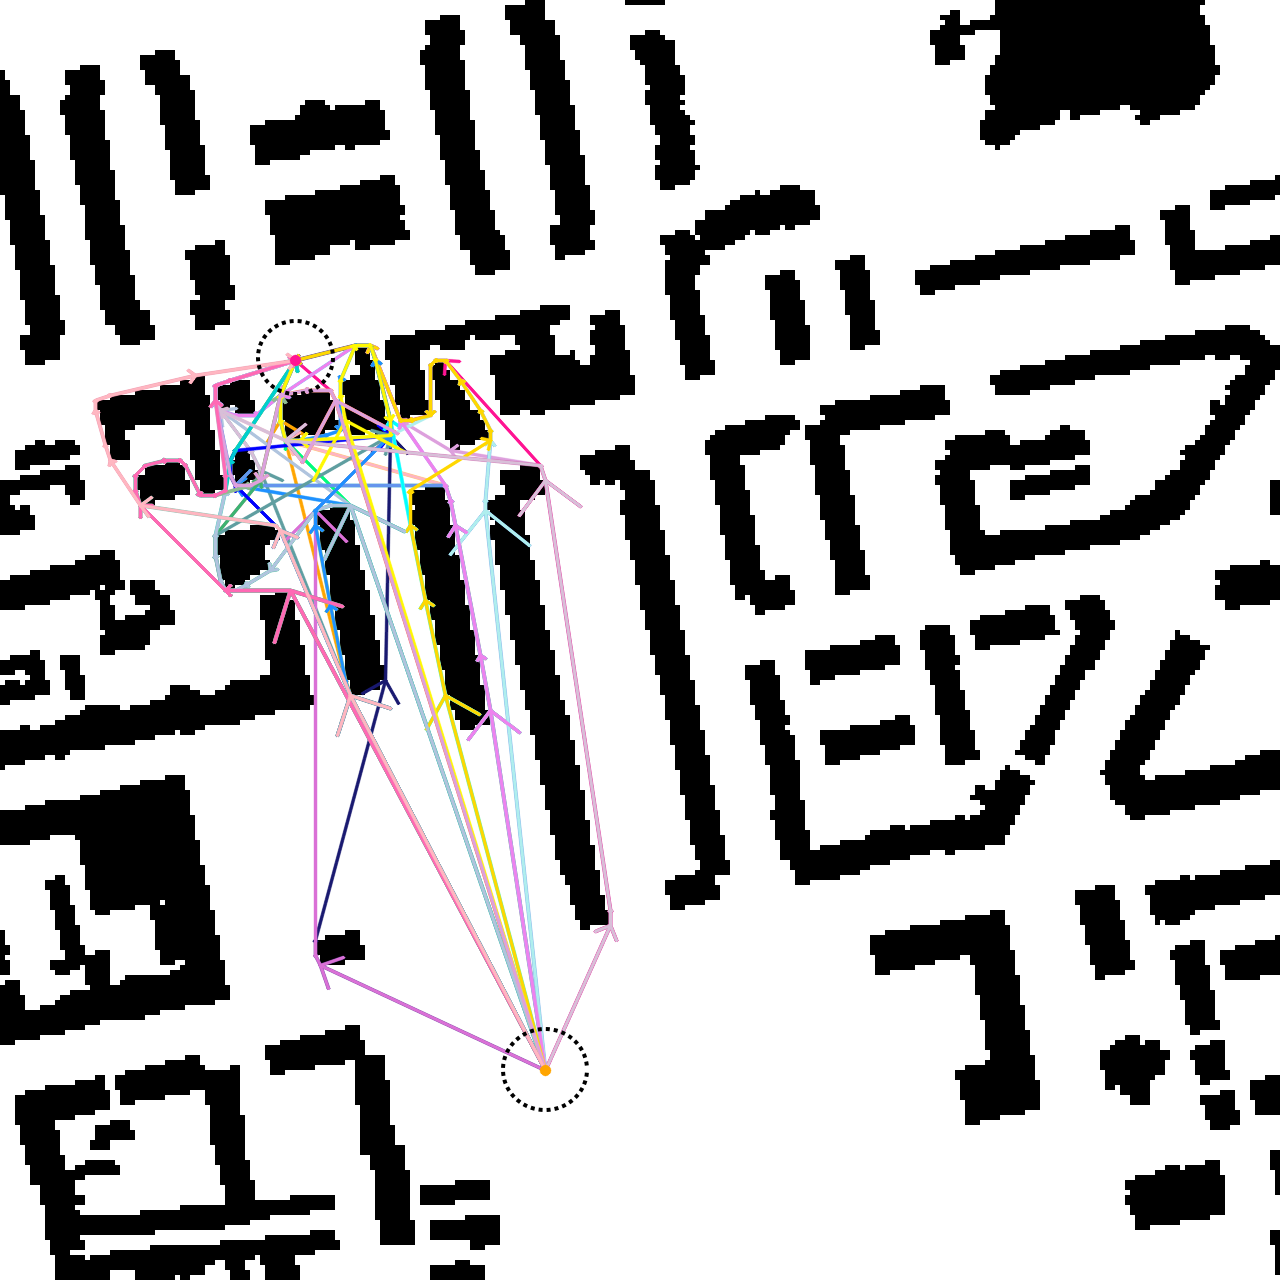
\includegraphics[width=4.2cm, cframe=gray .2mm]{50_RJ.png}}
  \centerline{A: 50 paths, in 3.7ms}
\end{minipage}
\hfill
\begin{minipage}{.48\linewidth}
  \centerline{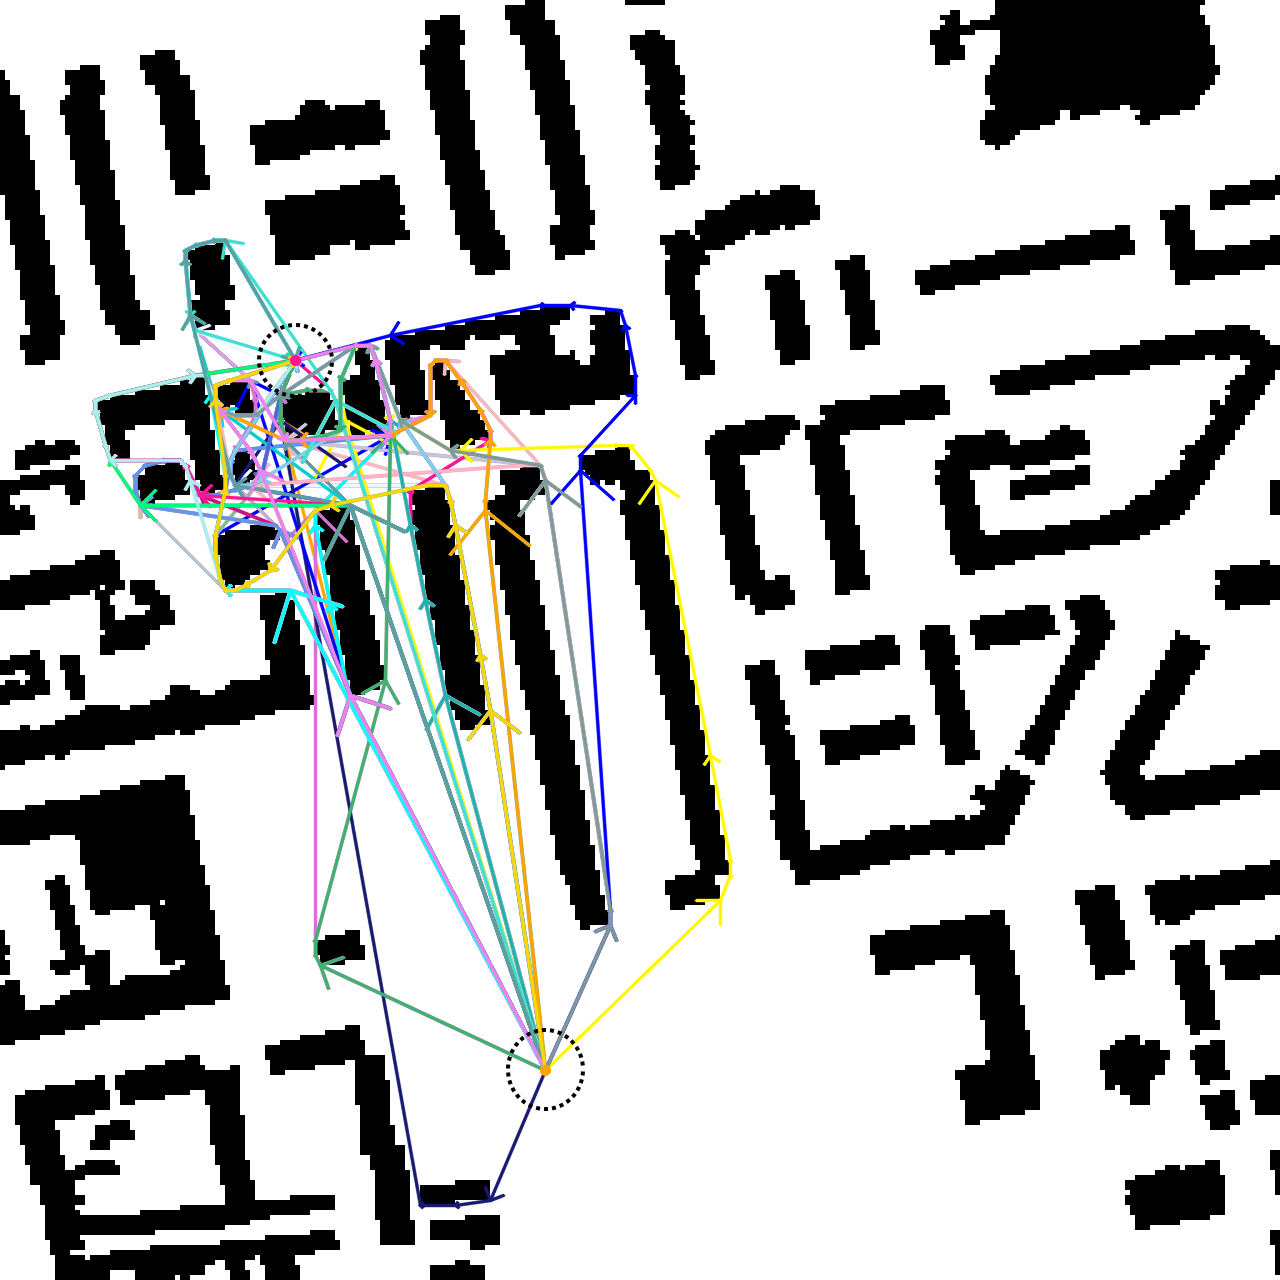
\includegraphics[width=4.2cm, cframe=gray 0.1mm]{100_RJ.png}}
  \centerline{B: 100 paths, in 8.2ms}
\end{minipage}
\vfill
\begin{minipage}{.48\linewidth}
  \centerline{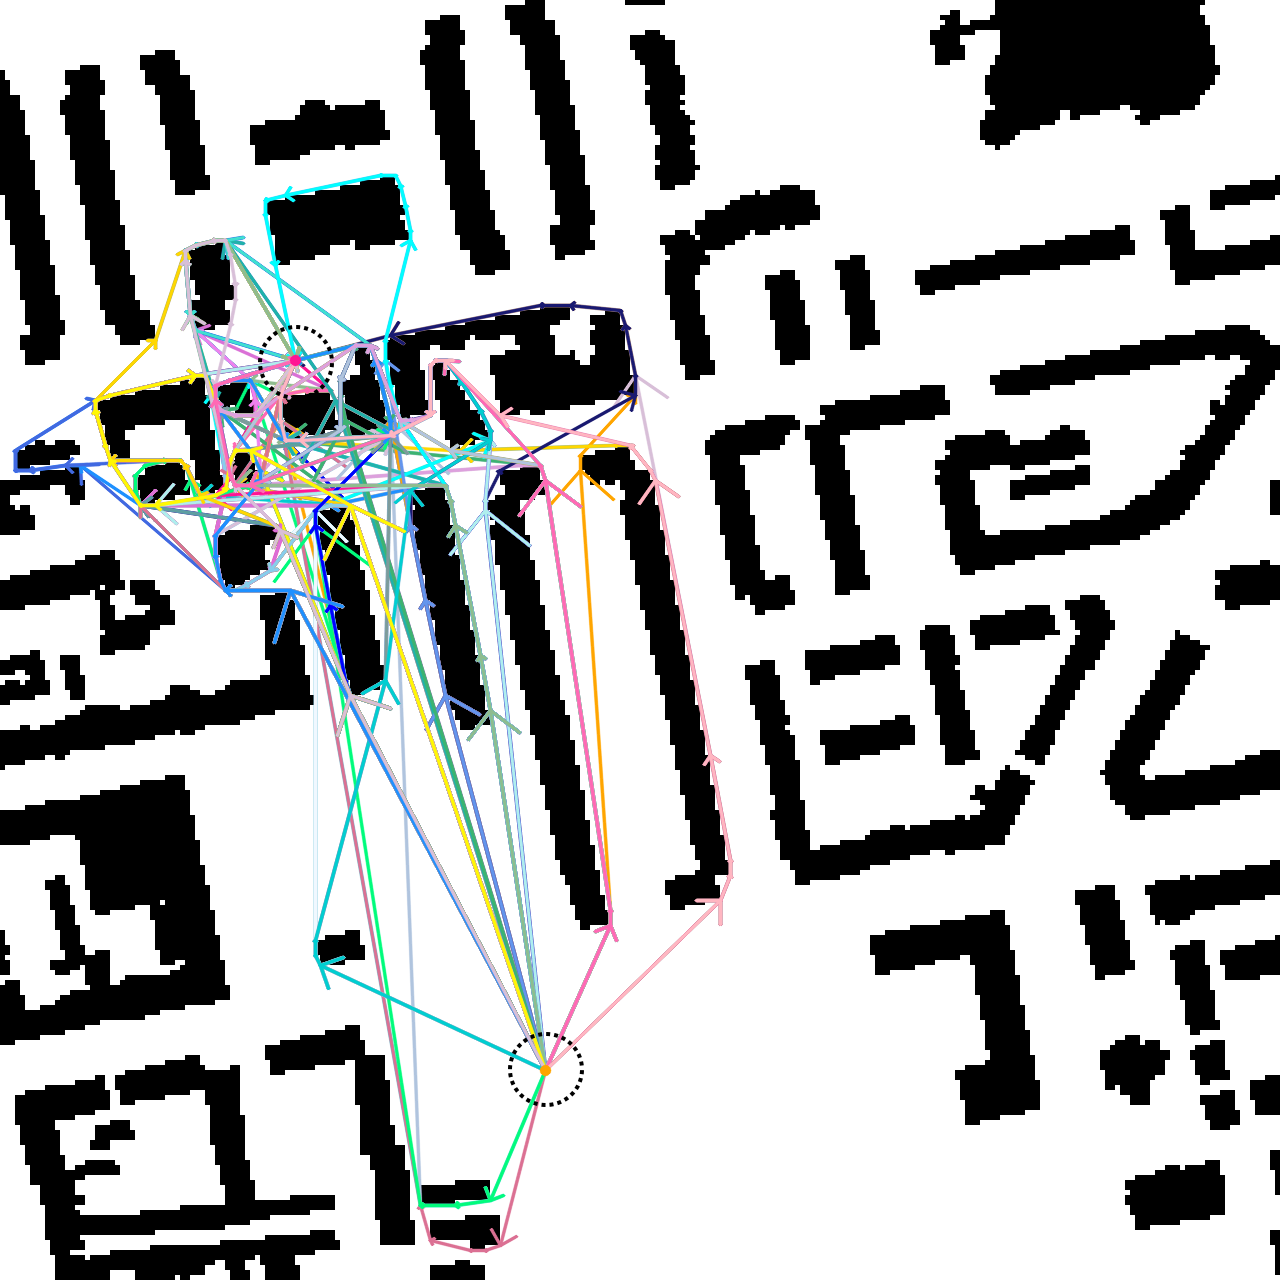
\includegraphics[width=4.2cm, cframe=gray 0.1mm]{200_RJ.png}}
  \centerline{C: 200 paths, in 16.2ms}
\end{minipage}
\hfill
\begin{minipage}{.48\linewidth}
  \centerline{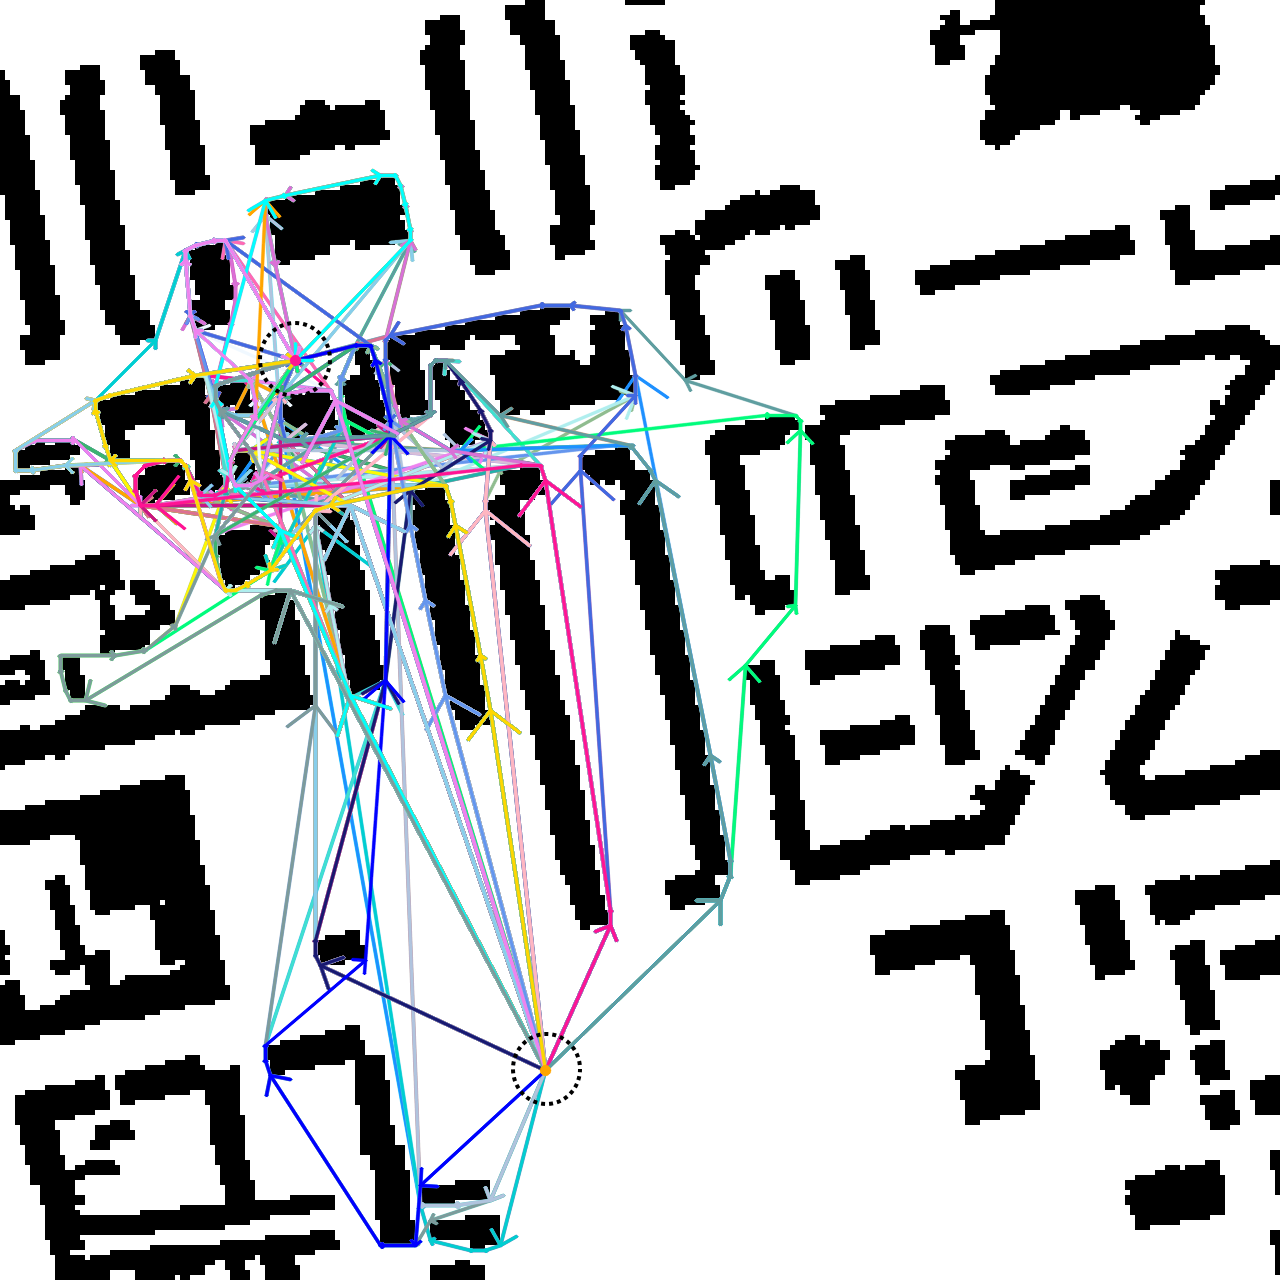
\includegraphics[width=4.2cm, cframe=gray 0.1mm]{400_RJ.png}}
  \centerline{D: 400 paths, in 38.1ms}
\end{minipage}
\vfill
\caption{These figures display multiple paths, with some of them partially overlapping, between the same start and target points, all determined by our method. The map employed is a 256x256 grid map ("Berlin\_1\_256" from the mentioned public map dataset). The start and target points, highlighted in pink and yellow, respectively, have coordinates (59, 72) and (109, 214), located at the center of circles. These experiments were conducted on a standard laptop running the Ubuntu operating system, equipped with a 3.2GHz CPU and 16GB of memory. Further details can be found in the Results section. }
\label{examples}
\end{figure}


Algorithms related to obtaining topologically distinctive paths have been researched for decades. However, several difficulties are encountered by existing works. Firstly, some of them require the use of indicators (e.g., H-signature \cite{2, 3}, string representation \cite{yi2017topology}) based on each isolated obstacle and its representative points to determine whether two paths belong to the same topology. Secondly, almost all of them need multiple times of search to get multiple paths, which resulted them are ineffective to search hundreds of path online.

Considering the criteria to score a path is variously under different scenarios, the more the number of topologically distinctive paths the more chance to get better paths. However, existing methods relay on multiple search to get multiple paths or using indicators that depends on each isolated obstacles, resulting them have poor performance to search hundereds of path or work under maps contain lots of isolated obstacles. Thus, it's significant to develop a more efficient and higher quality topologically distinctive path planning. Specificly, a method that search multiple paths in one search and do not need an explicit indicators which is time consuming under map with lots of obstacles.

To address the aforementioned drawbacks, we propose a novel algorithm for topologically distinctive path planning based on tangent graphs. Our method using  no an expilict indicators and avoids the repetition of graph searches to obtain multiple topologically distinctive paths. Additionally, we introduce an expansion reduction mechanism to prevent the exponential growth of the queue size during graph search.

The results demonstrate a remarkable enhancement in efficiency during the path planning process. A brief demonstration of our algorithm is presented in Fig. \ref{examples}.


%The following sections of this article are organized as follows: Section \ref{RelatedWork} offers an introduction to relevant studies on distinctive topology path planning; section \ref{Methodology} provides a detailed description of the theory basis and key processes involved in our method; in Section \ref{Results}, we delve into the details of the construction of the tangent graph on the specified maps. Additionally, we present a comprehensive comparison between our method and several typical methods in terms of time cost, success rate and path length. This section also includes information about how our method performs as the number of paths increases and the scale of map increases; finally, in Section \ref{Conclusion}, we discuss the results obtained and potential drawbacks of the proposed method.

The following sections of this article are organized as follows: Section \ref{RelatedWork} introduces relevant studies on distinctive topology path planning. Section \ref{Methodology} provides a detailed description of the theoretical basis and key processes involved in our method. In Section \ref{Results}, we delve into the details of constructing the tangent graph on specified maps. Additionally, we present a comprehensive comparison between our method and several typical methods in terms of time cost, success rate, and path length. This section also includes information about how our method performs as the number of paths increases and the scale of the map increases. Finally, in Section \ref{Conclusion}, we discuss the results obtained and potential drawbacks of the proposed method.

This article contributes the following:

\begin{enumerate}
    \item A new theory: "For 2D Euclidean space, each locally shortest path corresponds to a topologically unique path," along with its proof.
    \item A topologically distinctive path planning method based on the locally shortest property of tangents.
    \item The introduction of an expansion reduction mechanism to mitigate the exponential growth of the queue size in path planning that utilizes breadth-first search.
\end{enumerate}


\section{Related works}
\label{RelatedWork}

In this article, we primarily focus on path planning under 2D grid maps. Two trajectories $\tau_1$ and $\tau_2$, connecting the same start and end coordinates, are considered homotopic if one can be continuously deformed into the other without intersecting any obstacles. Otherwise, they are considered topologically distinctive. Existing topologically distinctive path planning methods can be categorized into two types based on whether they introduce an explicit indicator.

The first type introduces an explicit indicator to determine whether two paths belong to the same topology, typically in relation to each isolated obstacle.

H-signature, proposed by Subhrajit Bhattacharya for 2-dimensional maps, is an indicator computed using the Cauchy integral theorem and the Residue theorem from complex analysis. It is defined as the integration of an "obstacle marker function" along a path, where the obstacle marker function involves the representative point of each isolated obstacle. Bhattacharya's work, as seen in references \cite{1, 6, 3}, extends H-signature to 2D maps and later to 3D maps \cite{bhattacharya2012search}. Two paths share the same H-signature if and only if they belong to the same topology; otherwise, they do not. Combining the H-signature constraint with standard graph search algorithms like A* and Theta*, Subhrajit obtained HA* and HTheta*. These methods find multiple topologically distinctive paths by repeating graph searches multiple times. H-signature is also used in online motion planning\cite{yi2018model} under dynamic and uncertain environments.

However, the efficiency of H-signature is influenced by several factors: 

1. The more obstacles there are, the more calculations are needed to compute the H-signature of a path.
2. As the number of paths increases, the average time required to compute a single path increases linearly. Each path needs to be compared with the H-signature of existing paths, and the number of existing paths grows.

In contrast, our method does not require an explicit indicator to distinguish whether two paths belong to the same topology. Consequently, the average time required to compute a single path increases very slowly as the total number of paths increases.

The second type of methods does not rely on an explicit topology indicator, avoiding the necessity to check whether two paths belong to the same topology.

TARRT* (Topology-Aware RRT*), as proposed by Yi et al. in \cite{19}, introduces a method for determining the homotopic equivalence of two arbitrary paths based on properties of strings recognized by a Deterministic Finite Automaton (DFA). These strings also involve the representative point of each obstacle, with the condition that no point is allowed to lie on any line connecting any two other representative points. Specifically, non-obstacle regions are divided into a set of subregions by lines that intersect representative points, and the connections between these subregions are referred to as reference frames. TARRT* assigns a unique label to each reference frame and appends the label of the reference frames to the string whenever the path crosses them. This string-based approach appears to be more efficient than H-signature because its calculation doesn't involve all obstacle representative points. However, TARRT* shares a limitation with normal RRT (Rapidly Exploring Random Trees) in that they are both probabilistically complete methods for finding existing solutions. For instance, they may fail when the path must pass through a narrow, long opening in an obstacle.


Differing from TARRT*, our method uses a tangent graph to determine all topologically distinctive paths, which is complete in determining all possible solutions rather than probabilistic in determining all solutions.

As previously noted, path segments in the Voronoi graph are inherently unique between two obstacles, ensuring that different paths found in the Voronoi graph guarantee distinctive topology. Consequently, the Voronoi graph is widely employed in distinctive topological path planning.

Kuderer and colleagues applied the K best simple path search \cite{katoh1982efficient} in the Voronoi graph to obtain K topologically distinctive paths, ensuring that each path corresponds to a unique homotopy class \cite{kuderer2014online}. The K best simple path search involves obtaining K shortest simple paths between two specified nodes in an undirected graph G with non-negative edge lengths. In \cite{kuderer2014online}'s results, their method showed a significant improvement in efficiency compared to using H-signature combined with A*. In comparison to the Voronoi graph, our method utilizes the tangent graph \cite{8, 10} to generate multiple locally shortest paths, which are not only topologically distinctive but also shorter than Voronoi graph paths. 

Luigi Palmieri \cite{palmieri2015fast} introduced the Randomized Homotopy Classes Finder (RHCF), a fast randomized method that identifies a set of K paths lying in distinct homotopy classes using the Voronoi graph. The approach involves repeatedly searching for random paths in the Voronoi graph and saving them if they differ from all previous paths. The process stops when K different paths have been found. In their results, RHCF outperformed Yen's K shortest path-finding method \cite{yen1971finding} in terms of speed.

Similar to \cite{kuderer2014online}, the Voronoi graph generates paths that are far from locally shortest paths. In contrast, our method uses the tangent graph to generate locally shortest paths. Additionally, RHCF's mean time cost of searching paths increases as the total number of paths increases (due to more comparisons between paths), while our method's average time required to compute a single path increases very slowly as the total number of paths increases.

Differing from the algorithms employed in mobile robots, which require determining the optimal joint path in the task space, J.J. Rice \cite{rice2020multi} proposed a bifurcation branch algorithm to characterize the solution space with the bifurcation branch roadmap. This approach generates initial joint paths that identify all homotopy classes and locally optimal paths in all relevant homotopy classes with the lowest cost, which is very likely the globally optimal path. While this method is more capable than traditional approaches in finding the globally optimal path, it faces challenges as the number of homotopy classes grows exponentially with the complexity of the solution space. This presents significant difficulties when extending it to topologically distinctive path planning for mobile robots. Differing from the bifurcation branch algorithm, our method can adapt to complex grid maps, as the exponential growth of the number of homotopy classes is limited by the expansion reduction during Breadth-First Search.


\section{Methodology}
\label{Methodology}

\subsection{Definitions}
In this section, we give a brief introduction about concept we used in 
\subsubsection{Grid space}

Let $\mathcal{S}_{\mathcal{N}}$ denote a finite $\mathcal{N}$-dimensional integer Euclidean space, where the size of the space is defined as $\mathcal{D}={d_{1}, d_{2},...,d_{i},...,d_\mathcal{N}}$ and $d_{i} \in \mathbb{N}$. The coordinate of an element $\textit{g}$ in this space is defined as a vector $(x_1,x_2,...,x_i,...,x_{\mathcal{N}})$, where $x_i \in ([0,d_i) \cap \mathbb{N})$. 

In the following, we manily focus on $\mathcal{S}_{2}$.

\subsubsection{Distance metrics}

The distance between two grids ${\textit{g}}_{1}$ and $\textit{g}_{2}$ is denoted as $\Omega({\textit{g}}_{1} \rightarrow \textit{g}_{2})$, which is defined as the Euclidean distance between the two grids.

\subsubsection{Grid states}

There are only two possible states for a grid element in $\mathcal{S}_{\mathcal{N}}$: passable or unpassable. The set of all passable grids in $\mathcal{S}_{\mathcal{N}}$ is denoted as $\mathcal{F} \rightarrow \mathcal{S}_{\mathcal{N}}$, while the set of all unpassable grids is denoted as $\mathcal{O} \rightarrow \mathcal{S}_{\mathcal{N}}$. Therefore, $(\mathcal{F} \rightarrow \mathcal{C}_{\mathcal{N}}) \cup (\mathcal{O} \rightarrow \mathcal{S}_{\mathcal{N}} \mathcal{S}_{\mathcal{N}}, (\mathcal{F} \rightarrow \mathcal{S}_{\mathcal{N}} \cap (\mathcal{O} \rightarrow \mathcal{S}_{\mathcal{N}} = \emptyset$. 

%For convenience, we denote all grids outside of $\mathcal{S}_{\mathcal{N}}$ as unpassable. If a path pass no unpassable grids, we denote it as collision free, otherwise it is collide with obstacles.

\subsubsection{Path} 

A path $p$ is defined as a sequence of waypoints. For a path, its first waypoint is the start, and if it is finished, its last waypoint is the target. All intermediate waypoints are nodes of the roadmap graph. A set of paths is defined as $P$. A finished path or a set of finished paths is denoted as $p_f$ and $P_f$, respectively.

\subsubsection{$\epsilon$-neighboring region of path \cite{liu1991proposal}}
For a path $p$ and a small positive real $\epsilon$, a region $W=\{w:w \in$ $\mathcal{S}_{\mathcal{N}}$ is an $\epsilon$-neighboring region of path $p$ if $\Omega(w, c) < \epsilon$ for any $c \in p$. Here, $w$ and $c$ are points on the neighboring region of the path and the path itself, respectively. 
\subsubsection{Locally shortest path}
Building upon the $\epsilon$-neighboring region, a path $p$ is considered a locally shortest path if it is impossible to find a shorter collision-free path than $p$ within any small $\epsilon$-neighboring region.

\subsubsection{Smooth transformation}
A transformation that transforms path $p_1$ to $p_2$ is considered a smooth transformation if, for any transitional path (denoted as $p_t$) during the transformation, there exist both an earlier transitional path ($p_{t-1}$) and a later transitional path ($p_{t+1}$) that are in any small $\epsilon$-neighboring region of $p_t$, and all transitional paths are collision-free. During a smooth transformation, the length of the transitional path changes continuously.

\subsubsection{Topology about path}
Two trajectories (or paths), assuming $p_1$ and $p_2$, are said to belong to the same homotopy class if one can be smoothly transformed into the other without intersecting obstacles; otherwise, they belong to different homotopy classes (i.e., they are two topologically distinctive paths). This definition is quoted from \cite{bhattacharya2010search}.


\subsection{Theory basis}

In this section, we aim to establish the relationship between topologically distinctive paths and locally shortest paths. It is essential to note that all paths discussed herein share the same start and target points. It is noteworthy that all paths discussed in this section do not contain loops (i.e., they do not intersect with themselves), which is a common constraint in topologically distinctive path planning.


\begin{figure}[t] \scriptsize
%\begin{tabular}{cc}
\begin{minipage}{.48\linewidth}
  \centerline{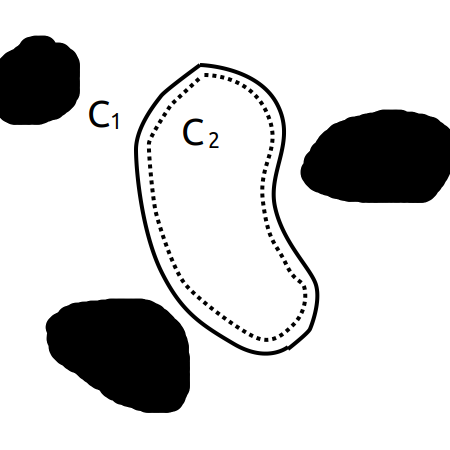
\includegraphics[width=4.cm, cframe=gray .2mm]{empty_closed.png}}
  \centerline{A}
\end{minipage}
\hfill
\begin{minipage}{.48\linewidth}
  \centerline{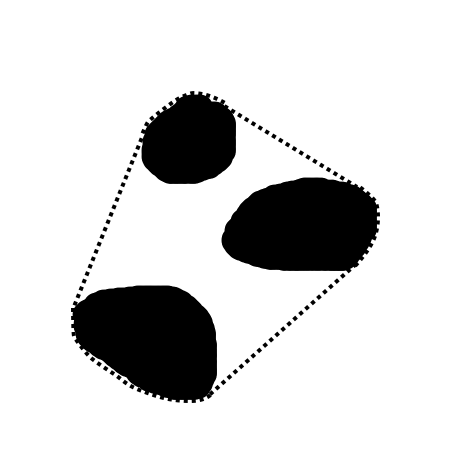
\includegraphics[width=4.cm, cframe=gray .2mm]{tangent_closed.png}}
  \centerline{B}
\end{minipage}
\vfill

\caption{Figure A shows an example of a closed curve ($C_1$, solid line) that encircles no obstacles and an inner curve ($C_2$, dotted line) in its neighboring region. Figure B shows a closed curve (dotted line) that consists of tangents, which encircles three obstacles. In this and all following figures, the white area represents passable grid states, and the black area represents impassable grid states.}
\label{closed_curve}
\end{figure}

\begin{myLemma}
For $\mathcal{S}_{2}$, there is no closed curve that encircles no obstacles, and any part of it is locally shortest.
\end{myLemma}                                                                                                                                                                                                                                                                                                                                                                                                                                                                                                                                                                                                                                                                                                                                                                                                                                                                                                                                                                                                                                                                                                                                                                                                                                                                                                                                                                                                                                                                                                                                                                                                                                                                                                                                                                                                                                                                                                                                                                                                                                                                                                                                                                                                                                                                                                                                                                                                                                                                                                                                                                                                                                                                                                                                                                                                                                                                                                                                                                                                                                                                                                                                                                                                                                                                                                                                                                                                                                                                                                                                                                    

\begin{myProof}
%In $\mathcal{C}_{2}$, for a closed curve $C_1$ that encircle no obstacle, we can always construct a shorter inner curve $C_2$ which is in the any small $\epsilon$-neighboring region of $C_1$. However, if any part of $C_1$ is locally shortest, $C_2$  should be longer than $C_1$, resulted in a contradiction. So, for a closed curve that encircle no obstacle, not every part of it is locally shortest, an example is shown in Fig. \ref{closed_curve}(A).
%On the contrast, for a closed curve that encircle obstacle, every part of it may be locally shortest. An example is a closed curve that consists of continuous tangents on the boundary of obstacle, which cannot find a shorter curve in its neighboring region, an example of such a closed curve is shown Fig. \ref{closed_curve}(B).

In $\mathcal{S}_{2}$, for a closed curve $C_1$ that encircles no obstacle, we can always construct a shorter inner curve $C_2$ which is in any small $\epsilon$-neighboring region of $C_1$. However, if any part of $C_1$ is locally shortest, $C_2$ should be longer than $C_1$, resulting in a contradiction. Therefore, for a closed curve that encircles no obstacle, not every part of it is locally shortest. An example is shown in Fig. \ref{closed_curve}(A).

In contrast, for a closed curve that encircles an obstacle, every part of it may be locally shortest. An example is a closed curve that consists of continuous tangents on the boundary of an obstacle, which cannot find a shorter curve in its neighboring region. An example of such a closed curve is shown in Fig. \ref{closed_curve}(B).

 
\end{myProof}

\begin{myTheo}
\label{core1}
For $\mathcal{S}_{2}$, any two locally shortest paths that share the same start and target cannot belong to the same homotopy class.
\end{myTheo}

\begin{figure}[t] \scriptsize
%\begin{tabular}{cc}
\begin{minipage}{.48\linewidth}
  \centerline{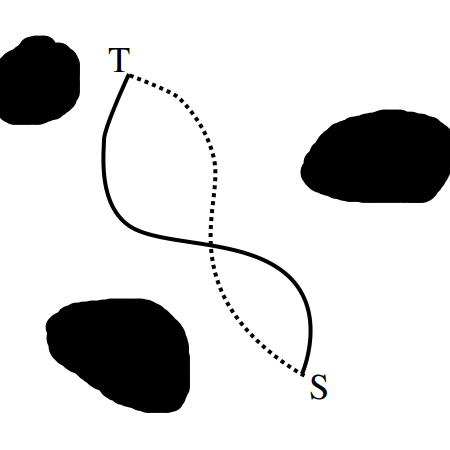
\includegraphics[width=4.cm, cframe=gray .2mm]{path_intersect.png}}
  \centerline{A}
\end{minipage}
\hfill
\begin{minipage}{.48\linewidth}
  \centerline{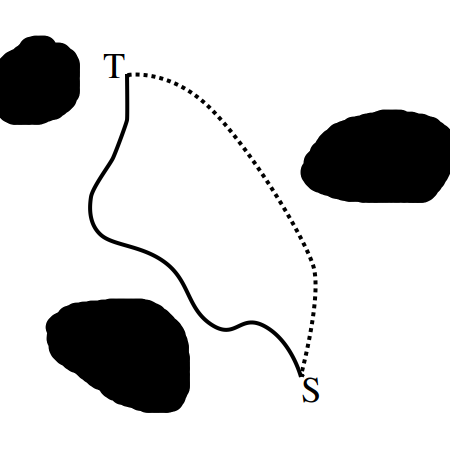
\includegraphics[width=4.cm, cframe=gray .2mm]{path_no_intersect.png}}
  \centerline{B}
\end{minipage}
\vfill

\caption{
For the two figures, solid lines and dotted lines represent different paths, "T" and "S" represent the common target and start of those paths, the same applies hereinafter. Figure A shows an example of two homotopic paths that intersect with each other, while Fig B shows an example of two paths that have no intersection with each other. As shown in Figure A and Figure B, two homotopic paths can always form at least one closed curve.
}
\label{path_intersect}
\end{figure}

\begin{myProof}
%Proof by contradiction. 
%For $\mathcal{C}_{2}$, assuming two locally shortest paths ($p_1$ and $p_2$) are in the same homotopy class, considering they share the same start and target, there exist at least one closed curve that encircle no obstacles formed by a part of $p_1$ and $p_2$, no matter whether $p_1$ and $p_2$ is intersecting with each other, related examples are shown in Fig. \ref{path_intersect}. However, this is contradict with that "for $\mathcal{C}_{2}$, there exist no a closed curve that encircle no obstacles and any part of it is locally shortest", so any two locally shortest paths that share the same start and target cannot belong to the same homotopy class.
For $\mathcal{S}_{2}$, assuming two locally shortest paths ($p_1$ and $p_2$) are in the same homotopy class, considering they share the same start and target, there exists at least one closed curve that encircles no obstacles formed by a part of $p_1$ and $p_2$, regardless of whether $p_1$ and $p_2$ intersect with each other. Related examples are shown in Fig. \ref{path_intersect}. However, this contradicts the statement that "for $\mathcal{C}_{2}$, there exists no closed curve that encircles no obstacles, and any part of it is locally shortest." Therefore, any two locally shortest paths that share the same start and target cannot belong to the same homotopy class.

\end{myProof}

\begin{myTheo}
\label{core3}
%For $\mathcal{C}_{3}$, two locally shortest paths that share the same start and target may belong to the same homotopy class. 
For $\mathcal{S}_{3}$, two locally shortest paths that share the same start and target may belong to the same homotopy class.

\end{myTheo}

\begin{figure}[t] \scriptsize
  \centerline{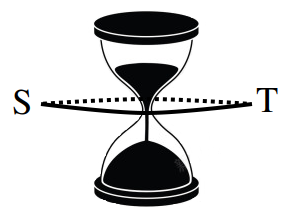
\includegraphics[width=3.cm]{example_3d.png}}
\caption{This figure shows an hourglass-shaped obstacle, and there are two locally shortest paths that share the same start and target ("S" and "T"). The straight line connecting the start and target is blocked by the narrow pipes in the center of the hourglass. One path bypasses the recess side of the "hourglass," while the other path bypasses the recess on the opposing side, and both of them are locally shortest. }
\label{example_3d}
\end{figure}

\begin{myProof}
% illustrate an example
Here we can illustrate an example for $\mathcal{S}_{3}$, as shown in Fig. \ref{example_3d}. Both of the two paths are locally shortest, and one can be transformed into another without intersecting with obstacles. So, for $\mathcal{S}_{3}$, two locally shortest paths that share the same start and target may belong to the same homotopy class.

\end{myProof}

Building upon this theoretical foundation, for $\mathcal{S}_{2}$, if $K$ locally shortest paths exist, we consequently obtain $K$ topologically distinctive paths. However, for $\mathcal{S}_{3}$, a locally shortest path may not correspond to a unique homotopy class.

\begin{myTheo}
For $\mathcal{S}_{2}$, locally shortest paths can be formed by tangents connecting the start and target points, as proven in \cite{8, 17}.
\end{myTheo}

In summary, for $\mathcal{S}_{2}$, utilizing the tangent graph allows the generation of multiple topologically distinctive paths, but this does not work for $\mathcal{S}_{3}$. Meanwhile, the time cost of tangent graph detection remains insensitive to the scale increase of maps, as the tangent graph is solely determined by the geometric elements of the maps. These advantages will be demonstrated and discussed in Section \ref{Results}.


\subsection{Algorithm}

In this section, we focus on the implementation of using the tangent graph to obtain multiple topologically distinctive paths. Building upon the theoretical foundation, we can extract multiple topologically distinctive paths from the tangent graph. Our focus in this section is on the efficient utilization of the tangent graph to obtain multiple topologically distinctive paths. Traditionally, two well-known methods for determining paths between two nodes in a graph are Breadth-First Search (BFS) and Best-First Search. Given that existing methods (refer to Section \ref{RelatedWork} for more details) often require multiple searches to obtain multiple paths, our objective is to find multiple paths in a single graph search. Consequently, we choose to implement our method based on Breadth-First Search.


\subsubsection{Construction of tangent graph}

Researchers have proposed several methods \cite{8, 17, 10} to generate tangent graphs from grid maps. Here, we choose ENL-SVG \cite{oh2017edge} to generate tangent graphs because it uses line-of-sight scans to construct the graph. Line-of-sight scans utilize a row-by-row scan to avoid point-to-point line-of-sight checks, which is very effective in maps with dense obstacles. However, for large grid maps with sparse obstacles, we replace the line-of-sight scan with Jump Over Block (JOB) \cite{10266687}, which accelerates LOS checks significantly under those maps.

Although the graph generated by ENL-SVG \cite{oh2017edge} was called a "visibility graph" in \cite{oh2017edge}, they use the taut condition to ensure local shortest paths, which is different from an ordinary visibility graph that only concerns visibility between nodes (i.e., waypoints). The taut condition imposes restrictions on any two connecting edges (i.e., three continuous waypoints) in the path. Informally, the taut condition is two connecting edges which, when treated as a string, cannot be made “tighter” by pulling on its ends. Some examples of the taut condition are shown in Fig. \ref{taut_condition}. A path is locally shortest only when any two continuous edges in it meet the taut condition.

The construction of the tangent graph is not the main purpose or contribution of this article. More details about the construction of the tangent graph can be found in \cite{oh2017edge}.


\begin{figure}[t]
\begin{minipage}{.32\linewidth}
  \centerline{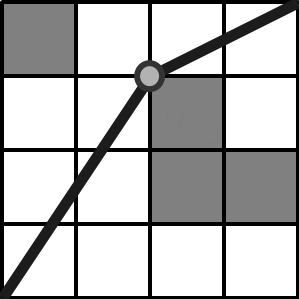
\includegraphics[width=2.4cm, cframe=gray .2mm]{taut_a.png}}
  \centerline{A}
\end{minipage}
\hfill
\begin{minipage}{.32\linewidth}
  \centerline{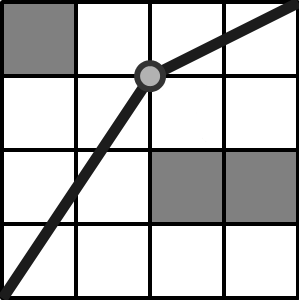
\includegraphics[width=2.4cm, cframe=gray .2mm]{taut_b.png}}
  \centerline{B}
\end{minipage}
\hfill
\begin{minipage}{.32\linewidth}
  \centerline{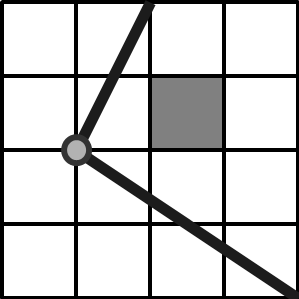
\includegraphics[width=2.4cm, cframe=gray .2mm]{taut_c.png}}
  \centerline{B}
\end{minipage}
\vfill
\caption{These figures show three examples of the taut condition, where (A) is taut, while (B) and (C) are not. These figures are quoted from \cite{oh2017edge}.
}
\label{taut_condition}
\end{figure}
   
\subsubsection{Loop avoidance}

\begin{figure}[t]
\begin{minipage}{.48\linewidth}
  \centerline{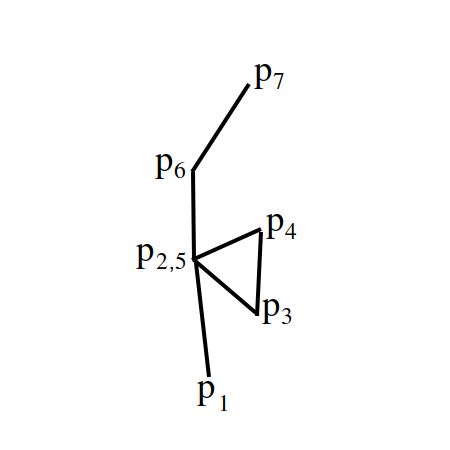
\includegraphics[width=2.7cm, cframe=gray .2mm]{overlap_wp.png}}
  \centerline{A}
\end{minipage}
\hfill
\begin{minipage}{.48\linewidth}
  \centerline{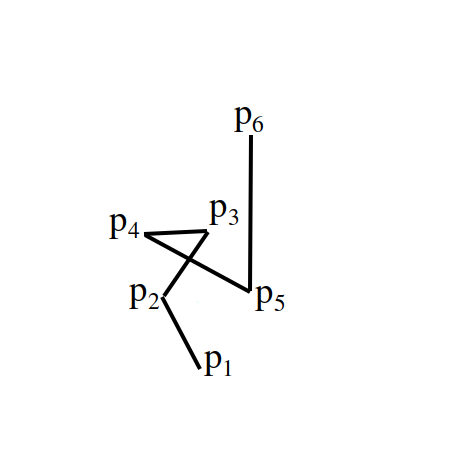
\includegraphics[width=2.7cm, cframe=gray .2mm]{line_intersect.png}}
  \centerline{B}
\end{minipage}
\vfill
\caption{These figures show examples of two possible states of loops in a path. Figure A shows loops caused by the revisitation of waypoints ($p_2$ and $p_5$), while Figure B shows loops caused by line intersection ($p_2\rightarrow p_3$ and $p_4\rightarrow p_5$). The order of waypoints is shown in increasing numbers. For example, in Figure A, $p_{1}$ is the first waypoint, and $p_{2,5}$ means the second and the fifth waypoints are overlapped. }
\label{two_loops}
\end{figure}

As a fundamental principle in topologically distinctive paths \cite{bhattacharya2012topological}, path planning with distinctive topology strictly avoids the presence of loops. Loops in this context can take two forms: 1) overlap waypoint, where a waypoint is revisited within a single path; 2) line intersection, where two lines of the path intersect with each other, as shown in Fig. \ref{two_loops}.

So, there are two steps to check whether a path has loops when adding a new waypoint: the first step is to check whether the new node has already occurred in the path; the second step is to check whether the newly added edge (the connection of the new node and the last node of the path) intersects with other edges in the path. If there is no such revisitation or intersection, the addition of the new node passes the loop avoidance check.

Notably, as the number of waypoints in a path increases, the time required for loop detection also grows. In detail, when checking whether adding a waypoint to a path with $n$ waypoints, $n$ revisitation checks and $n-1$ line intersection checks are performed. If a finished path has $n$ waypoints, it takes $\frac{(n-1)n}{2}$ revisitation checks and $\frac{(n-2)(n-1)}{2}$ line intersection checks in total before it reaches the target. We analyzed the time cost component of path search via Perf\footnote{https://www.jetbrains.com/help/clion/cpu-profiler.html} and found that loop avoidance takes 50\% to 80\% of the total time cost on average.



\subsubsection{Path search} 

\begin{figure*}[t]
\begin{minipage}{.23\linewidth}
  \centerline{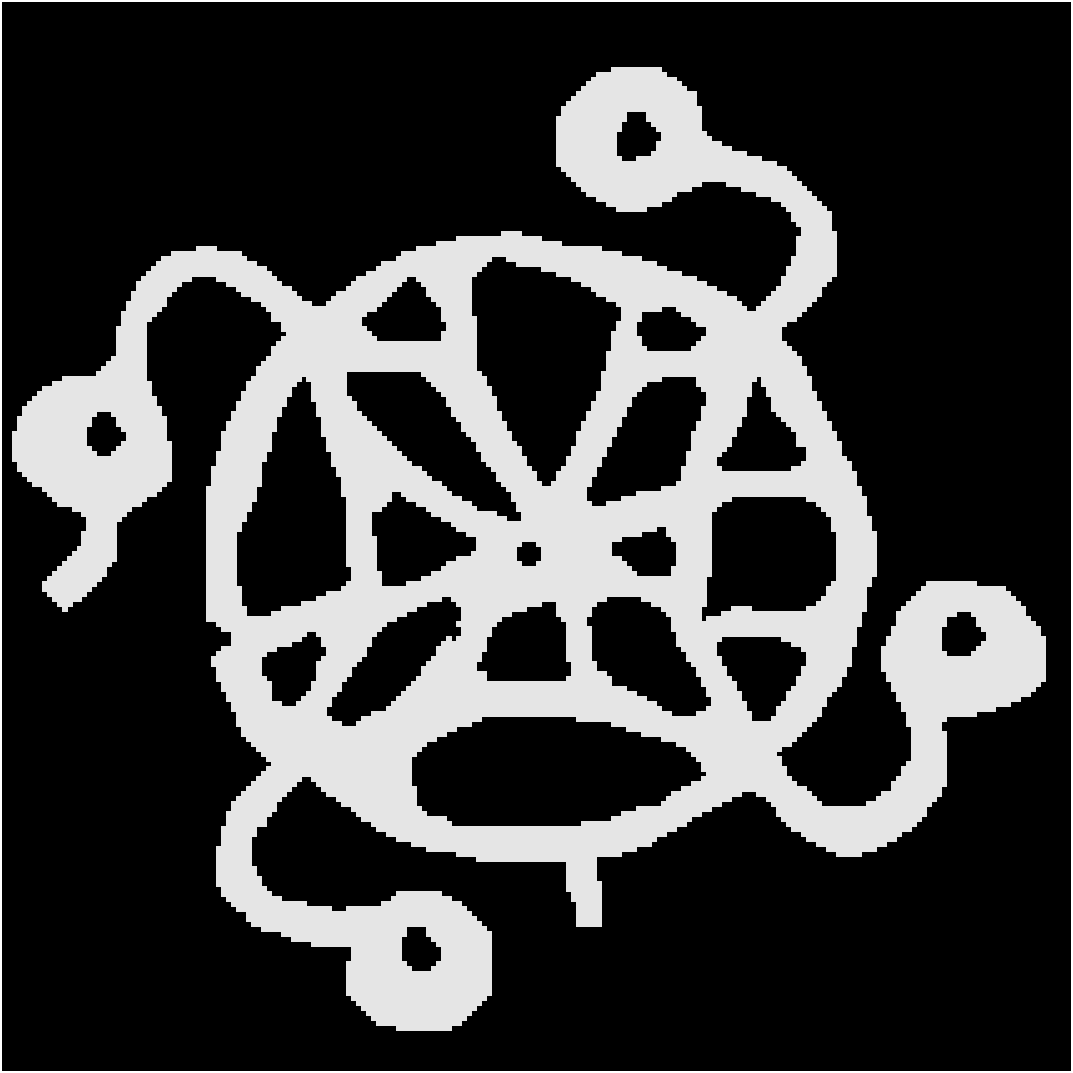
\includegraphics[width=4.2cm, cframe=gray .2mm]{map.png}}
  \centerline{A}
\end{minipage}
\hfill
\begin{minipage}{.23\linewidth}
  \centerline{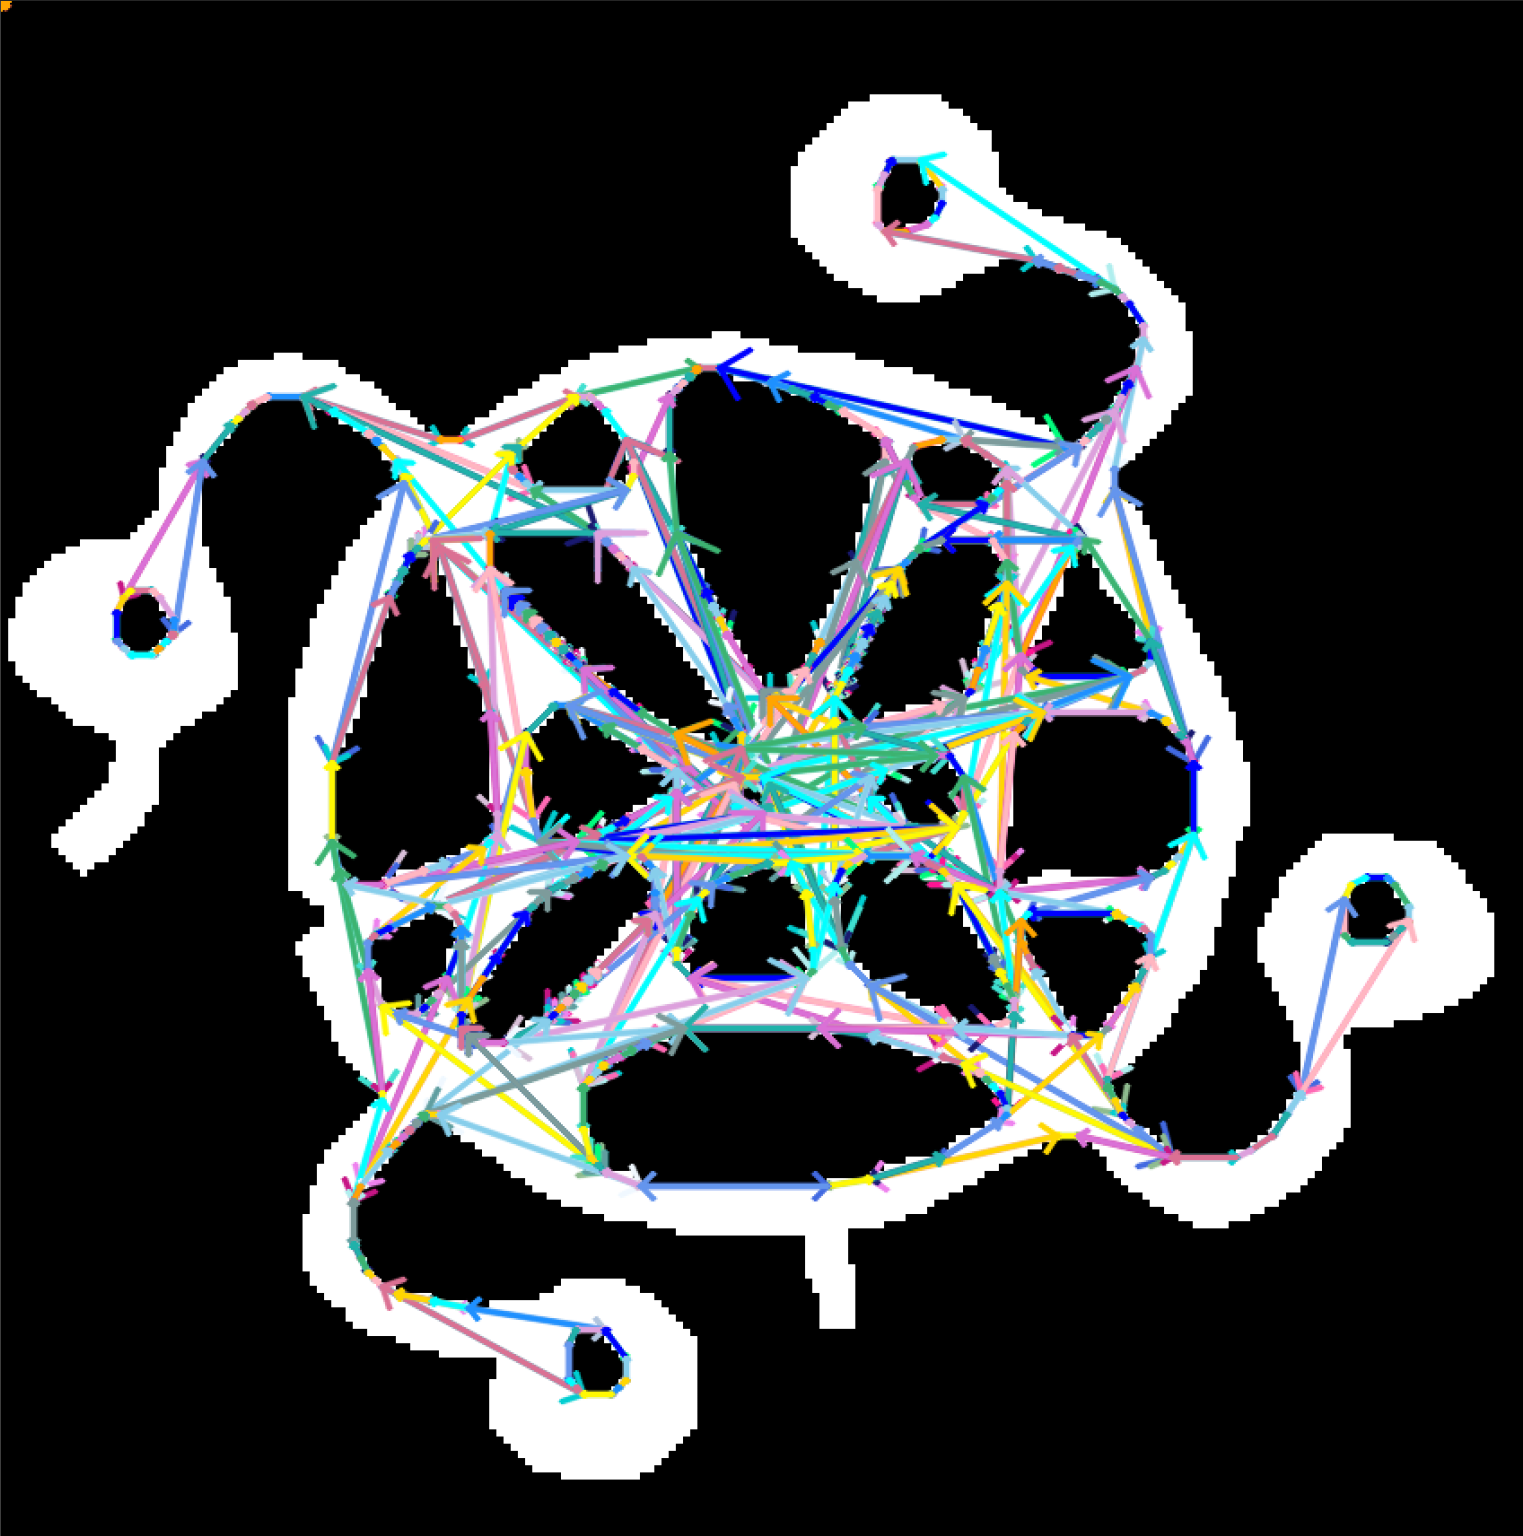
\includegraphics[width=4.2cm, cframe=gray .2mm]{map1.png}}
  \centerline{B}
\end{minipage}
\hfill
\begin{minipage}{.23\linewidth}
  \centerline{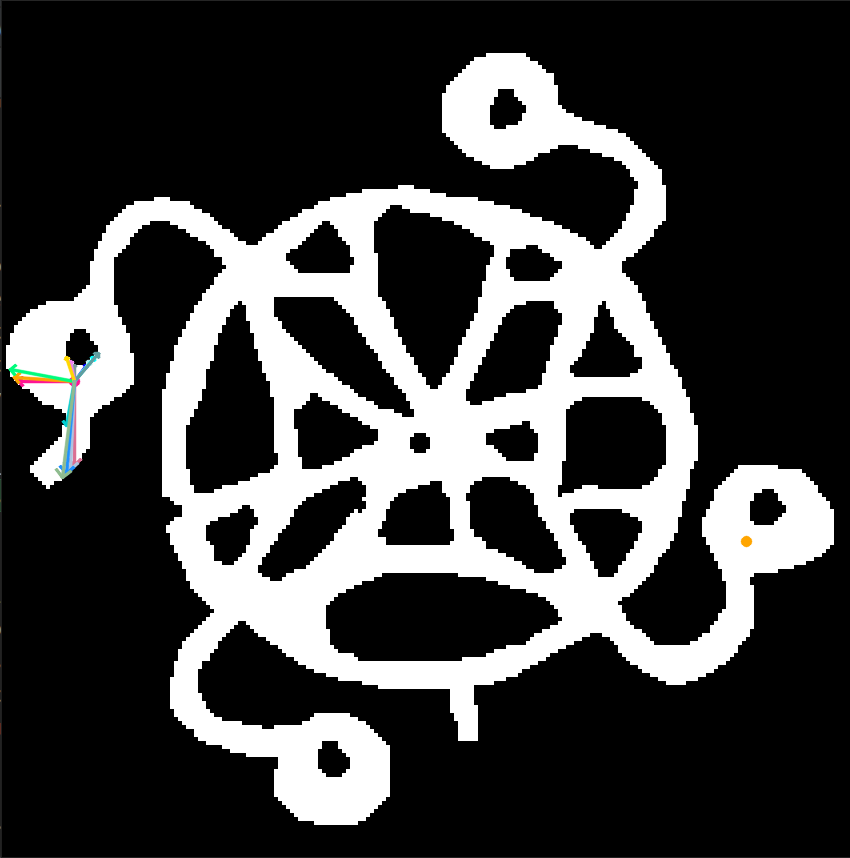
\includegraphics[width=4.2cm, cframe=gray .2mm]{map2.png}}
  \centerline{C}
\end{minipage}
\hfill
\begin{minipage}{.23\linewidth}
  \centerline{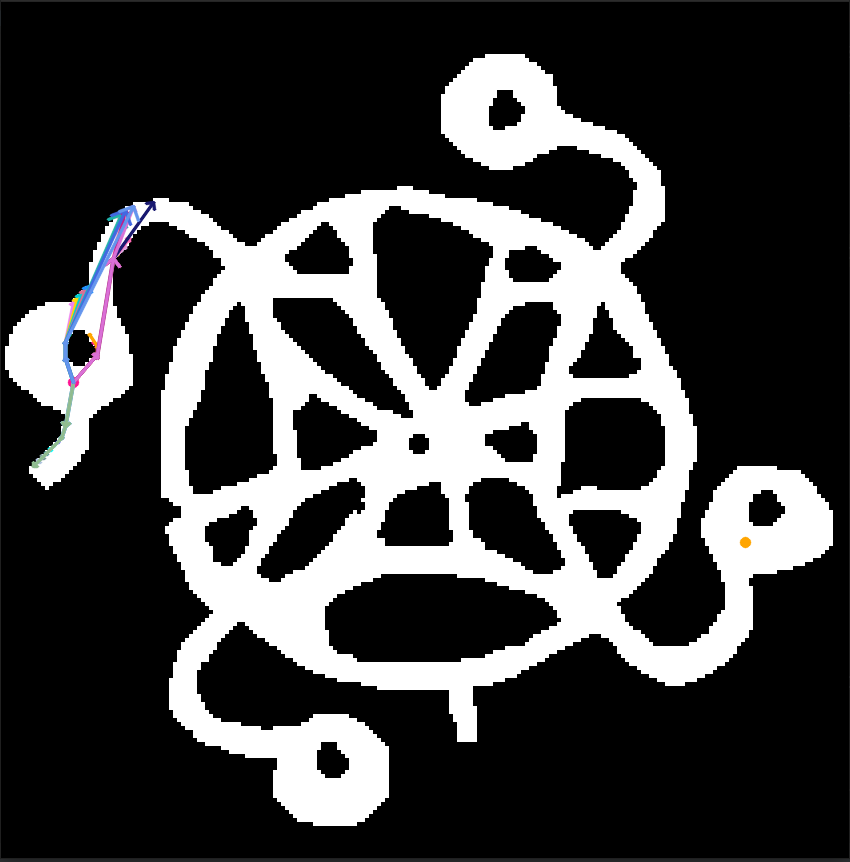
\includegraphics[width=4.2cm, cframe=gray .2mm]{map3.png}}
  \centerline{D}
\end{minipage}
\vfill
\begin{minipage}{.23\linewidth}
  \centerline{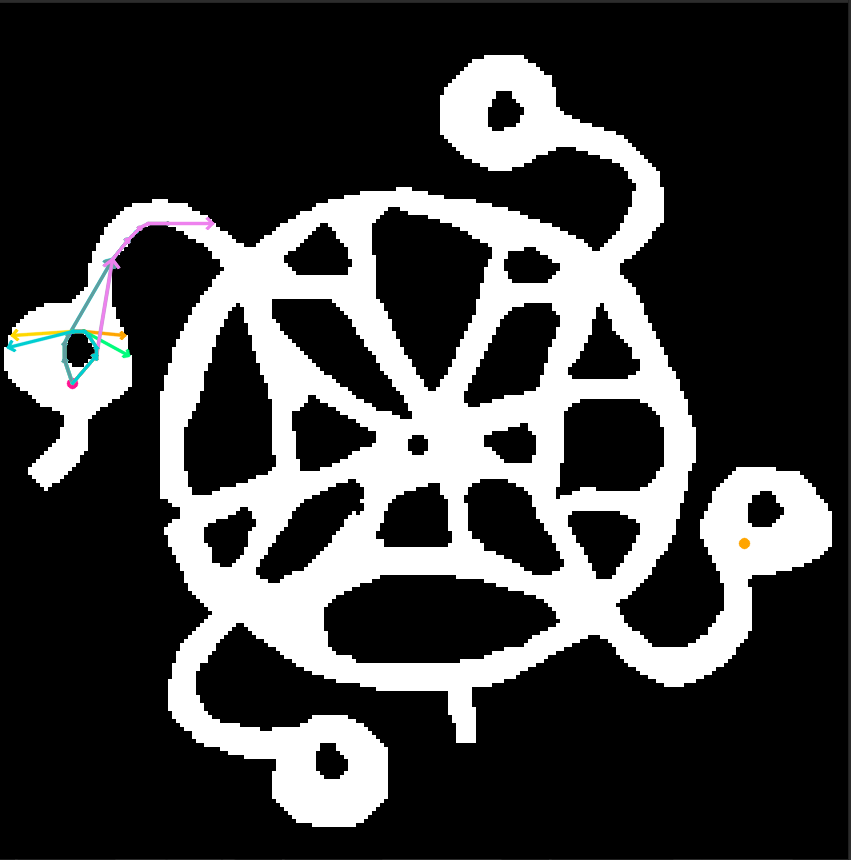
\includegraphics[width=4.2cm, cframe=gray .2mm]{map4.png}}
  \centerline{E}
\end{minipage}
\hfill
\begin{minipage}{.23\linewidth}
  \centerline{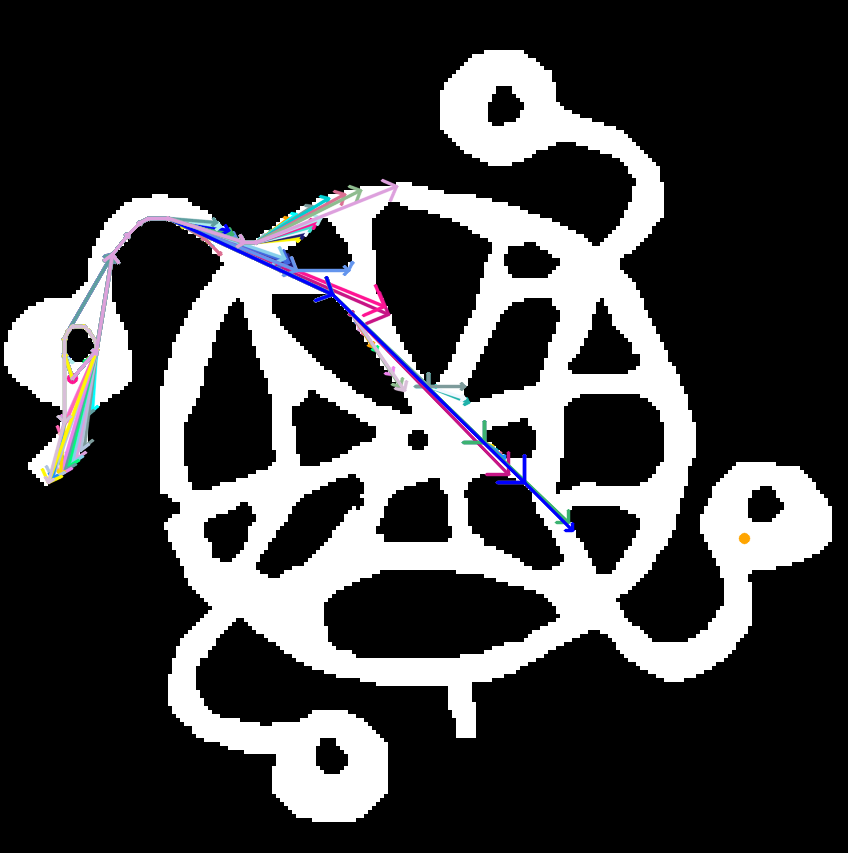
\includegraphics[width=4.2cm, cframe=gray .2mm]{map5.png}}
  \centerline{F}
\end{minipage}
\hfill
\begin{minipage}{.23\linewidth}
  \centerline{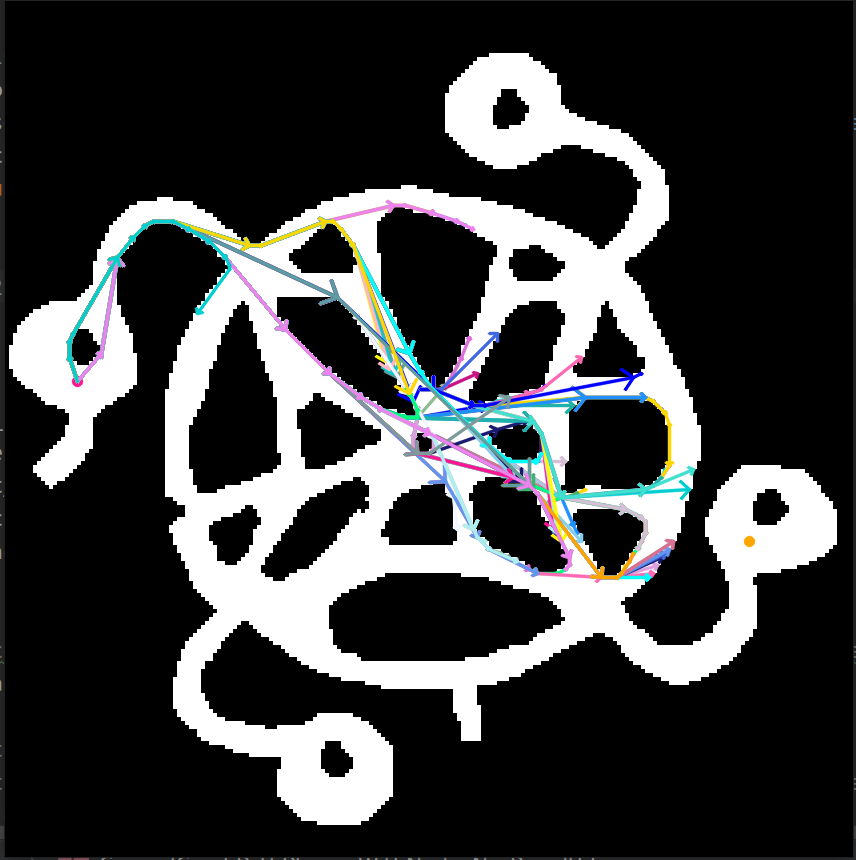
\includegraphics[width=4.2cm, cframe=gray .2mm]{map6.png}}
  \centerline{G}
\end{minipage}
\hfill
\begin{minipage}{.23\linewidth}
  \centerline{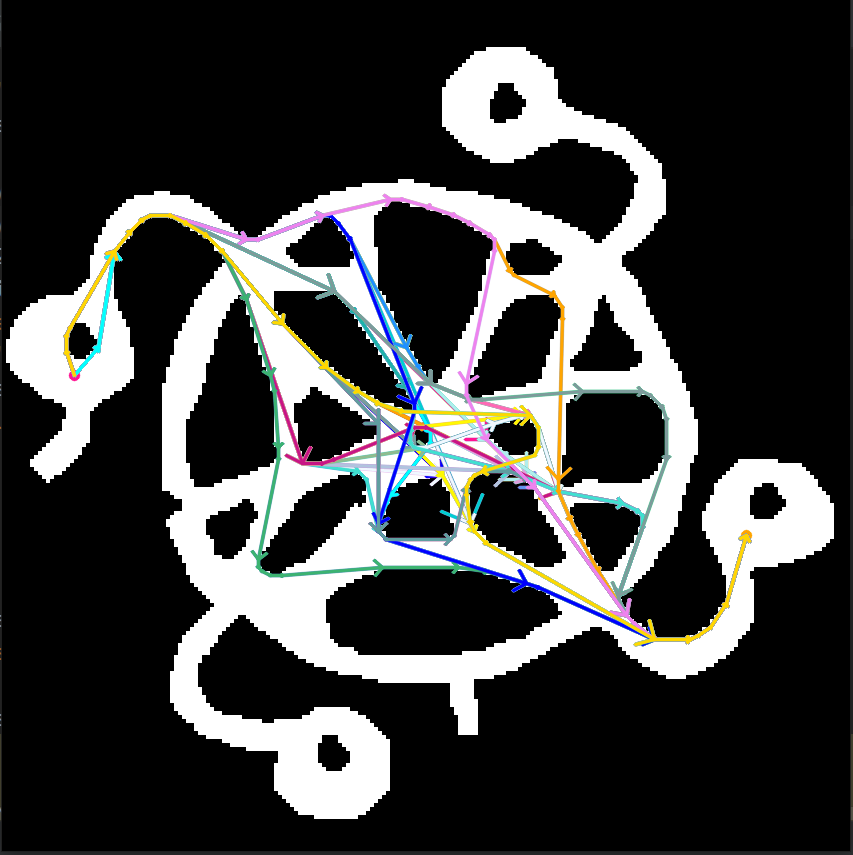
\includegraphics[width=4.2cm, cframe=gray .2mm]{map7.png}}
  \centerline{H}
\end{minipage}
\vfill
\caption{
These figures show the whole process of our algorithm. Figure A shows the raw grid map; Figure B shows the tangent graph of the grid map, with colored arrows representing all edges and their orientation. For a better visual effect, only edges that form loops are shown in different colors; Figure C shows the newly added edges connecting the start (point in the left-center of the map); Figures D to H show the Breadth-First search that starts from the newly added edges and ends when 100 paths are found. The map is AR0205SR with a size of 212*214, introduced from \cite{sturtevant2012benchmarks}. The start and target are (18, 95) and (186, 135) respectively, with the origin of the map being the upper-left corner.
}
\label{path_search}
\end{figure*}

\begin{algorithm}[t] 
 \normalem
\label{a1}
  \caption{Topology-aware Breadth First Search}
  \KwIn{$g_s, g_t, G(V, E), K$}  
  \KwOut{$P$}
  $P = \{g_s\}, P' = \emptyset, P_f = \emptyset$; \\
  add $g_s$ and $g_t$ to $G$; \\
  \While{find no $K$ paths and $P$ is not empty} {
  	 $P' = \emptyset$; \\
     \For{each unfinished path $p$ in $P$} {
     	\For{each nodes $v$ of $G$ that connect to last nodes of $p$}{
     	$p'$ = add $v$ to $p$; \\
     	\If{$p'$ have no loops and $p'$ meet taut condition}{
     	\eIf{$p'$ reach $g_t$} {
     	add $p'$ to $P'$; \\
     	}{
     	add $p'$ to $P_f$; \\
     	}
     	}
     	}	
     }
     $P = P'$ ; \\		  
  } 
  return $P_f$;
\end{algorithm}

\begin{table}[t]
	\centering  % 显示位置为中间
	\caption{Table of notations}  % 表格标题
	\label{table_of_notation}  % 用于索引表格的标签
	%字母的个数对应列数,|代表分割线
	% l代表左对齐,c代表居中,r代表右对齐
	\begin{tabular}{|c|c|c|c|}  
		\hline 
		%& & & \\[-6pt]  %可以避免文字偏上来调整文字与上边界的距离
		Name & Meanning & Name & Meanning \\  
		\hline
		$g_s$   & start point & $g_t$ & target point \\
		\hline
		$P, P'$ & set of unfinished path & $P_f$ & set of finished path \\
		\hline		
		$G(V, E)$ & tangent graph & $v$ & a node in tangent graph \\
		\hline		
		$p, p'$ & path & $P_B$ & \makecell[c]{set of unifinished path \\ (backup queue)} \\
		\hline
		%\hline
	\end{tabular}
\end{table}


Our method comprises two key components: tangent graph construction and path search. Tangent graph detection from grid maps is a well-explored area, and there exist established methods for this purpose \cite{8, 17, 10}. Considering the efficiency of line-of-sight scans, we adopt ENL-SVG\cite{oh2017edge} to construct our tangent graph. Consequently, our primary focus in this manuscript lies in the efficient search for paths.

We have modified the classical Breadth-First Search (BFS) algorithm used in graph search-based path planning to search for multiple topologically distinctive paths. In detail, there are three major modifications:

1. Using a tangent graph rather than other kinds of graphs;
 
2. Exiting when finding the required number of paths (i.e., K paths) rather than exiting when finding the first finished path;

3. Adding the taut condition\cite{oh2017edge} and loop avoidance as constraints during expansion to ensure locally shortest paths and reduce the search space, as outlined in Algorithm \ref{a1}. It is noteworthy that if there is no K path, the set $P$ will be empty after find all possible solutions, then the main loop will exit when the set $P$ is empty.

The notation used in the pseudocode is detailed in Table \ref{table_of_notation}, assuming the required number of paths is denoted as $K$. An illustrative example of path search is provided in Fig. \ref{path_search}. 

For some scenarios that require considering the volume of the moving agent, three steps are required:
1, inflate all obstacles of the grid map with the length of the maximum inscribed circle radius of the shape of the moving object;
2, run the topology-aware path search;
3, check whether each path is safe with consideration of the volume of the moving object and only keep all safe paths.


\begin{algorithm}[t] 
 \normalem
\label{a2}
  \caption{Topology-aware Breadth First Search with expansion reduction}
  \KwIn{$g_s, g_t, G(V, E), K$}  
  \KwOut{$P$}
  $P = \{g_s\}, P' = \emptyset, P_f = \emptyset, $\hl{$P_B = \emptyset$}; \\
  add $g_s$ and $g_t$ to $G$; \\
  \While{$P_f$ have no $K$ paths and $P$ is not empty} {
     $P' = \emptyset$; \\
     \For{each unfinished path $p$ in $P$} {
     	\For{each nodes $v$ of $G$ that connect to last nodes of $p$}{
     	$p'$ = add $v$ to $p$; \\
     	\If{$p'$ have no loops and $p'$ meet taut condition}{
     	\eIf{$p'$ reach $g_t$} {
     	add $p'$ to $P'$; \\
     	} {
     	add $p'$ to $P_f$; \\
     	}
     	}
     	}	
     }
     \hl{$P = \emptyset$;} \\
     \hl{sort $P'$ in increasing heurstic value;} \\
     \hl{move first $K$ path of $P'$ to $P$ and move remaining path in $P'$ to $P_B$;} \\
     \hl{sort $P_B$ in increasing heurstic value;} \\
     \If{\hl{$P$ have no $K$ paths}} {
	  \While{\hl{$P_B$ is not empty and $P$ have no $K$ path}} {
	  \hl{move path with minimum heurstic value in $P_B$ to $P$;} \\	  
	  }     
     }		  		  
  } 
  return $P_f$;
\end{algorithm}


\subsubsection{Expansion reduction}  

\begin{figure}[t] \scriptsize
%\begin{tabular}{cc}
\begin{minipage}{.48\linewidth}
  \centerline{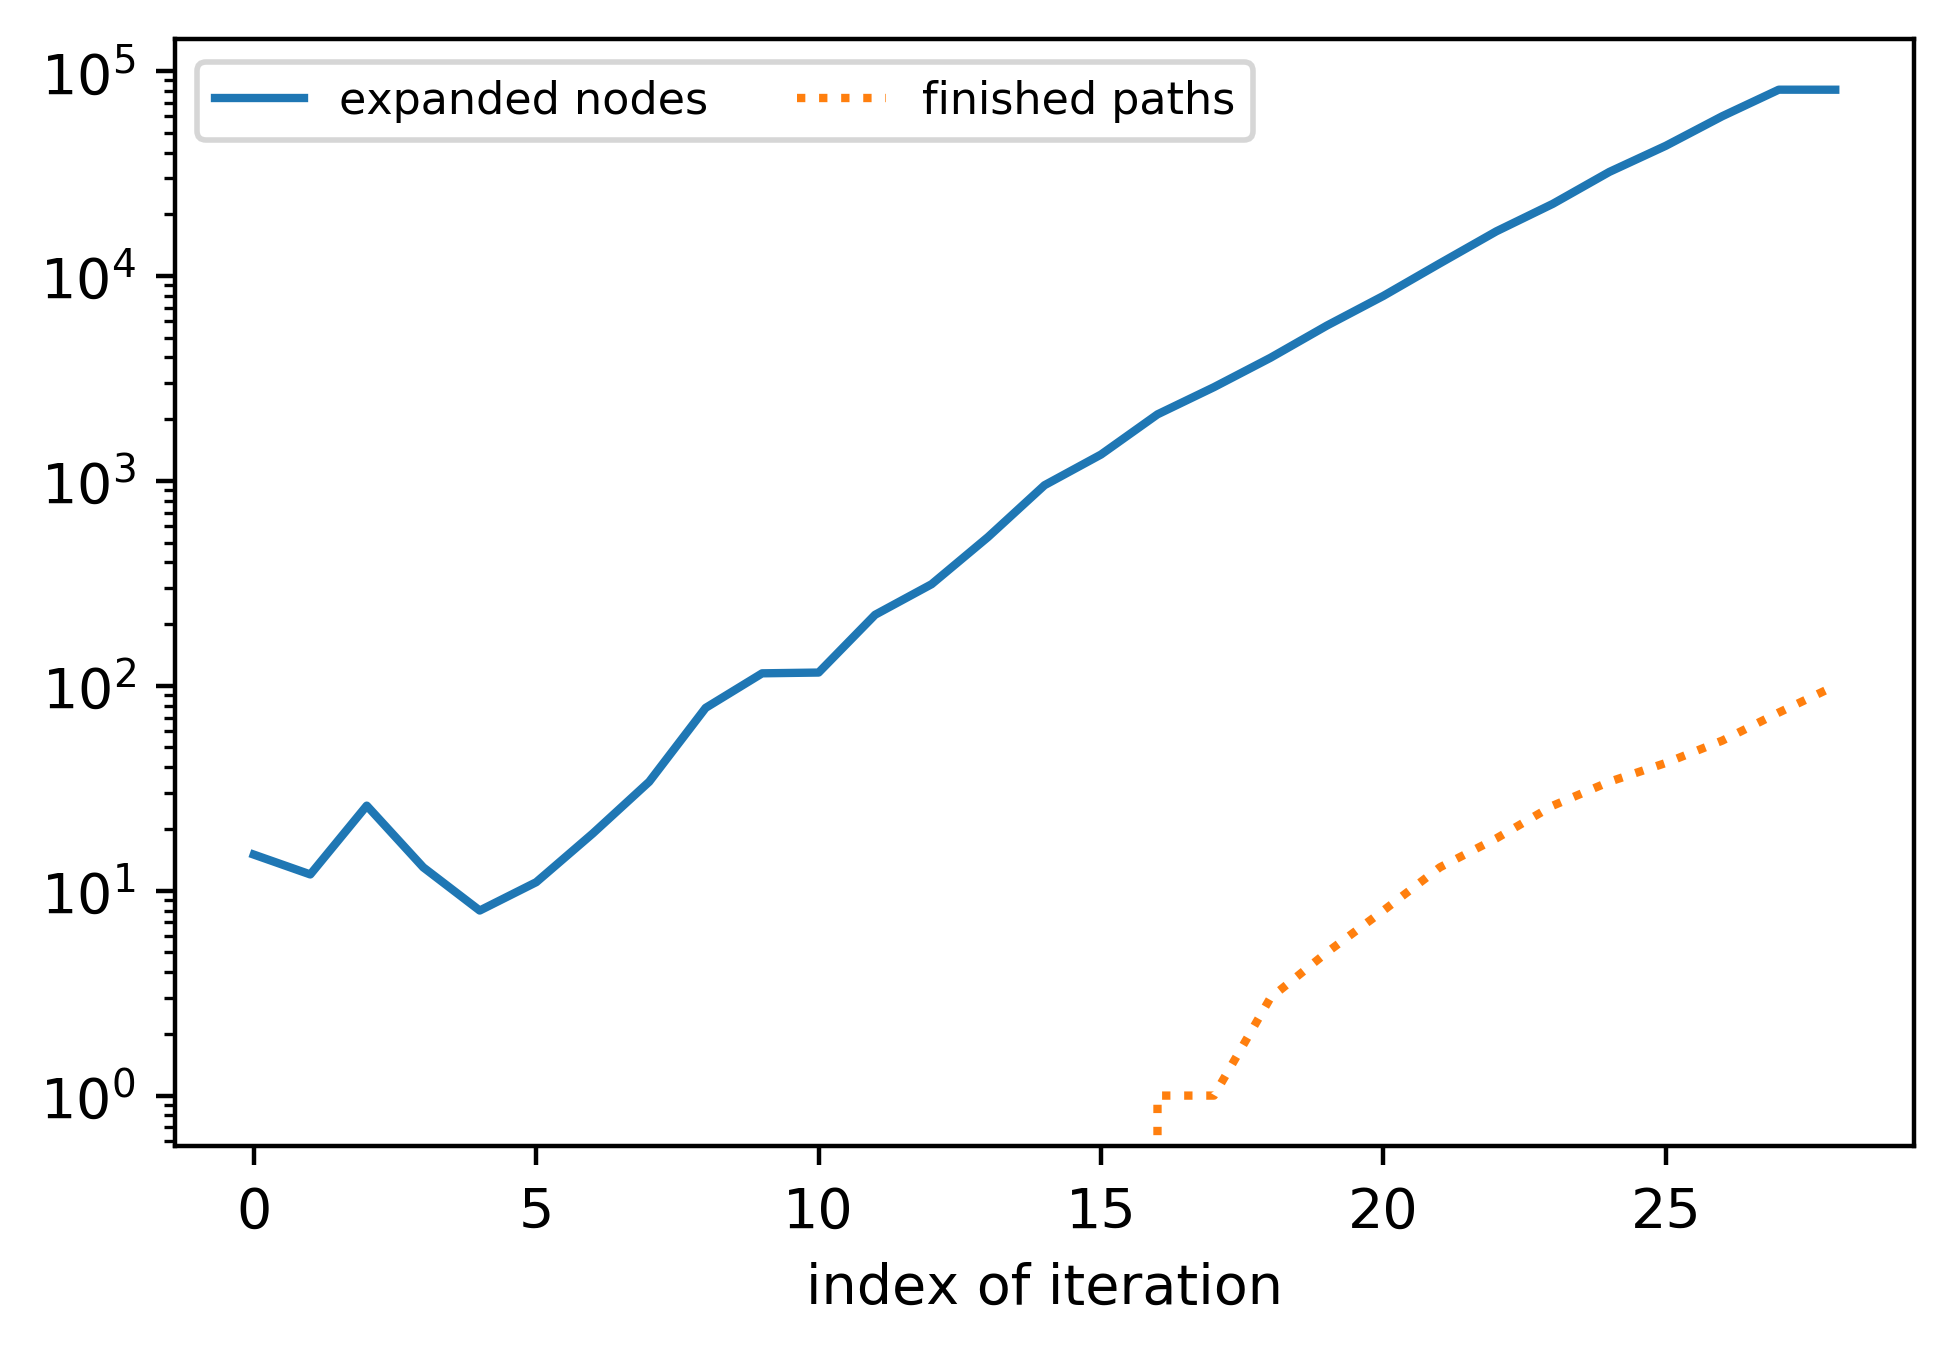
\includegraphics[width=4.6cm]{no_expansion.png}}
  \centerline{A: no expansion reduction}
\end{minipage}
\hfill
\begin{minipage}{.48\linewidth}
  \centerline{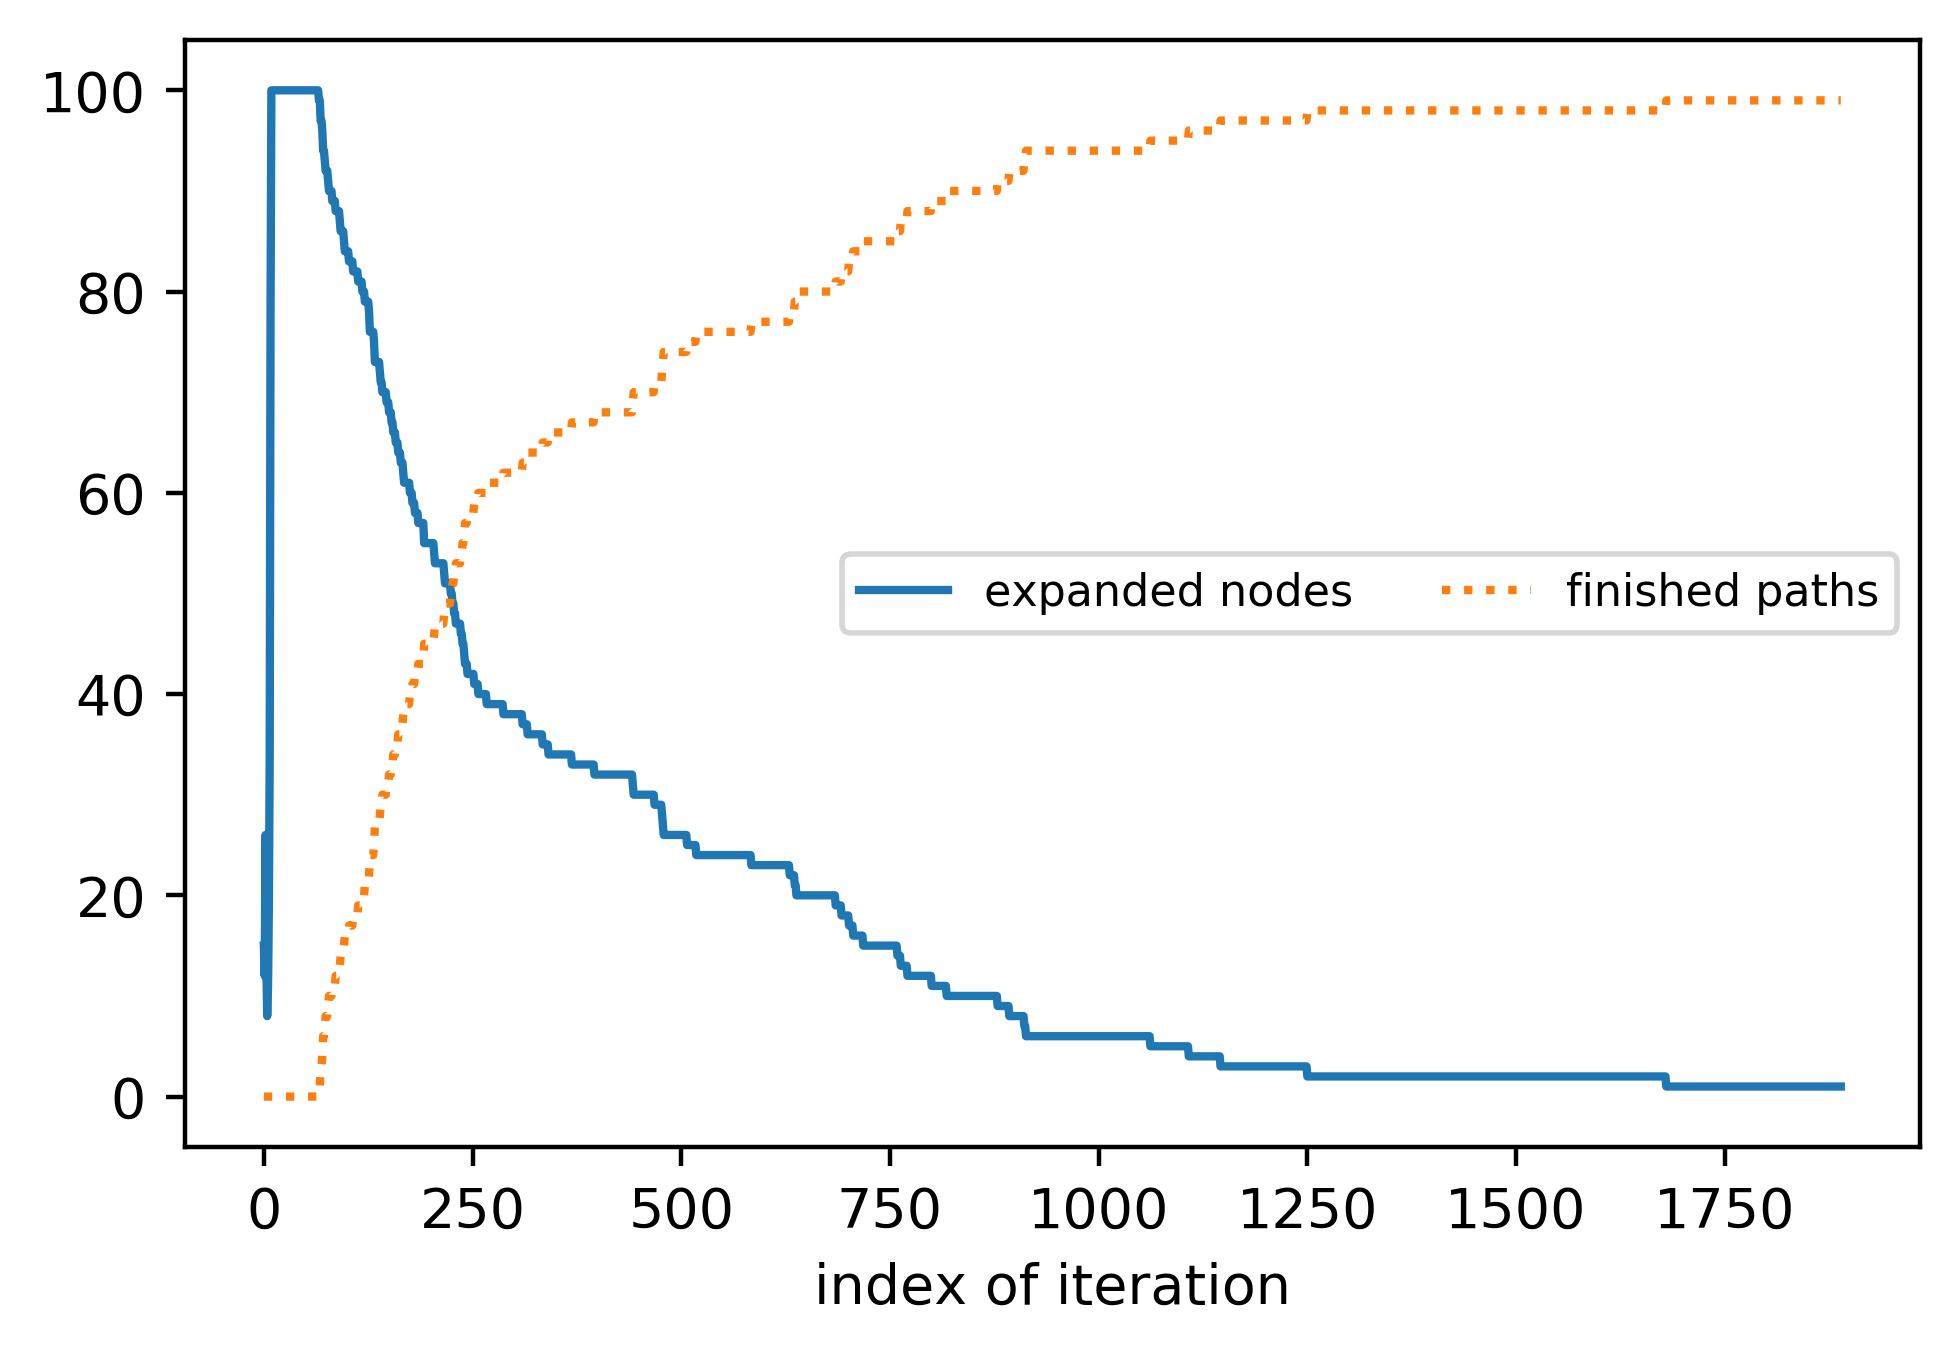
\includegraphics[width=4.6cm]{with_expansion.png}}
  \centerline{B: using expansion reduction}
\end{minipage}
\vfill

\caption{These two figures present the number of nodes expanded and the number of paths finished (i.e., reaching the target) during each iteration of path search when no expansion reduction is applied (Algorithm \ref{a1}, Figure A) and when using expansion reduction (Algorithm \ref{a2}, Figure B). It is noteworthy that Figure A uses a logarithmic coordinate system while Figure B does not.
}
\label{expansion_reduction_comparison}
\end{figure}
  
%One drawback of Algorithm \ref{a1} is the exponential growth in the size of unfinished paths as the number of expansions increases. To address this issue, we propose an expansion reduction technique to mitigate the exponential growth during iterations of BFS. This technique involves splitting the queue into two: a priority queue and a backup queue.

%In each iteration of BFS, we select the top $K$ paths with the minimal heuristic value (calculated in the same manner as A*) and store them in the priority queue as candidates for expansion. The remaining unfinished paths are cached in a backup queue, sorted by their heuristic values.

%If there are fewer than $K$ unfinished paths in the priority queue, we extract unfinished paths from the backup queue and insert them into the priority queue until there are $K$ elements in the priority queue or the backup queue is empty, as shown in Algorithm \ref{a2}. The relevant code related to the priority queue has been highlighted.

One drawback of Algorithm \ref{a1} is the exponential growth in the size of unfinished paths as the number of expansions increases. To address this issue, we propose an expansion reduction technique to mitigate the exponential growth during iterations of BFS. This technique involves splitting the queue into two: a priority queue and a backup queue.

In each iteration of BFS, we select the first $K$ paths with the minimal heuristic value (calculated in the same manner as A*) and store them in the priority queue as candidates for expansion. The remaining unfinished paths are cached in a backup queue, sorted by their heuristic values.

If there are fewer than $K$ unfinished paths in the priority queue, we extract unfinished paths from the backup queue and insert them into the priority queue until there are $K$ elements in the priority queue or the backup queue is empty, as shown in Algorithm \ref{a2}. The relevant code related to the expansion reduction has been highlighted.


%Essentially, this approach changes the order of expansion of unfinished paths, prioritizing paths that are closer to the target (i.e., have lower heuristic values). As a result, the path search concludes sooner compared to the scenario without expansion reduction. Importantly, the expansion reduction does not compromise completeness. Algorithm \ref{a2} outlines BFS with expansion reduction, specifying its differences compared to Algorithm \ref{a1}.

%An illustrative example highlighting the benefits of introducing expansion limitation is presented in Fig. \ref{expansion_reduction_comparison}. 
%All configuration about path search are the same as the case in Fig. \ref{path_search}. The only different is whether introduce expansion reduction. 

%When no expansion reduction, the total time cost of path search is 573.9 ms and the number of nodes expanded during each iteration is growing in an exponential manner, stop when required number ($K=100$) of path reach target. 374662 node expansion are perfomed during path search and most of them are irrelevant with finished paths.

%But when using expansion reduction, the total time cost of path search is 133.2 ms and the number of nodes expanded stop growing when it reach 100, then decreases as more and more paths reach target. Thus only 36385 expansion are performed and most of them are relevant with finished path. 

%Although using expansion reduction taking more iteration than no expansion reduction, but there is only a few nodes are expanded during each iteration, as shown in Fig. \ref{expansion_reduction_comparison}. In summary, the introduction of expansion reduction reduce the time cost of path search significantly by reduce the times of node expansion.  

Essentially, this approach changes the order of expansion of unfinished paths, prioritizing paths that are closer to the target (i.e., have lower heuristic values). As a result, the path search concludes sooner compared to the scenario without expansion reduction. Importantly, the expansion reduction does not compromise completeness or path's locally shortest property. Algorithm \ref{a2} outlines BFS with expansion reduction, specifying its differences compared to Algorithm \ref{a1}.

An illustrative example highlighting the benefits of introducing expansion reduction is presented in Fig. \ref{expansion_reduction_comparison}. All configurations for path search are the same as the case in Fig. \ref{path_search}. The only difference is whether to introduce expansion reduction.

When no expansion reduction is applied, the total time cost of path search is 573.9 ms, and the number of nodes expanded during each iteration grows exponentially, stopping when the required number ($K=100$) of paths reach the target. A total of 374662 node expansions are performed during path search, and most of them are irrelevant to finished paths.

However, when using expansion reduction, the total time cost of path search is only 133.2 ms, and the number of nodes expanded stops growing when it reaches 100, then decreases as more and more paths reach the target. Thus, only 36385 expansions are performed, and most of them are relevant to finished paths.

Although using expansion reduction takes more iterations than no expansion reduction, there are only a few nodes expanded during each iteration, as shown in Fig. \ref{expansion_reduction_comparison}. In summary, the introduction of expansion reduction significantly reduces the time cost of path search by reducing the number of node expansions.


%\begin{figure*}[t]
%\centering
%\vspace*{8pt}
%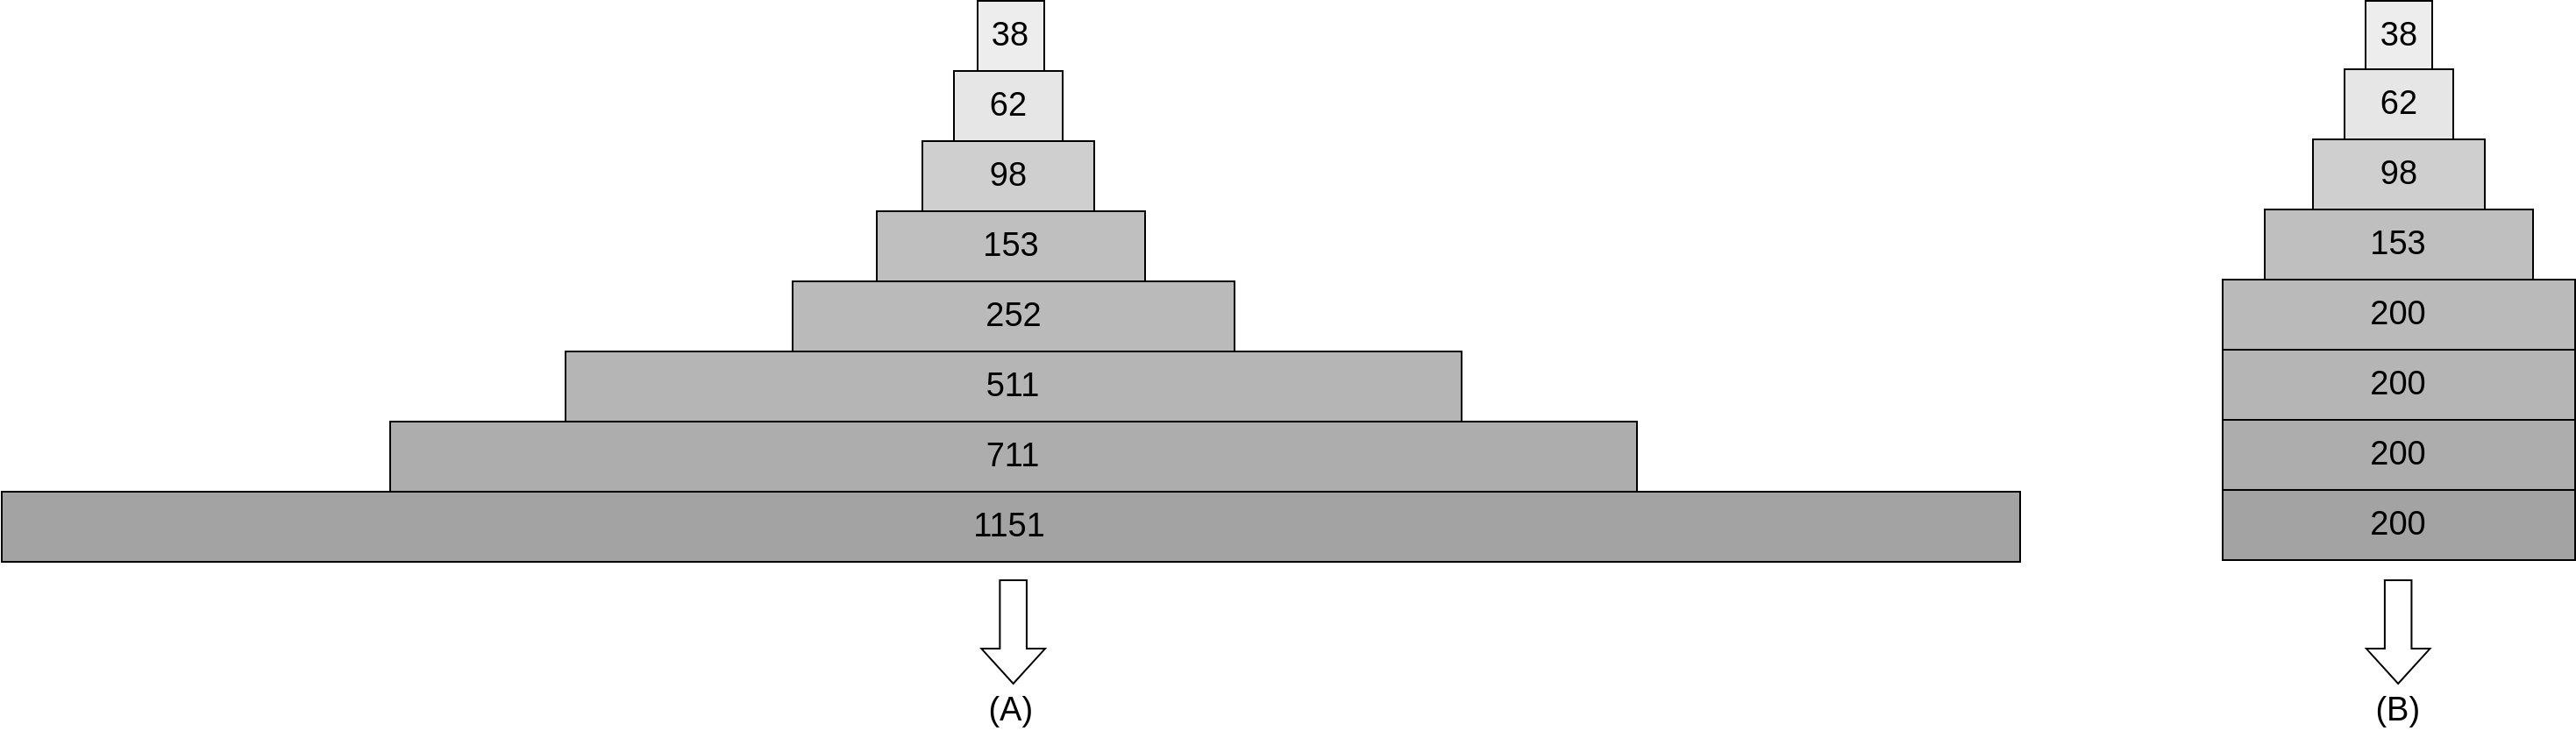
\includegraphics[width=12.5cm]{priority.png}
%\caption{These figures depict the changes in queue size during BFS expansion before (Figure A) and after (Figure B) implementing expansion reduction in the same scenario (Fig. \ref{examples}), where the goal is to find 200 paths. In both Figures A and B, it's evident that the queue size grows exponentially before the introduction of expansion reduction, but stabilizes once it reaches 200 after implementing this enhancement. Consequently, obtaining 200 paths takes 48.5ms before the introduction of expansion reduction, while it only takes 16.8ms afterward.
%} 
%\label{priority}
%\end{figure*}



\begin{figure}[t] \scriptsize
%\begin{tabular}{cc}
\begin{minipage}{.24\linewidth}
  \centerline{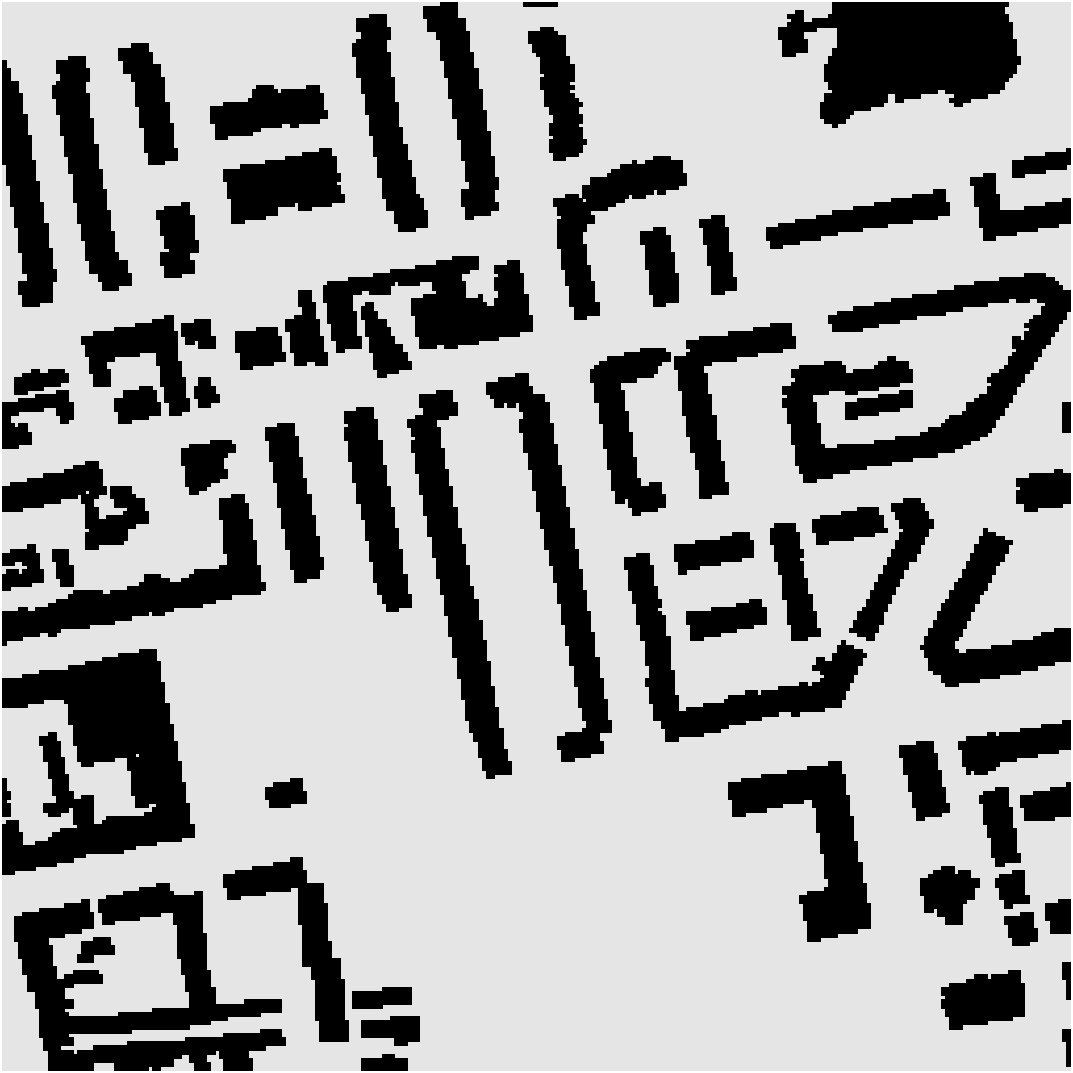
\includegraphics[width=2.1cm]{Berlin_1_256.png}}
  \centerline{A: Berlin\_1\_256}
\end{minipage}
\hfill
\begin{minipage}{.24\linewidth}
  \centerline{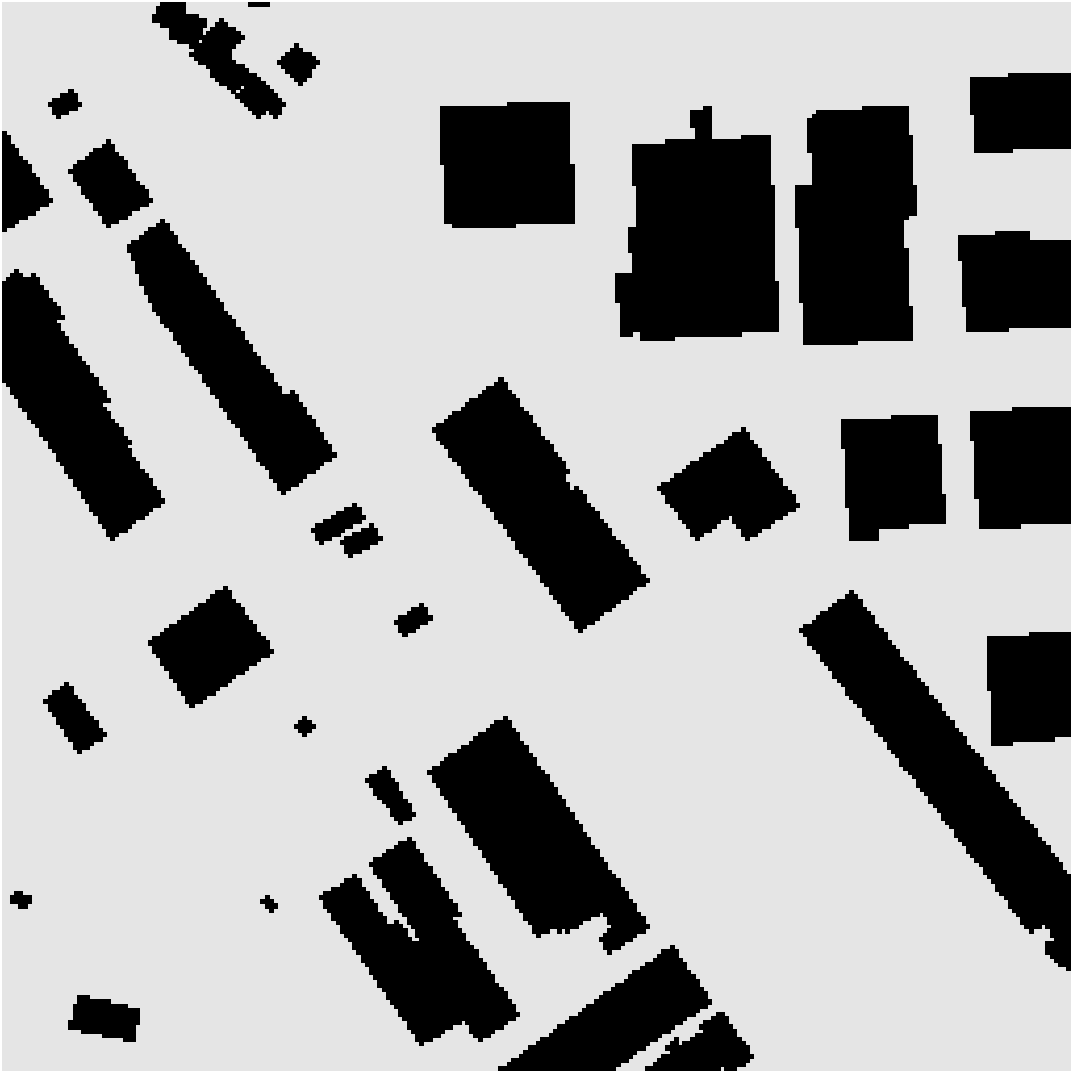
\includegraphics[width=2.1cm]{Boston_2_256.png}}
  \centerline{B: Boston\_2\_256}
\end{minipage}
\hfill
\begin{minipage}{.24\linewidth}
  \centerline{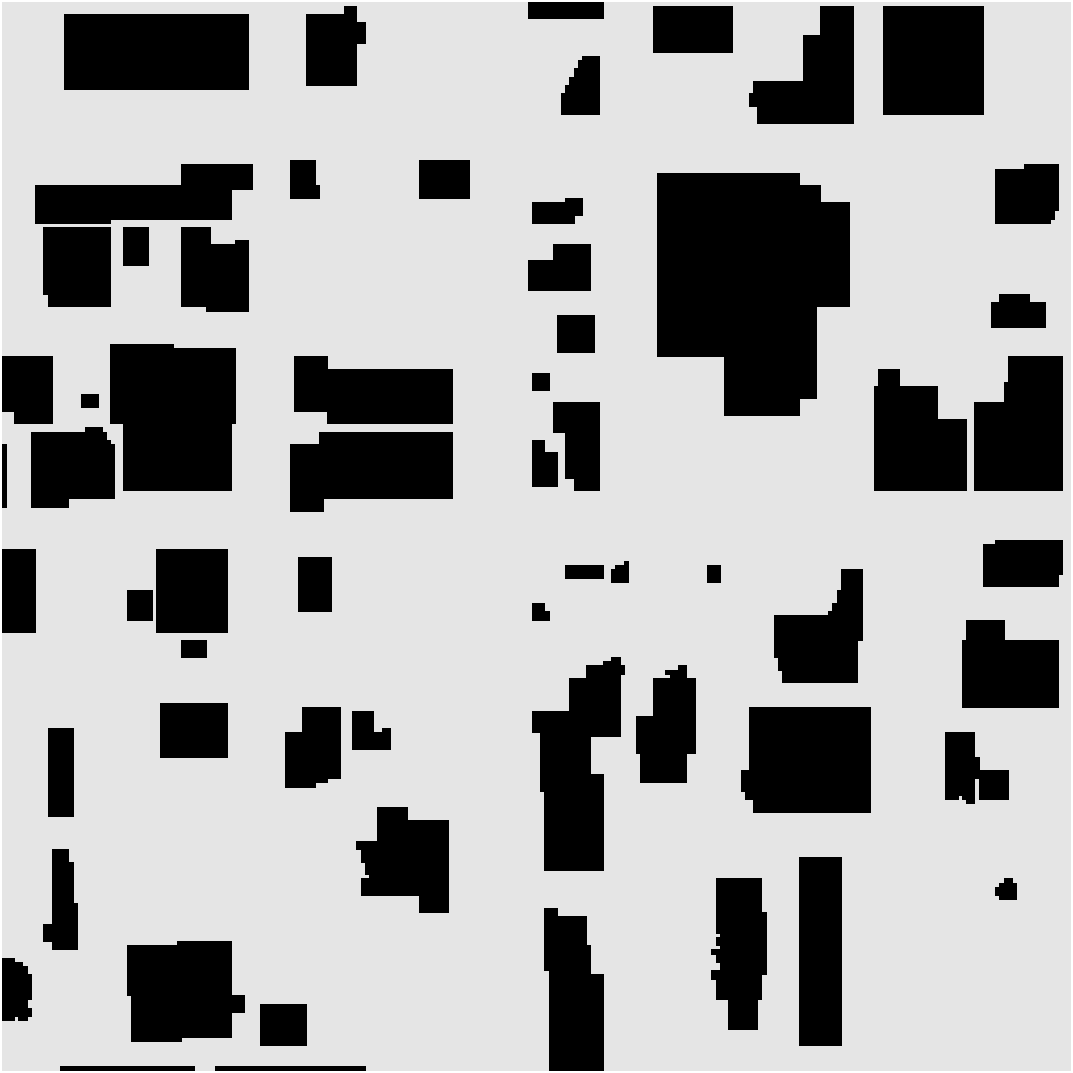
\includegraphics[width=2.1cm]{Denver_2_256.png}}
  \centerline{C: Denver\_2\_256}
\end{minipage}
\hfill
\begin{minipage}{.24\linewidth}
  \centerline{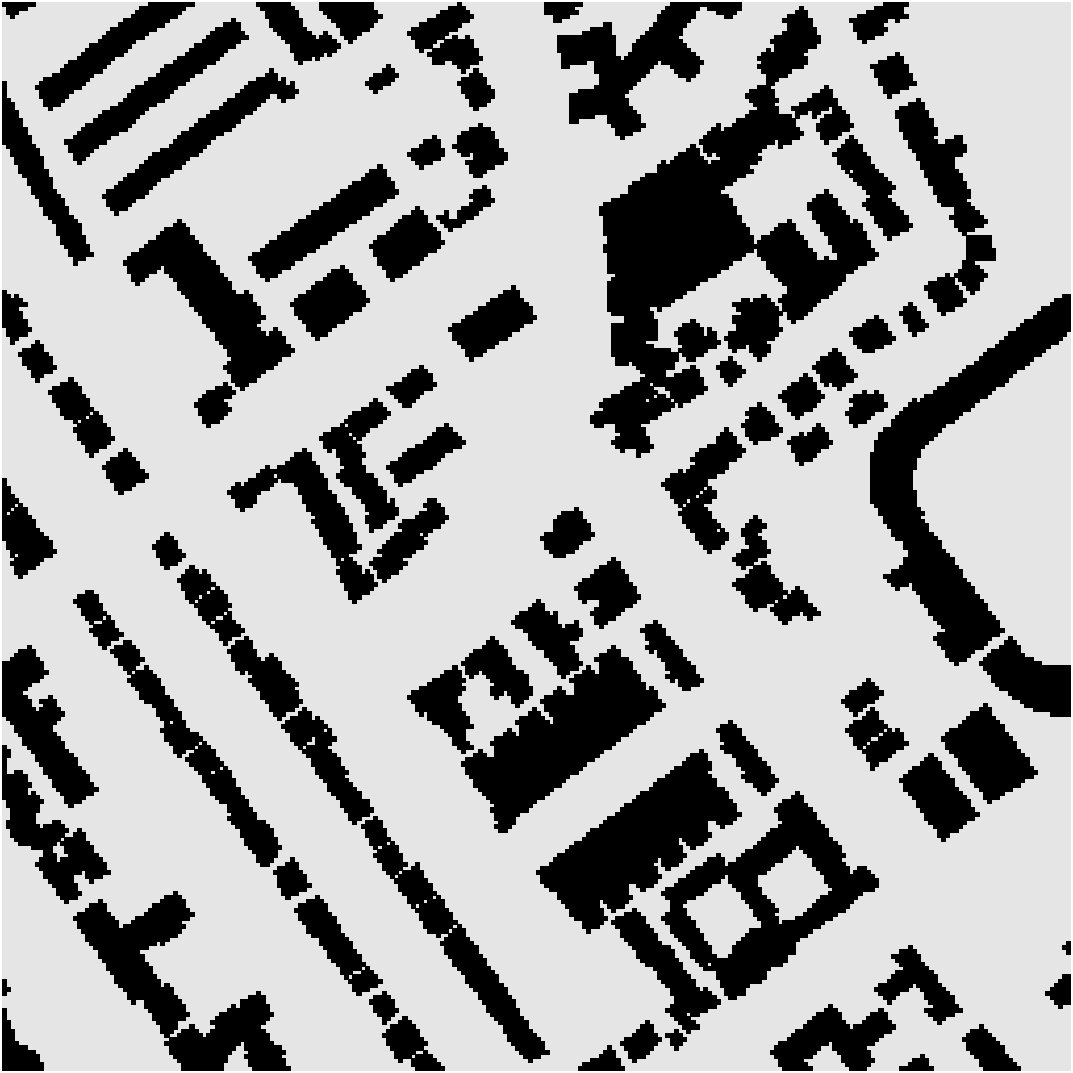
\includegraphics[width=2.1cm]{London_2_256.png}}
  \centerline{D: London\_2\_256}
\end{minipage}
\vfill
\vspace{0.2cm}
\begin{minipage}{.24\linewidth}
  \centerline{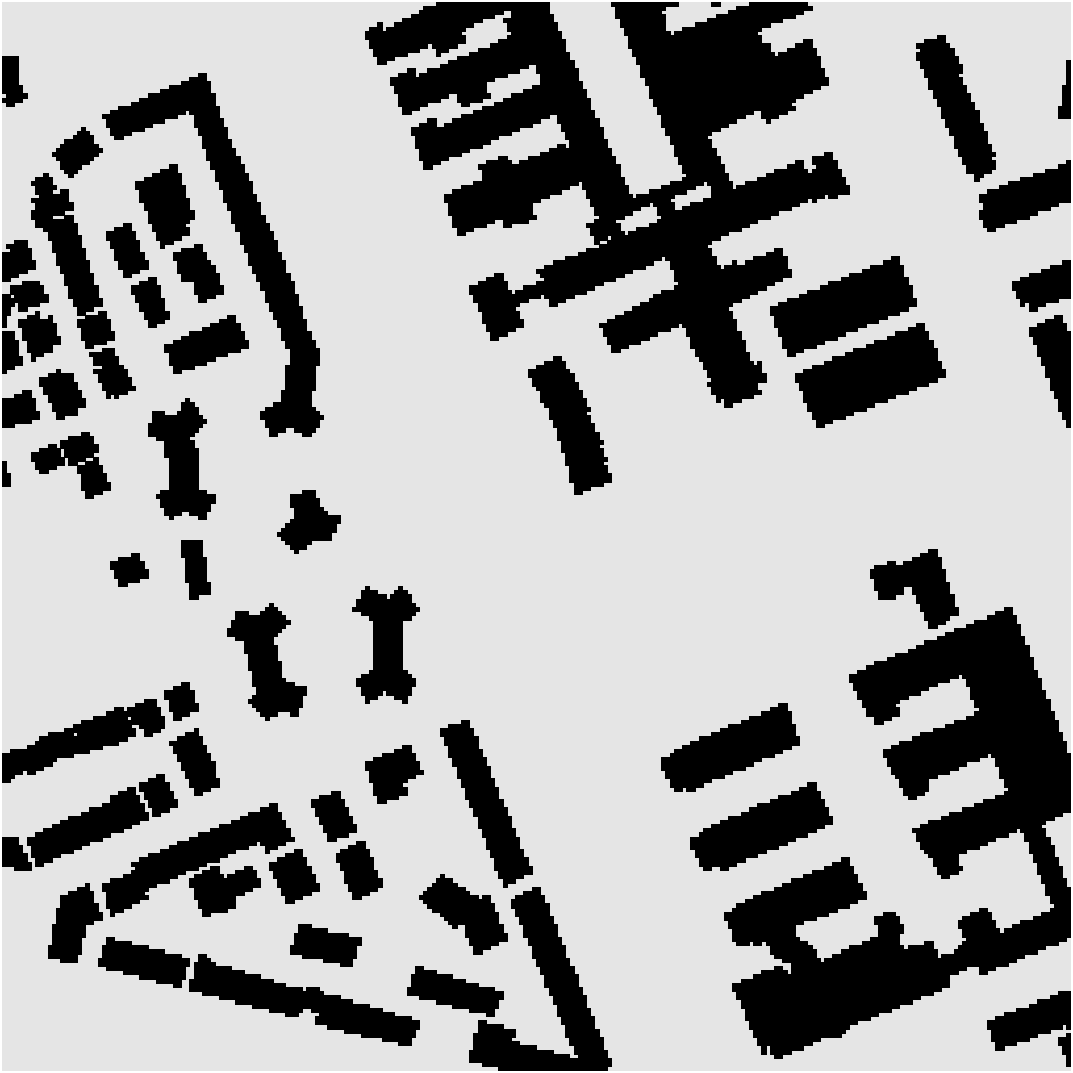
\includegraphics[width=2.1cm]{Milan_2_256.png}}
  \centerline{E: Milan\_2\_256}
\end{minipage}
\hfill
\begin{minipage}{.24\linewidth}
  \centerline{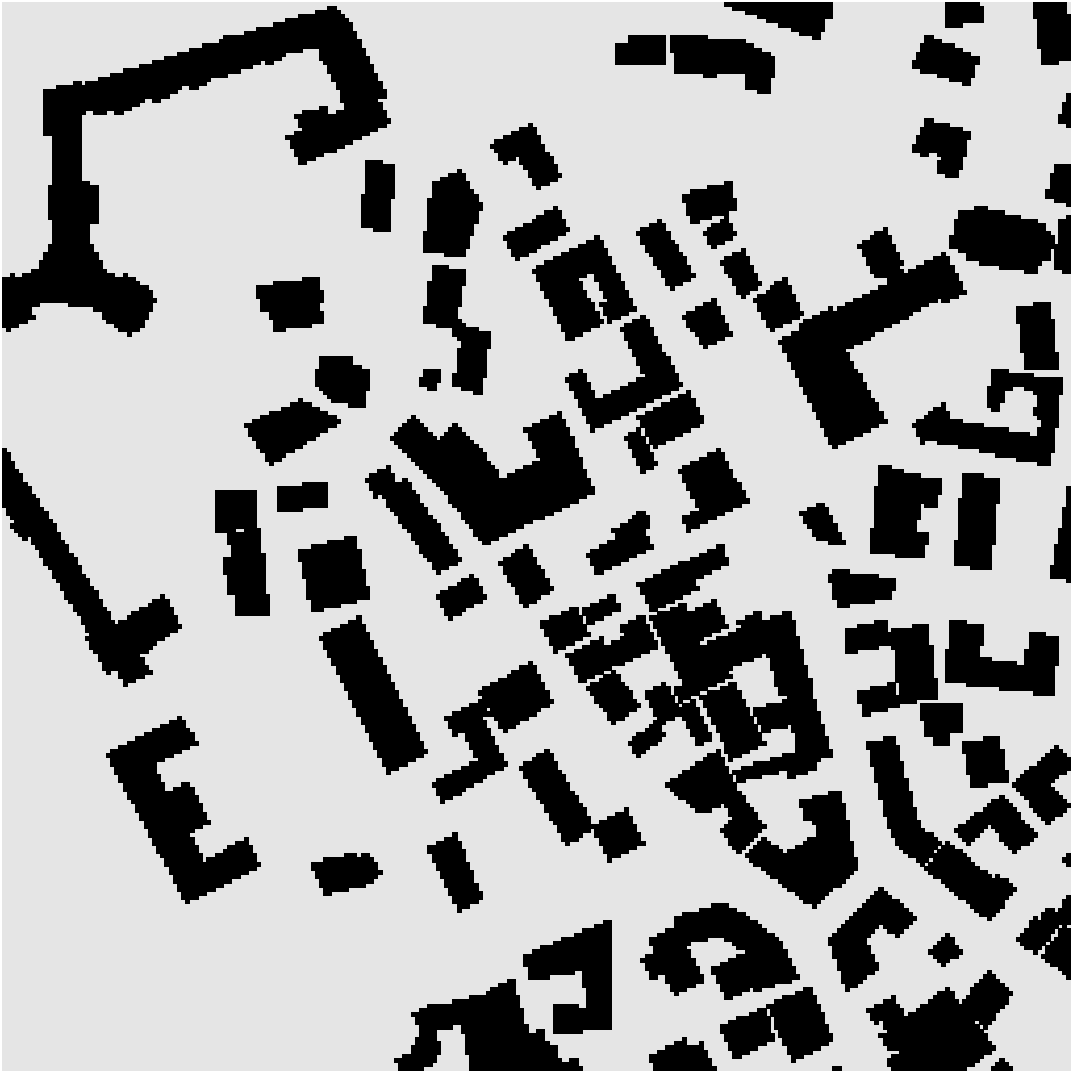
\includegraphics[width=2.1cm]{Moscow_2_256.png}}
  \centerline{F: Moscow\_2\_256}
\end{minipage}
\hfill
\begin{minipage}{.24\linewidth}
  \centerline{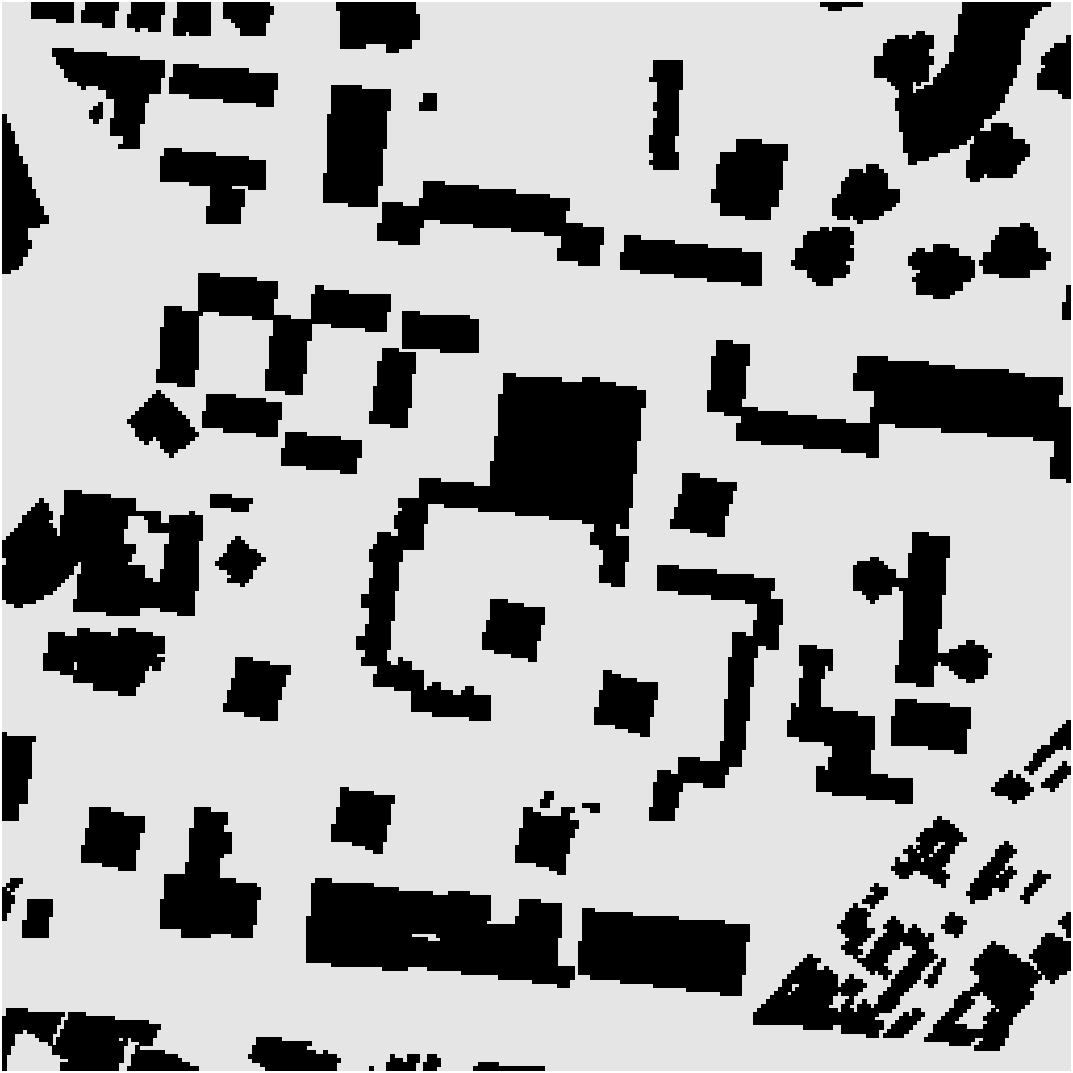
\includegraphics[width=2.1cm]{Paris_0_256.png}}
  \centerline{G: Paris\_0\_256}
\end{minipage}
\hfill
\begin{minipage}{.24\linewidth}
  \centerline{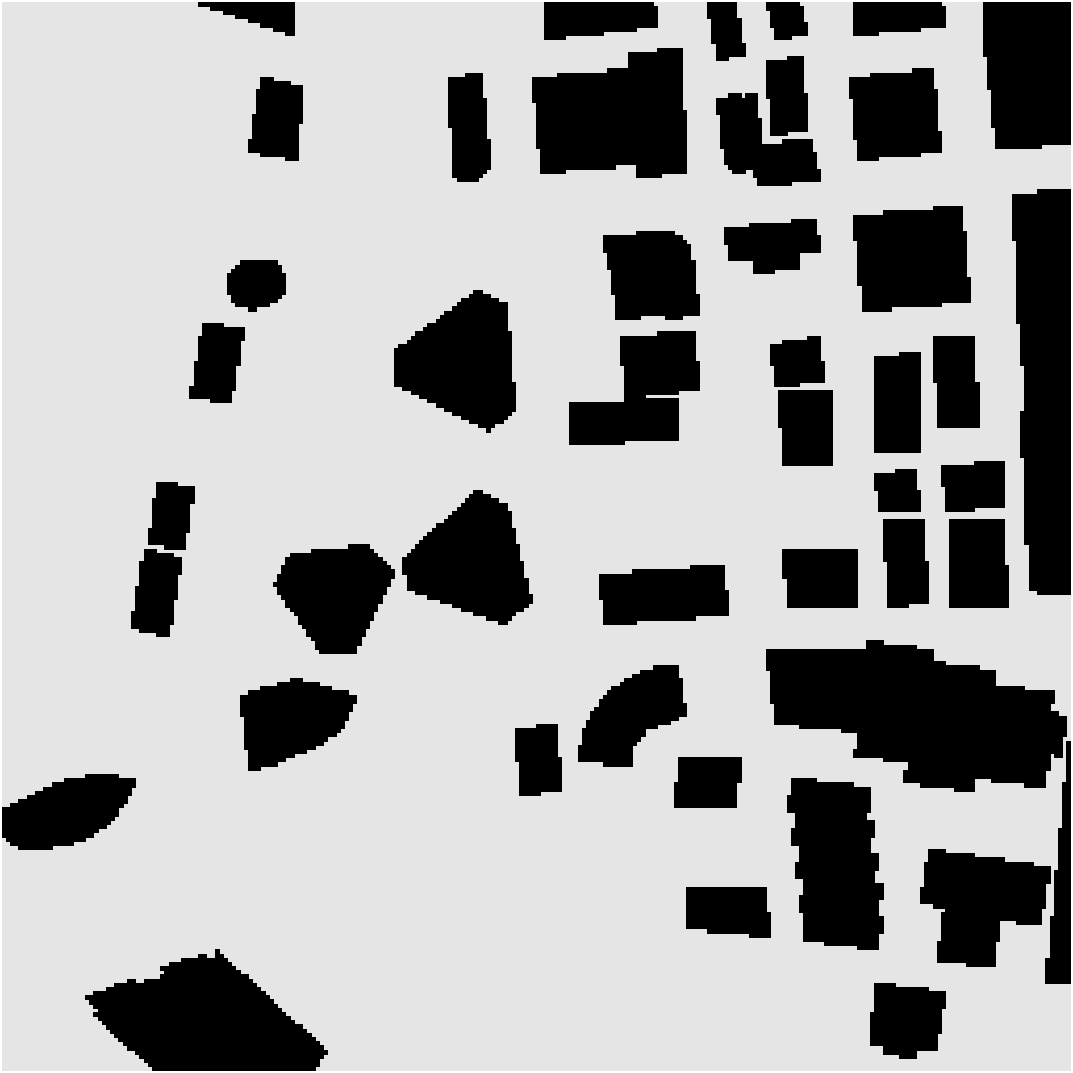
\includegraphics[width=2.1cm]{Sydney_1_256.png}}
  \centerline{H: Sydney\_1\_256}
\end{minipage}
\vfill

\caption{These figures showcase eight grid maps from \cite{sturtevant2012benchmarks} utilized in the comparison with other algorithms. The size of each map is 256$\times$256. In these maps of city streets, grey areas represent passable areas, while black areas represent unpassable areas. }
\label{city_maps}
\end{figure}

\section{Results}
\label{Results}

In this section, we delve into a detailed examination of our algorithm's performance, comparing it with other distinctive topology path planning methods. The first subsection provides insights into the construction of the tangent graph. The second section is about comparison with other algorithms. To ensure a fair comparison, we utilize the implementations provided by the respective authors. There are other algorithms that are worth comparing, such as TARRT*\cite{19} and Kuderer's algorithm\cite{kuderer2014online}, but we found no source code for them. Thus our method is compared with HA*, HTheta*, and RHCF, focusing on the time cost as the required number of paths and the scale of the map increases. Path length comparisons for each method are also conducted, revealing [insert findings here]. HA* and HTheta* are H-signature-based algorithms \footnote{https://github.com/subh83/DOSL}, while RHCF is a Voronoi graph-based algorithm \footnote{https://github.com/srl-freiburg/srl\_rhcf\_planner}; more details about these methods can be found in Section \ref{RelatedWork}. To foster further research within the community, we have made the source code of our proposed algorithm publicly accessible\footnote{https://joeyao-bit.github.io/posts/2023/09/07/}.

The experiments are conducted using a well-known grid map dataset \cite{sturtevant2012benchmarks} \footnote{https://movingai.com/benchmarks/grids.html}. City maps from the dataset are selected for their high obstacle density, allowing the generation of hundreds of topologically distinctive paths, providing ample space for each method to demonstrate its capability. For each map, 100 start and target combinations are randomly sampled as inputs for path planning. To study how method performance changes with an increasing map scale, raw maps are magnified to create larger maps. The magnification ranges from 1.0 to 4.0 (including 1.0, 1.1, 1.2, 1.3, 1.4, 1.5, 1.8, 2.0, 2.5, 3.0, 3.5, 4.0 specifically), resulting in map scales from 256$\times$256 to 1024$\times$1024. Experiments were conducted on a laptop running Ubuntu 20.04, equipped with a Ryzen 7 5800h (3.2GHz) CPU and 16GB of memory.

To showcase the methods' capability to find a substantial number of topologically distinctive paths, we set all methods to find paths ranging from 10 to 400 (including 10, 20, 30, 40, 50, 80, 120, 160, 200, 250, 300, 350, 400 specifically). For HA* and HTheta*, their success rate drops to less than 10\% when attempting to find 200 topologically distinctive paths, so we set the maximum number of required paths for them to 200 to reduce the overall time cost of the experiment.


\subsection{Construction of tangent graph}

\begin{figure}[t] \scriptsize
%\begin{tabular}{cc}
\begin{minipage}{.48\linewidth}
  \centerline{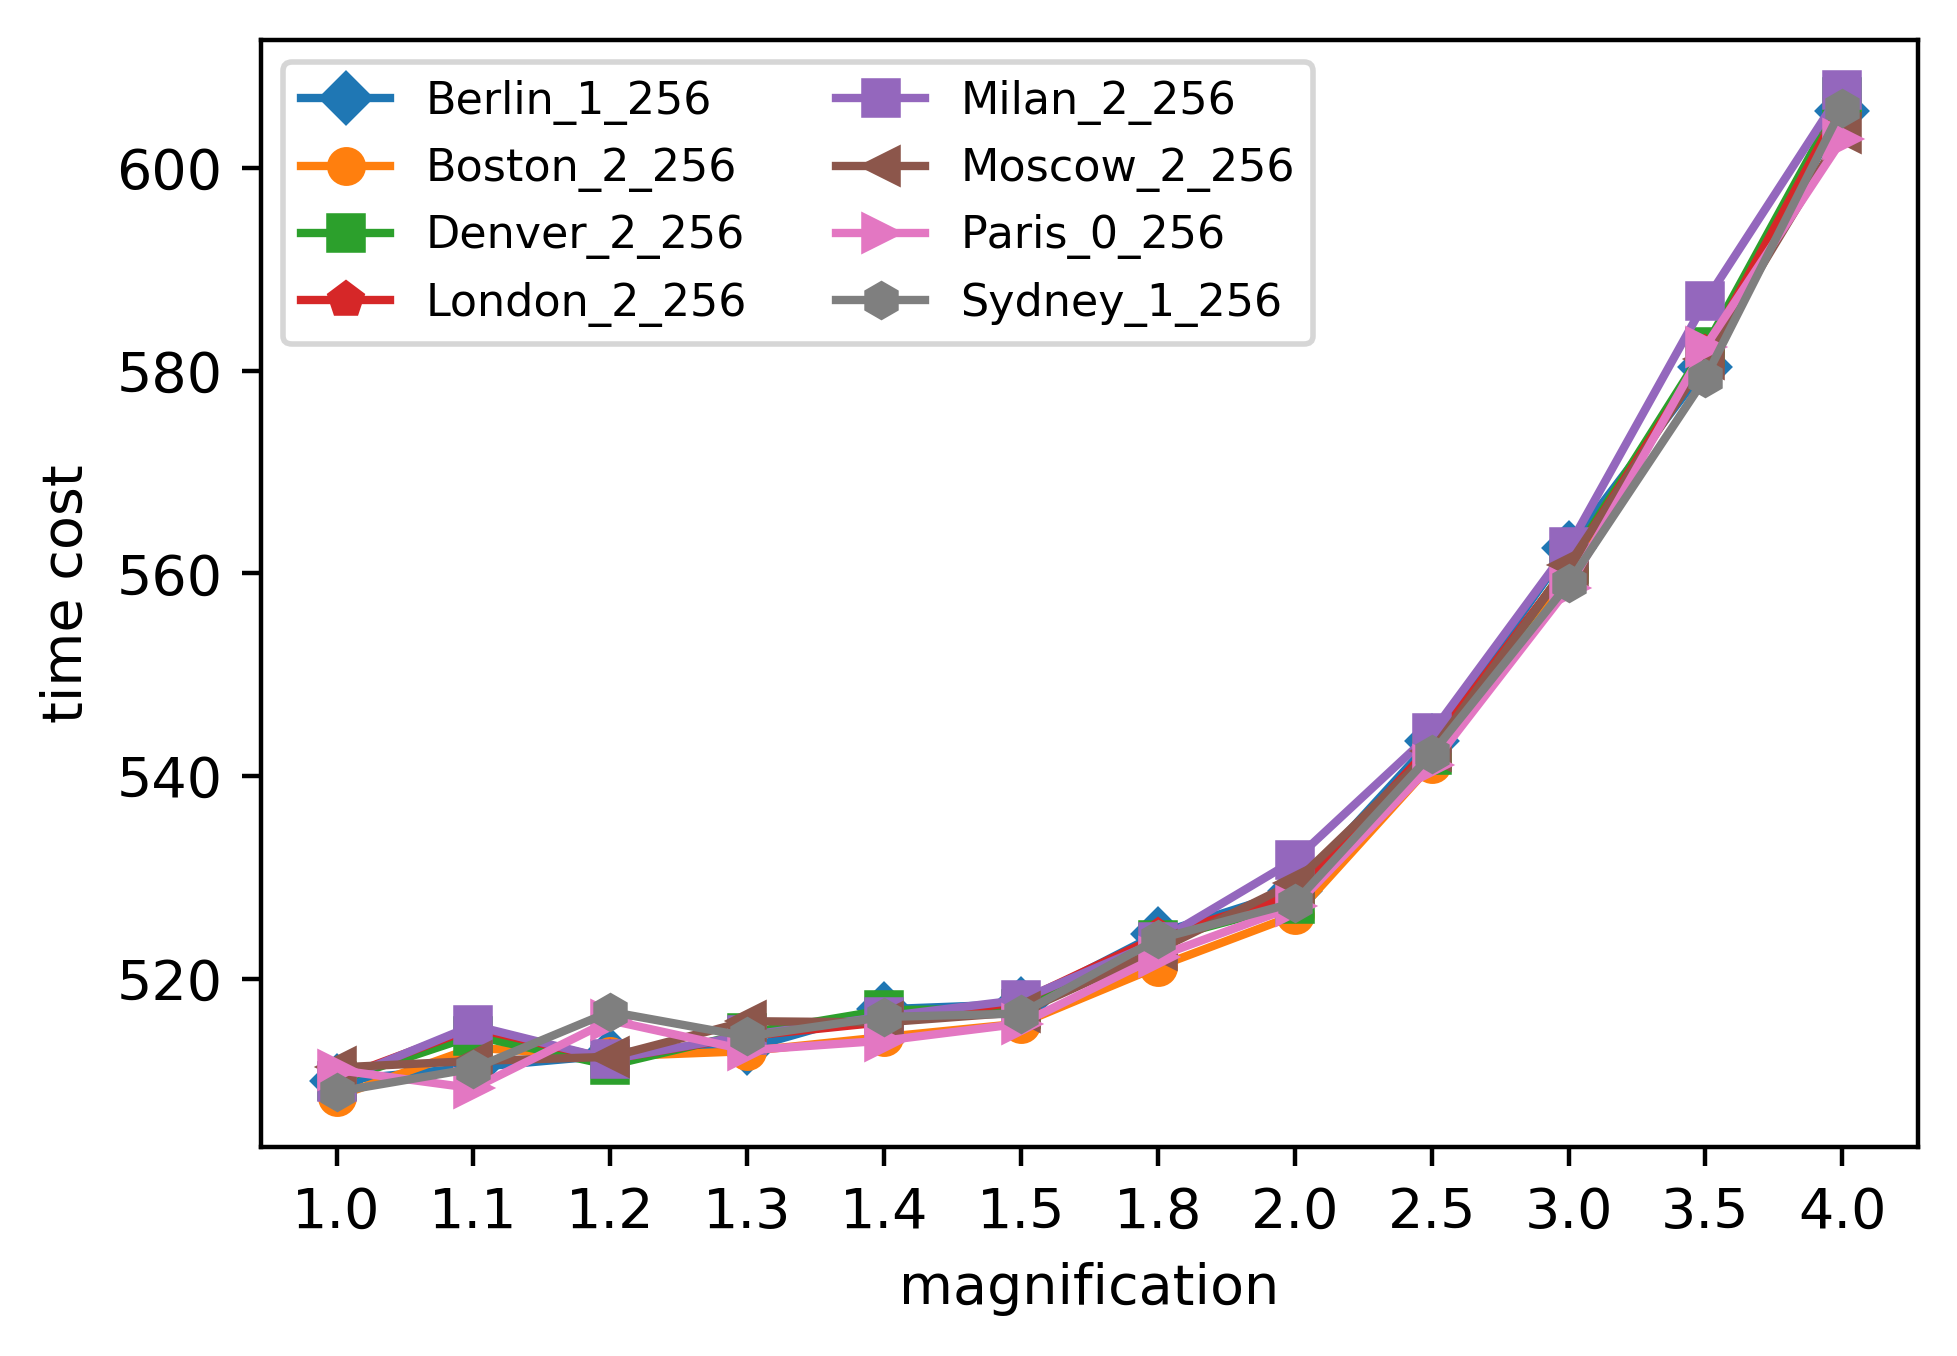
\includegraphics[width=4.6cm]{pre_time_cost.png}}
  \centerline{A: time cost comparison}
\end{minipage}
\hfill
\begin{minipage}{.48\linewidth}
  \centerline{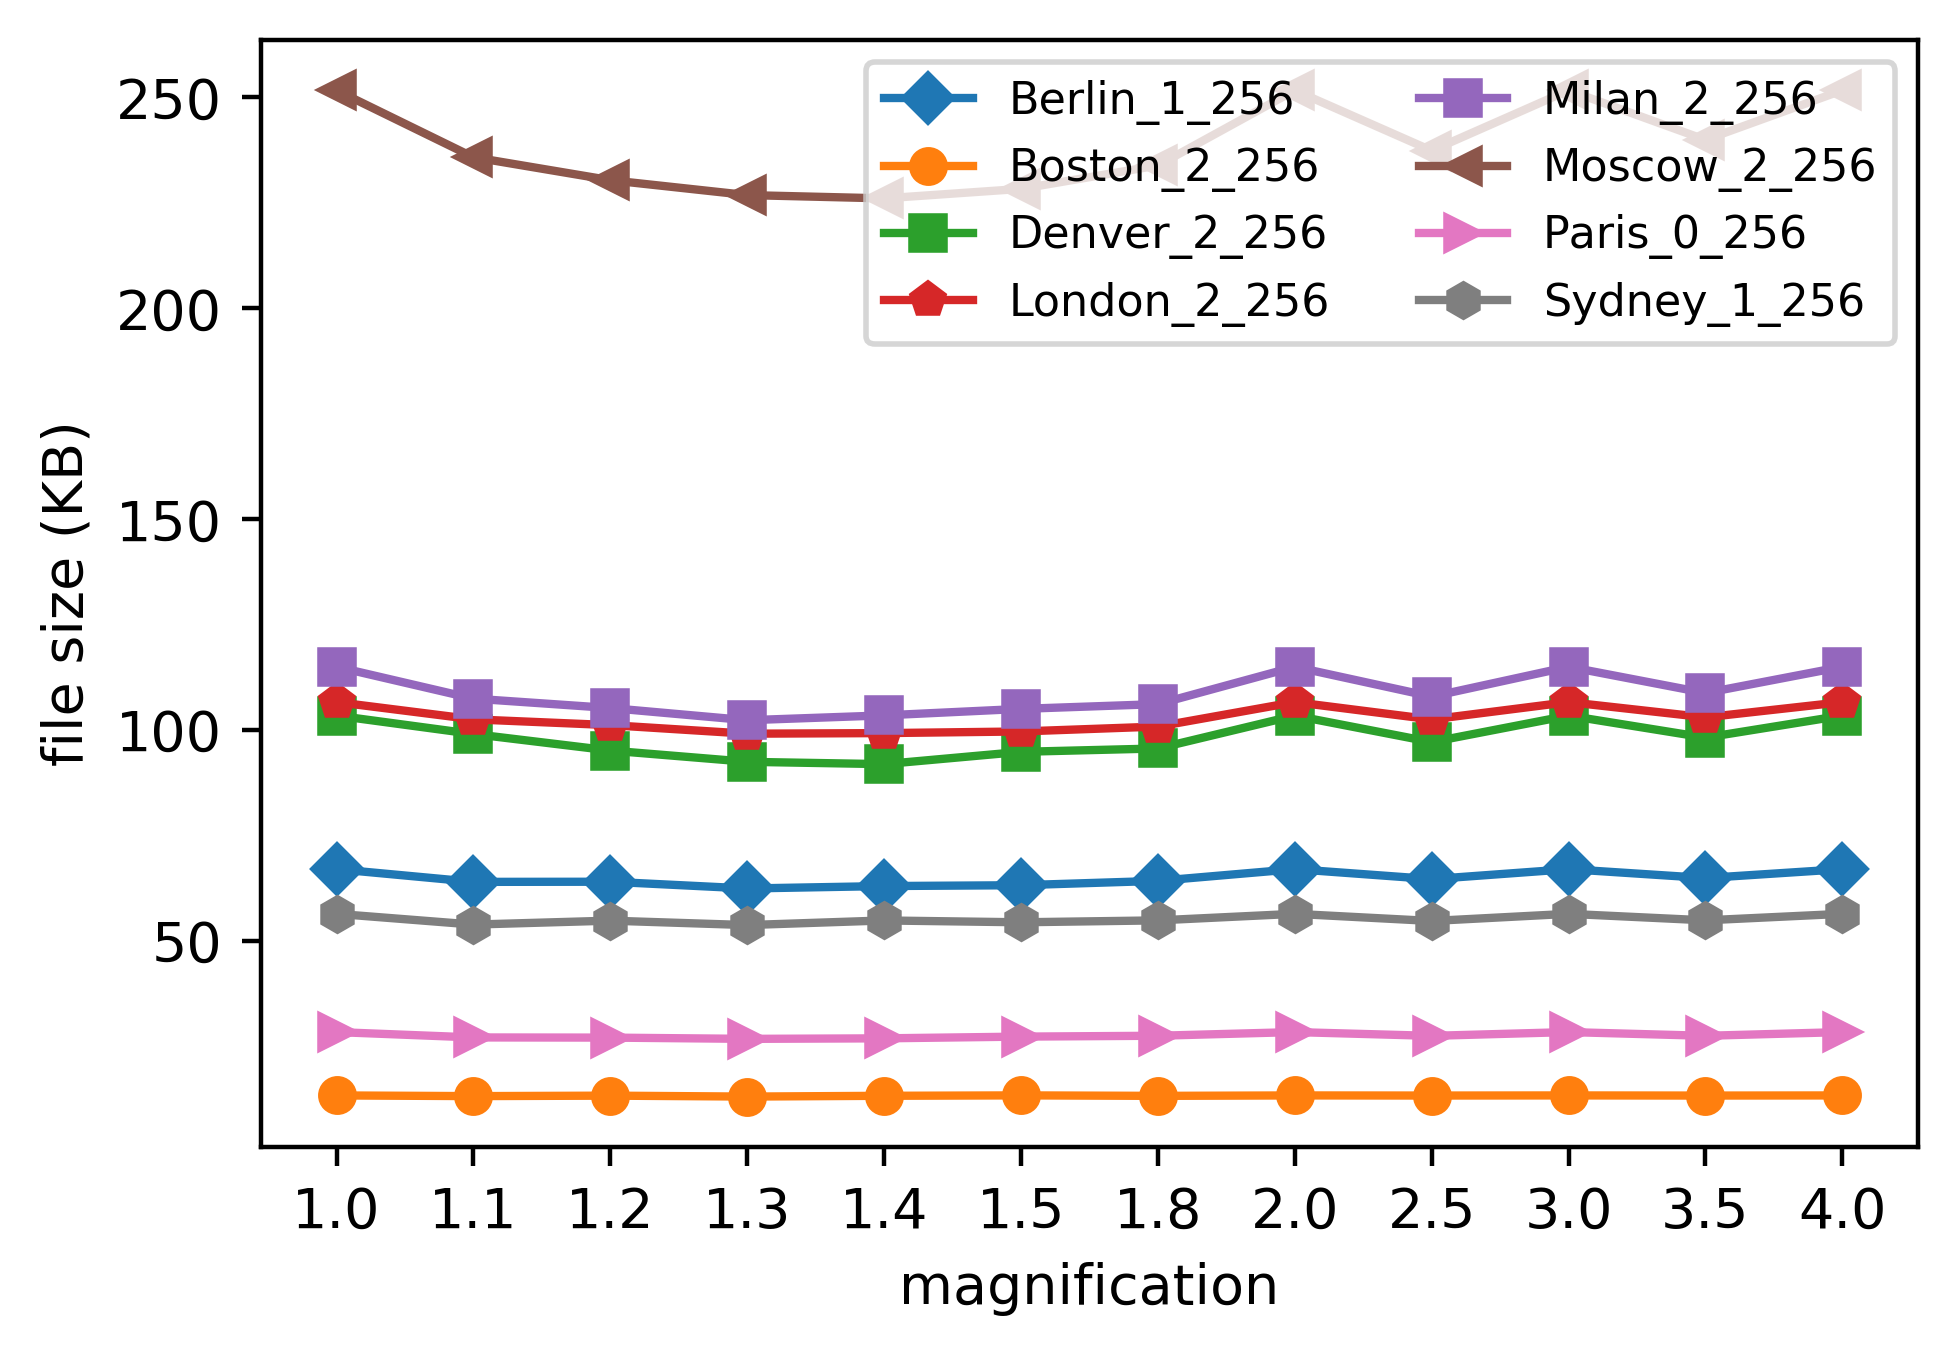
\includegraphics[width=4.6cm]{pre_file_size.png}}
  \centerline{B: time cost comparison}
\end{minipage}
\vfill

\caption{These two figures present comprehensive data pertaining to the tangent graph detection process of our method. The data includes information on time cost and file size to save the graph, encompassing various magnifications of the map. Figure 1 details the time cost across different magnifications, while Figure 2 provides insights into the corresponding file sizes.}
\label{precomputation_data}
\end{figure}

In this section, we elaborate on the construction of the tangent graph for the aforementioned eight maps across various magnifications. The associated data, including time cost and file size, is summarized in Fig \ref{precomputation_data}.

The construction of the tangent graph for nearly all maps is completed in approximately 0.5 seconds, indicating nearly real-time updates. Notably, the time cost exhibits a gradual increase as the scale magnifies. Specifically, when the map's scale increases fourfold, the time cost only experiences a 20\% increment.

The file size required to store the tangent graph for these maps ranges from 10KB to 300KB, demonstrating a manageable size for ordinary computing platforms. Importantly, the size of the tangent graph remains stable as the map scale increases. This observation suggests that the tangent graph exhibits insensitivity to variations in map resolution, making it well-suited for real-world maps with high resolutions.


\subsection{Comparison with other methods}
%In this section, we focus on compare our method with other methods, including HA*, HTheta* and RHCF. In practice, distinctive topology path planning have a time cost upper bound, to avoid cost more time than expectation. And if a method finds no all solution within the time bound, it return all solution it have found. So in section, we set the time upper bound to 10s, and apply the success rate to find all solution within time bound as a indicator to evaluate the performance of methods. Essentially, success rate is determine by time cost.

%Moreover, we compare all methods in terms of path length, which is also a very important indicator in path planning. Considering map scale have a siginicant influence on the performance path planning algorithms, we also test the four mentioned methods under map have the same content but scale range from 256*256 to 1024*1024.
    
In this section, our focus centers on the comparative analysis of our method with other prominent approaches, namely HA*, HTheta*, and RHCF. 

In practical applications, topologically distinctive path planning is often constrained by an upper limit on time costs to avoid exceeding expected time constraints. When a method fails to find all solutions within the specified time bound, it returns the solutions it has discovered up to that point. Therefore, in this section, we impose a time upper bound of 10 seconds and employ the success rate – the ability to find all solutions within the time constraint – as an indicative measure for evaluating the performance of the methods. Essentially, the success rate is determined by the time cost incurred.

Furthermore, we conduct a comparative assessment of all methods with respect to path length – a crucial metric in path planning. Recognizing that map scale significantly influences the performance of path planning algorithms, we conduct tests on the four aforementioned methods using maps with identical content but scales ranging from 256$\times$256 to 1024$\times$1024.    
    
\subsubsection{Time cost and success rate}

% total time cost and required path count
\begin{figure*}[t] \scriptsize
%\begin{tabular}{cc}
\begin{minipage}{.245\linewidth}
  \centerline{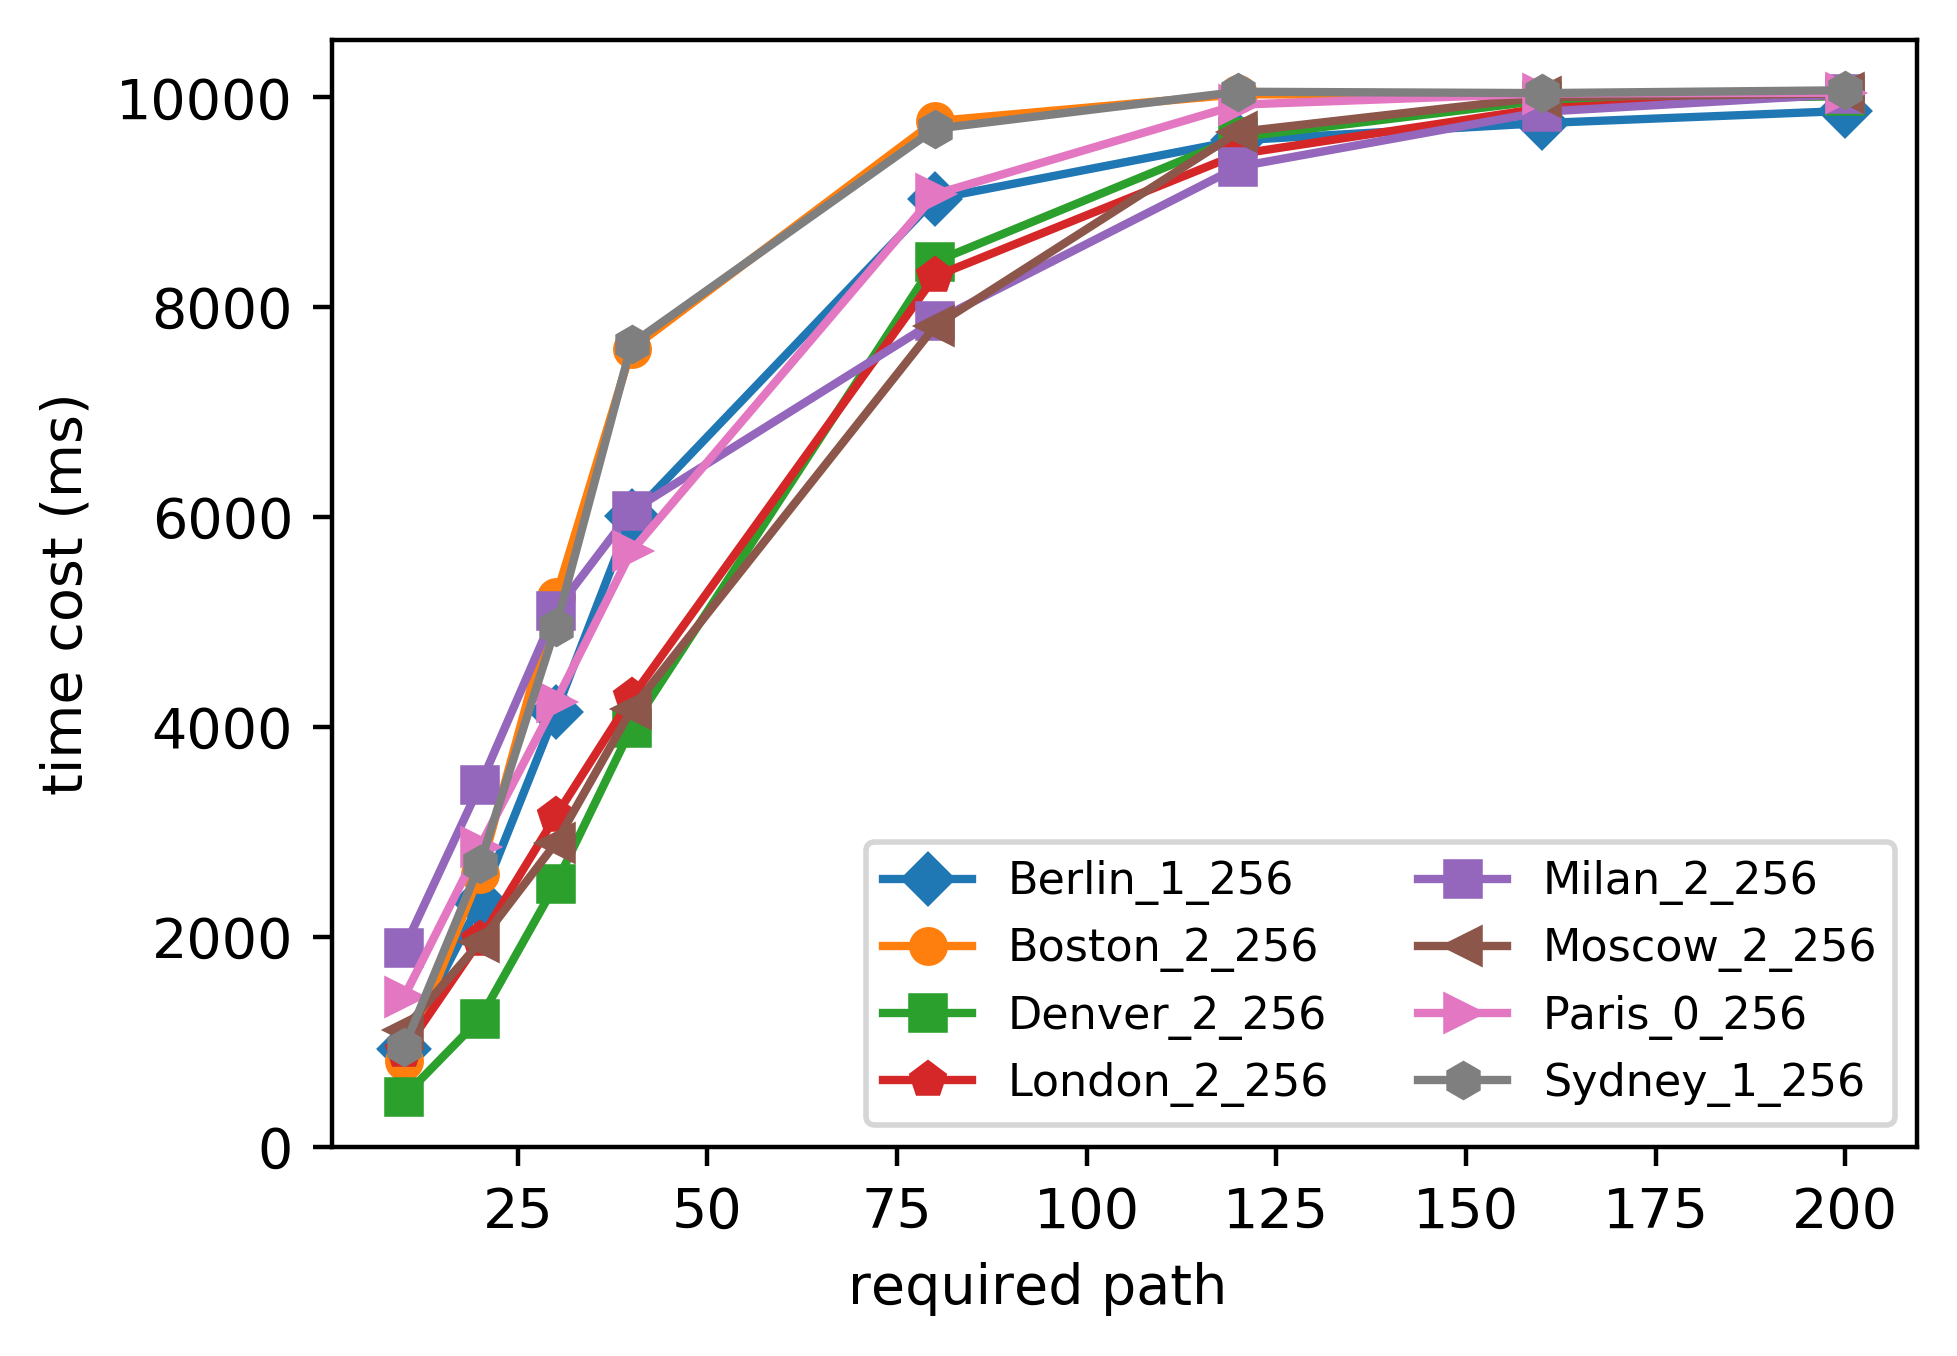
\includegraphics[width=4.6cm]{HsAs_time_and_count.png}}
  \centerline{A: HA*}
\end{minipage}
\hfill
\begin{minipage}{.245\linewidth}
  \centerline{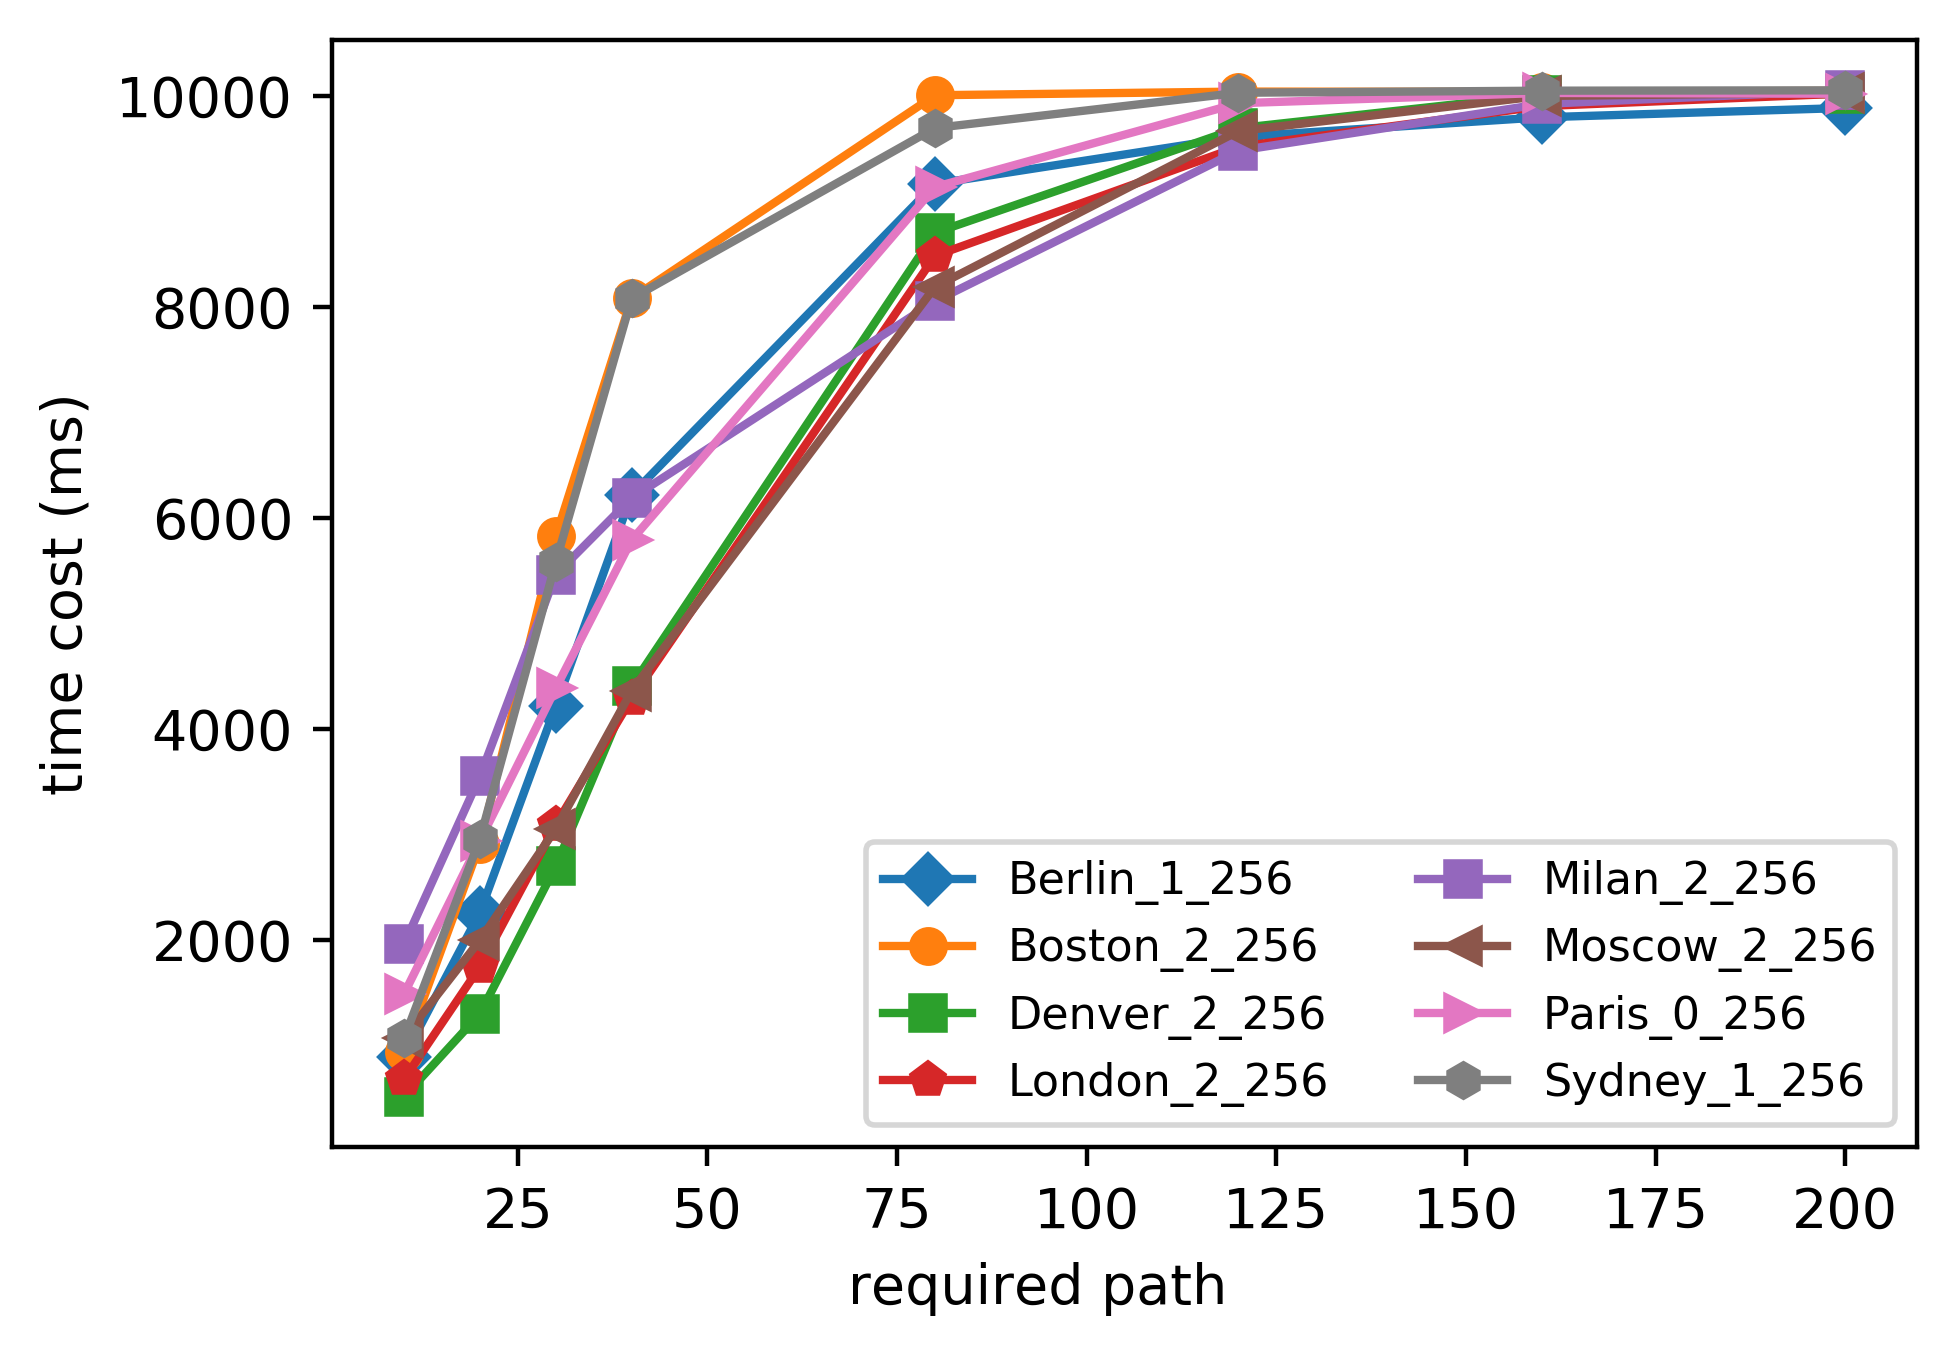
\includegraphics[width=4.6cm]{HsTs_time_and_count.png}}
  \centerline{B: HTheta*}
\end{minipage}
\hfill
\begin{minipage}{.245\linewidth}
  \centerline{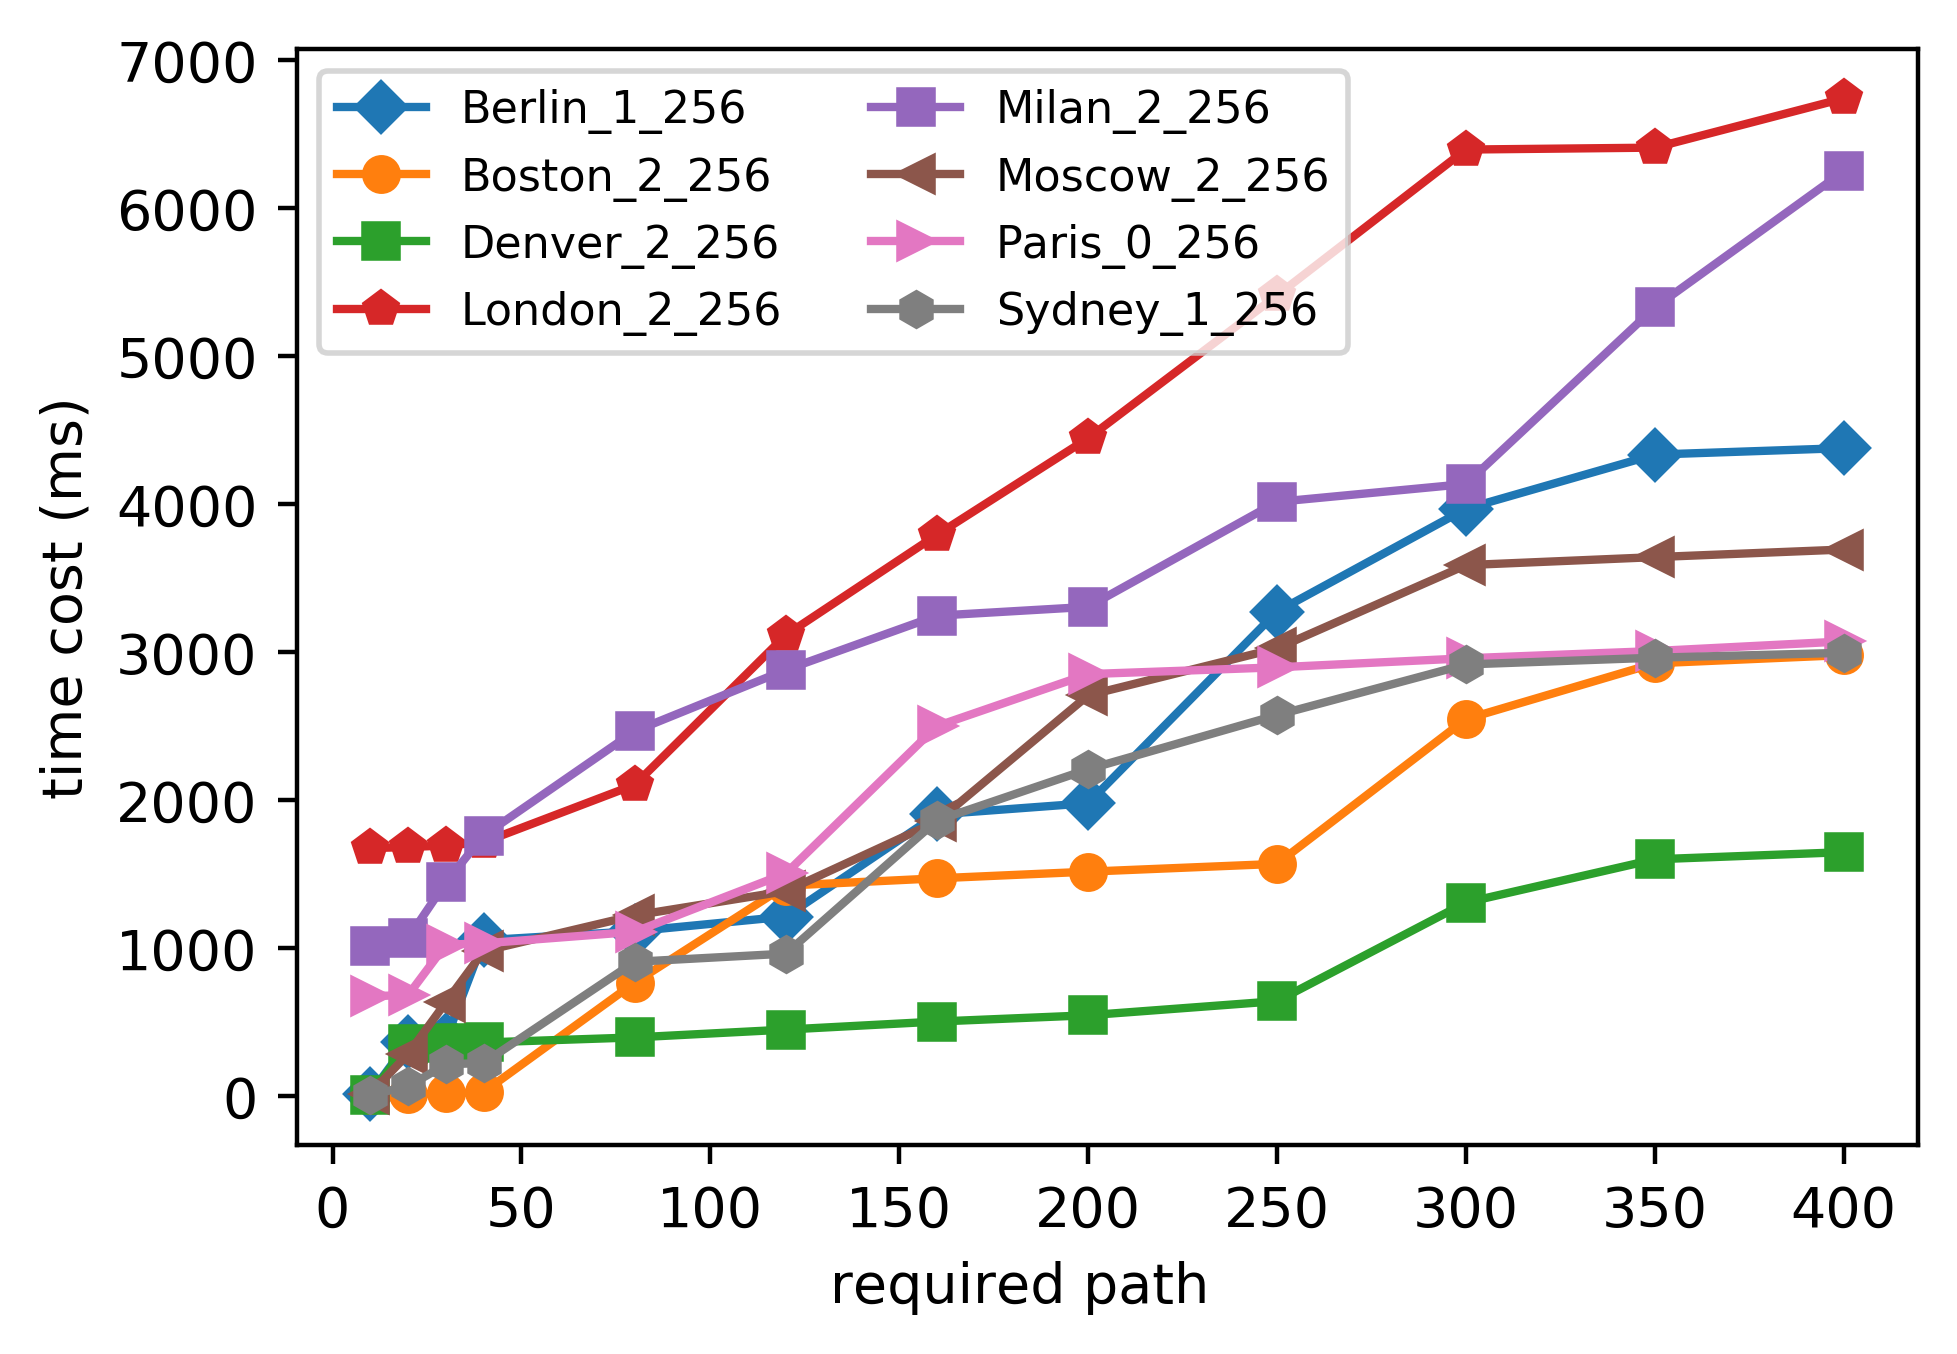
\includegraphics[width=4.6cm]{RHCF_time_and_count.png}}
  \centerline{C: RHCF}
\end{minipage}
\hfill
\begin{minipage}{.245\linewidth}
  \centerline{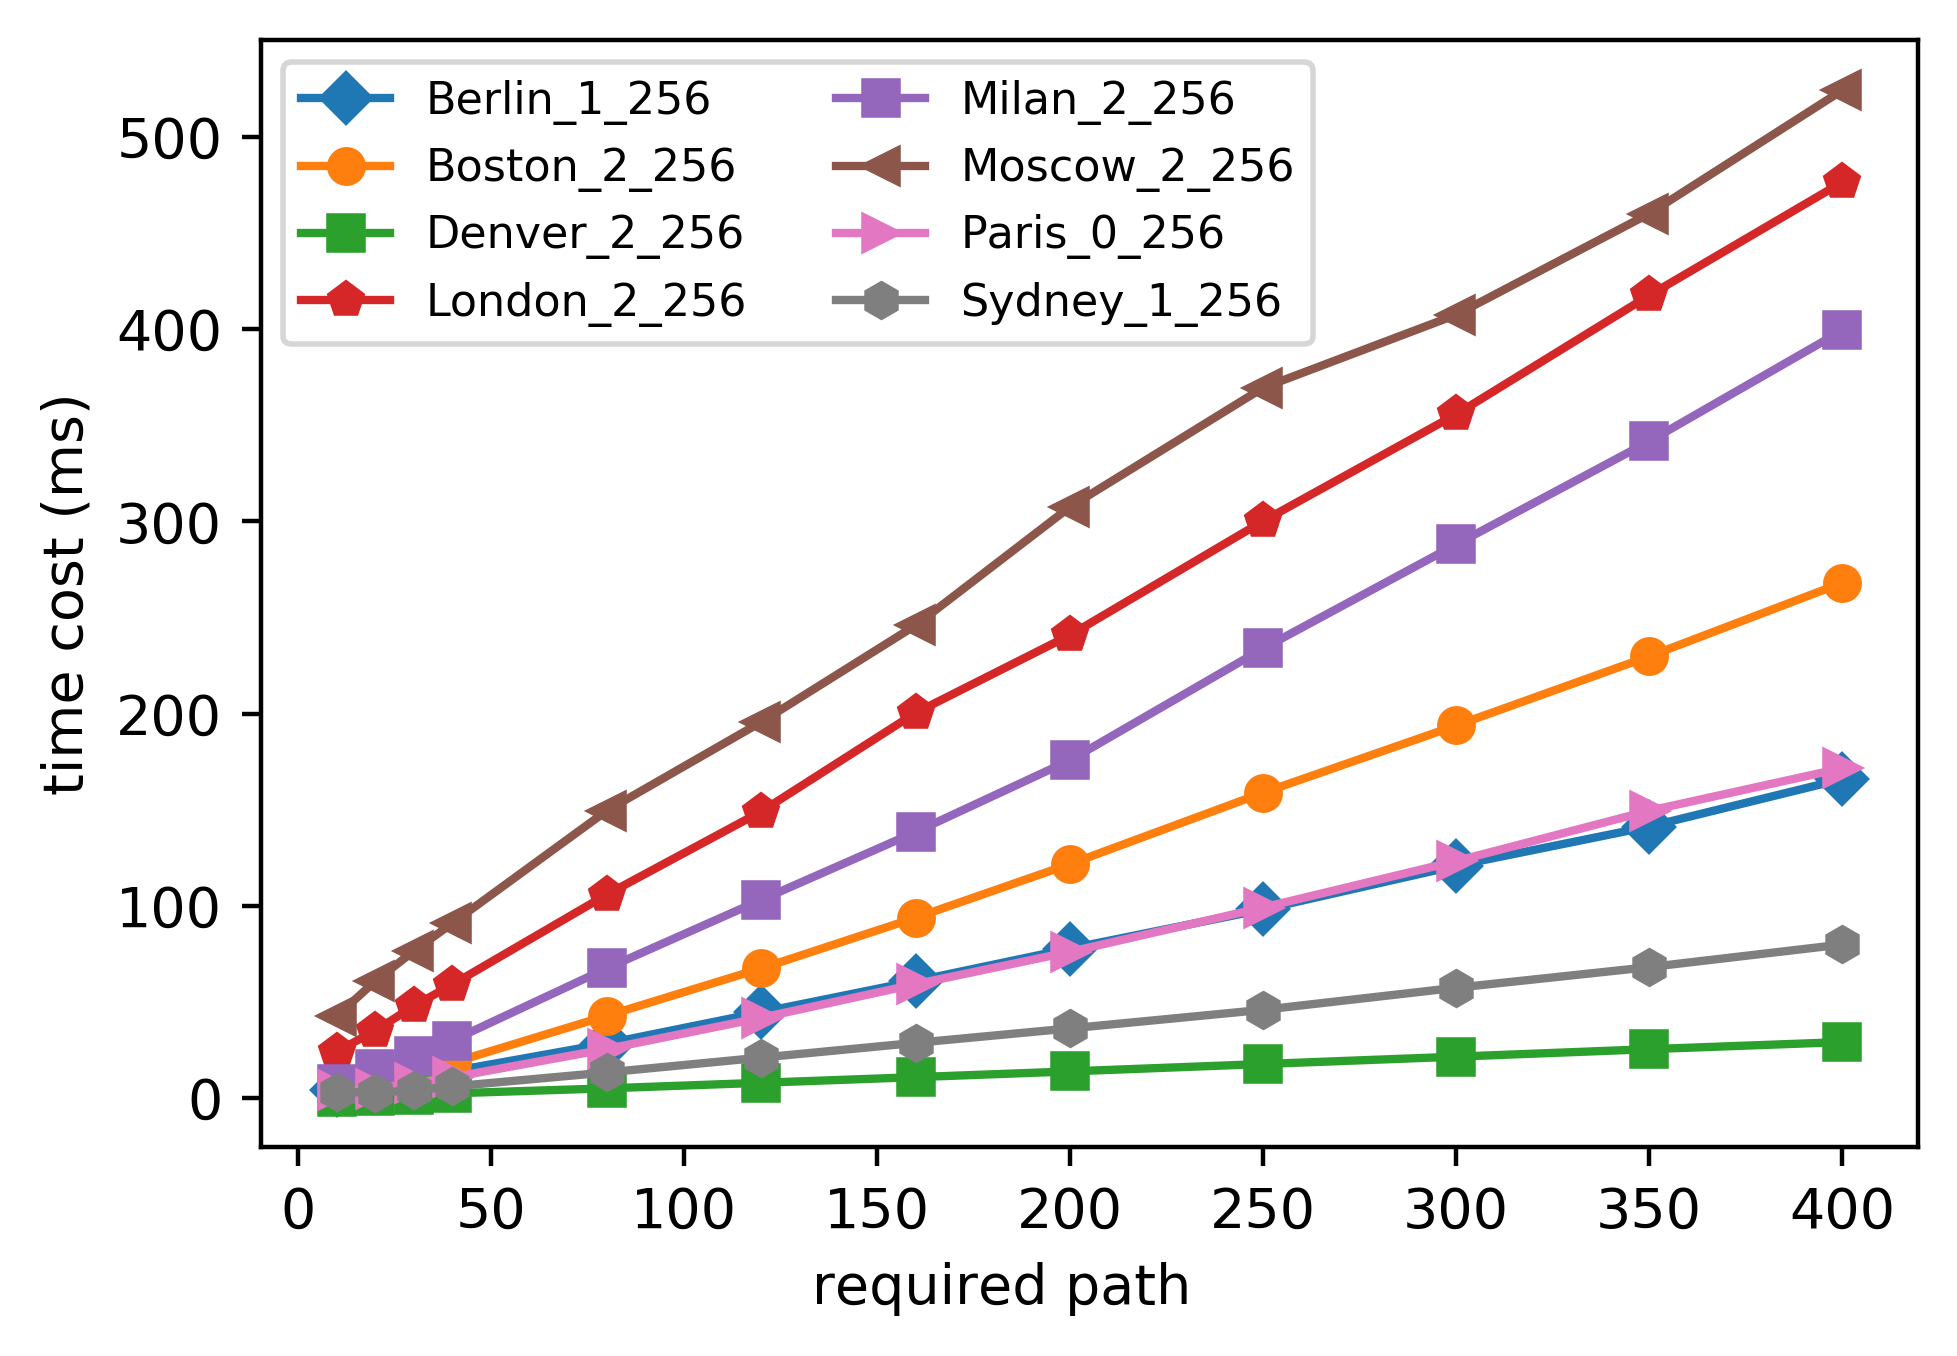
\includegraphics[width=4.6cm]{RJ_time_and_count.png}}
  \centerline{D: Our method}
\end{minipage}
\vfill

\caption{These figures illustrate the mean time cost for finding the required number of paths for each map using all four methods. The magnification for all maps is set to 1.0.}
\label{total_time_cost_and_path_count}
\end{figure*}

% success rate and required path count
\begin{figure*}[t] \scriptsize
%\begin{tabular}{cc}
\begin{minipage}{.245\linewidth}
  \centerline{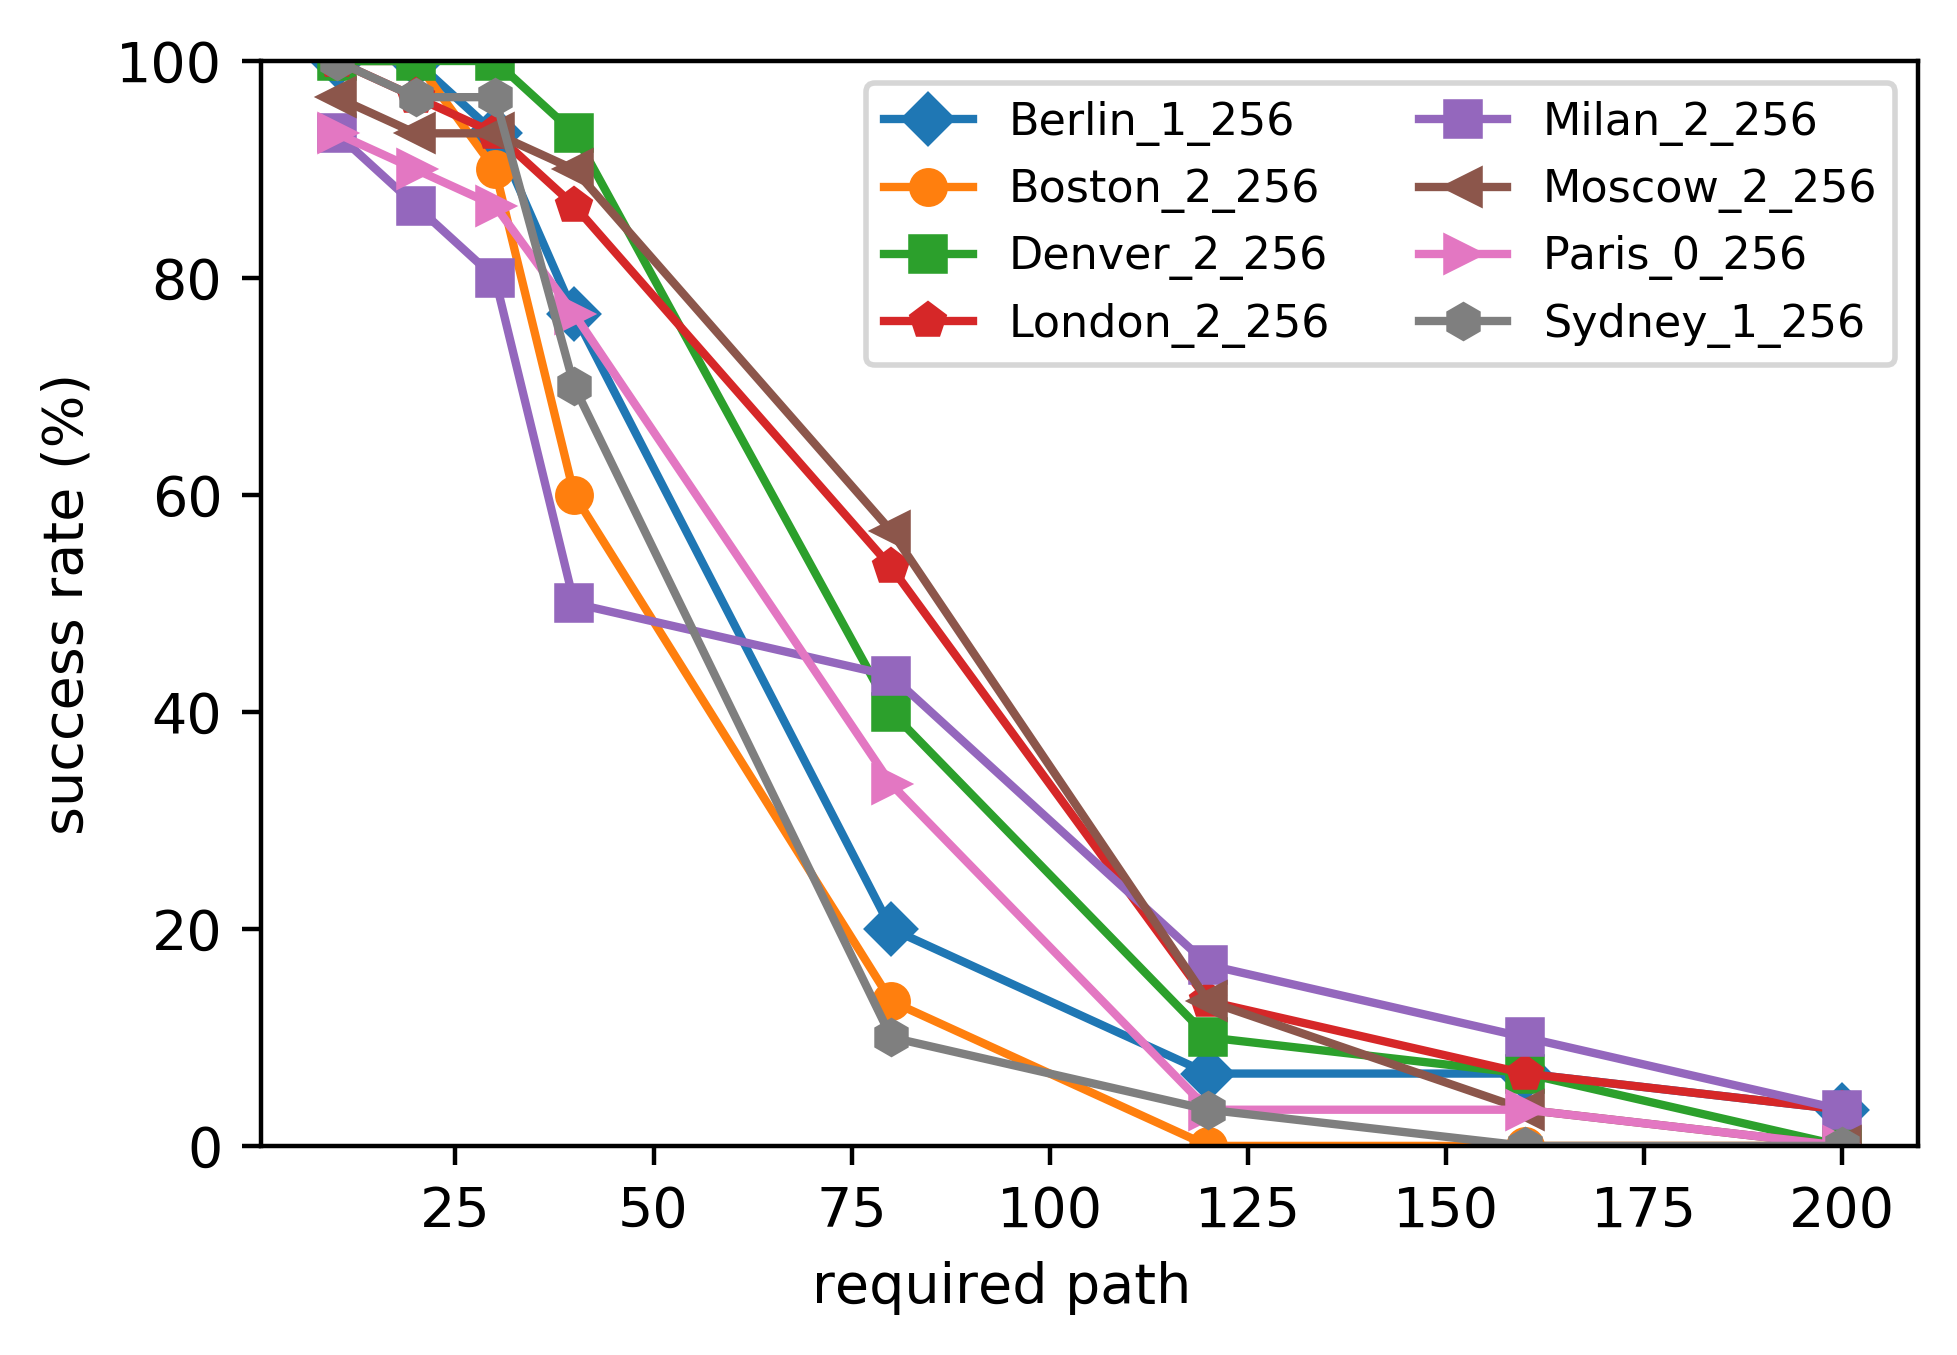
\includegraphics[width=4.6cm]{HsAs_succ_and_count.png}}
  \centerline{A: HA*}
\end{minipage}
\hfill
\begin{minipage}{.245\linewidth}
  \centerline{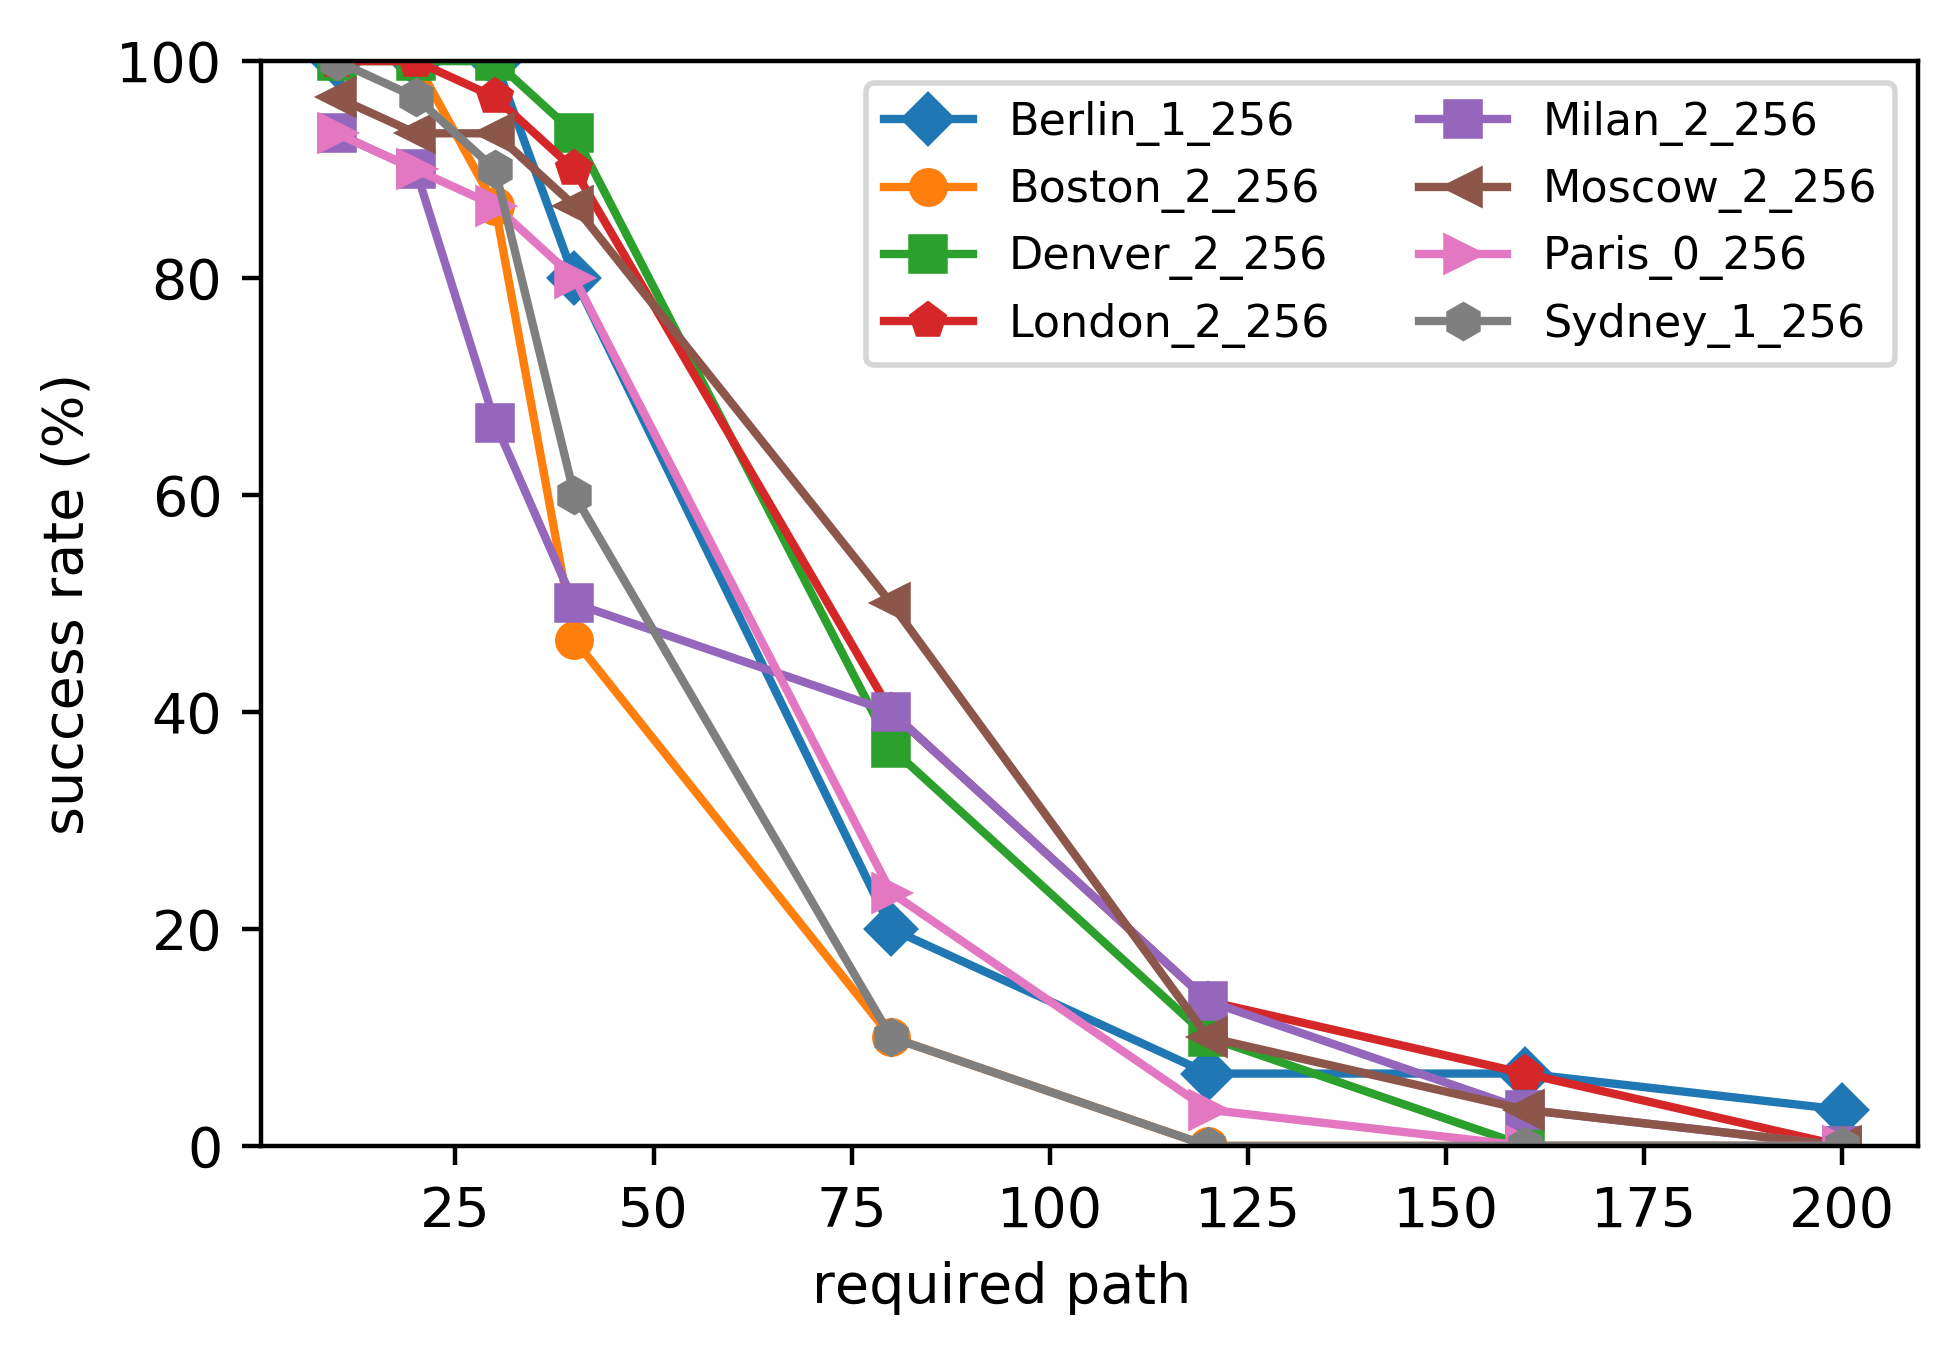
\includegraphics[width=4.6cm]{HsTs_succ_and_count.png}}
  \centerline{B: HTheta*}
\end{minipage}
\hfill
\begin{minipage}{.245\linewidth}
  \centerline{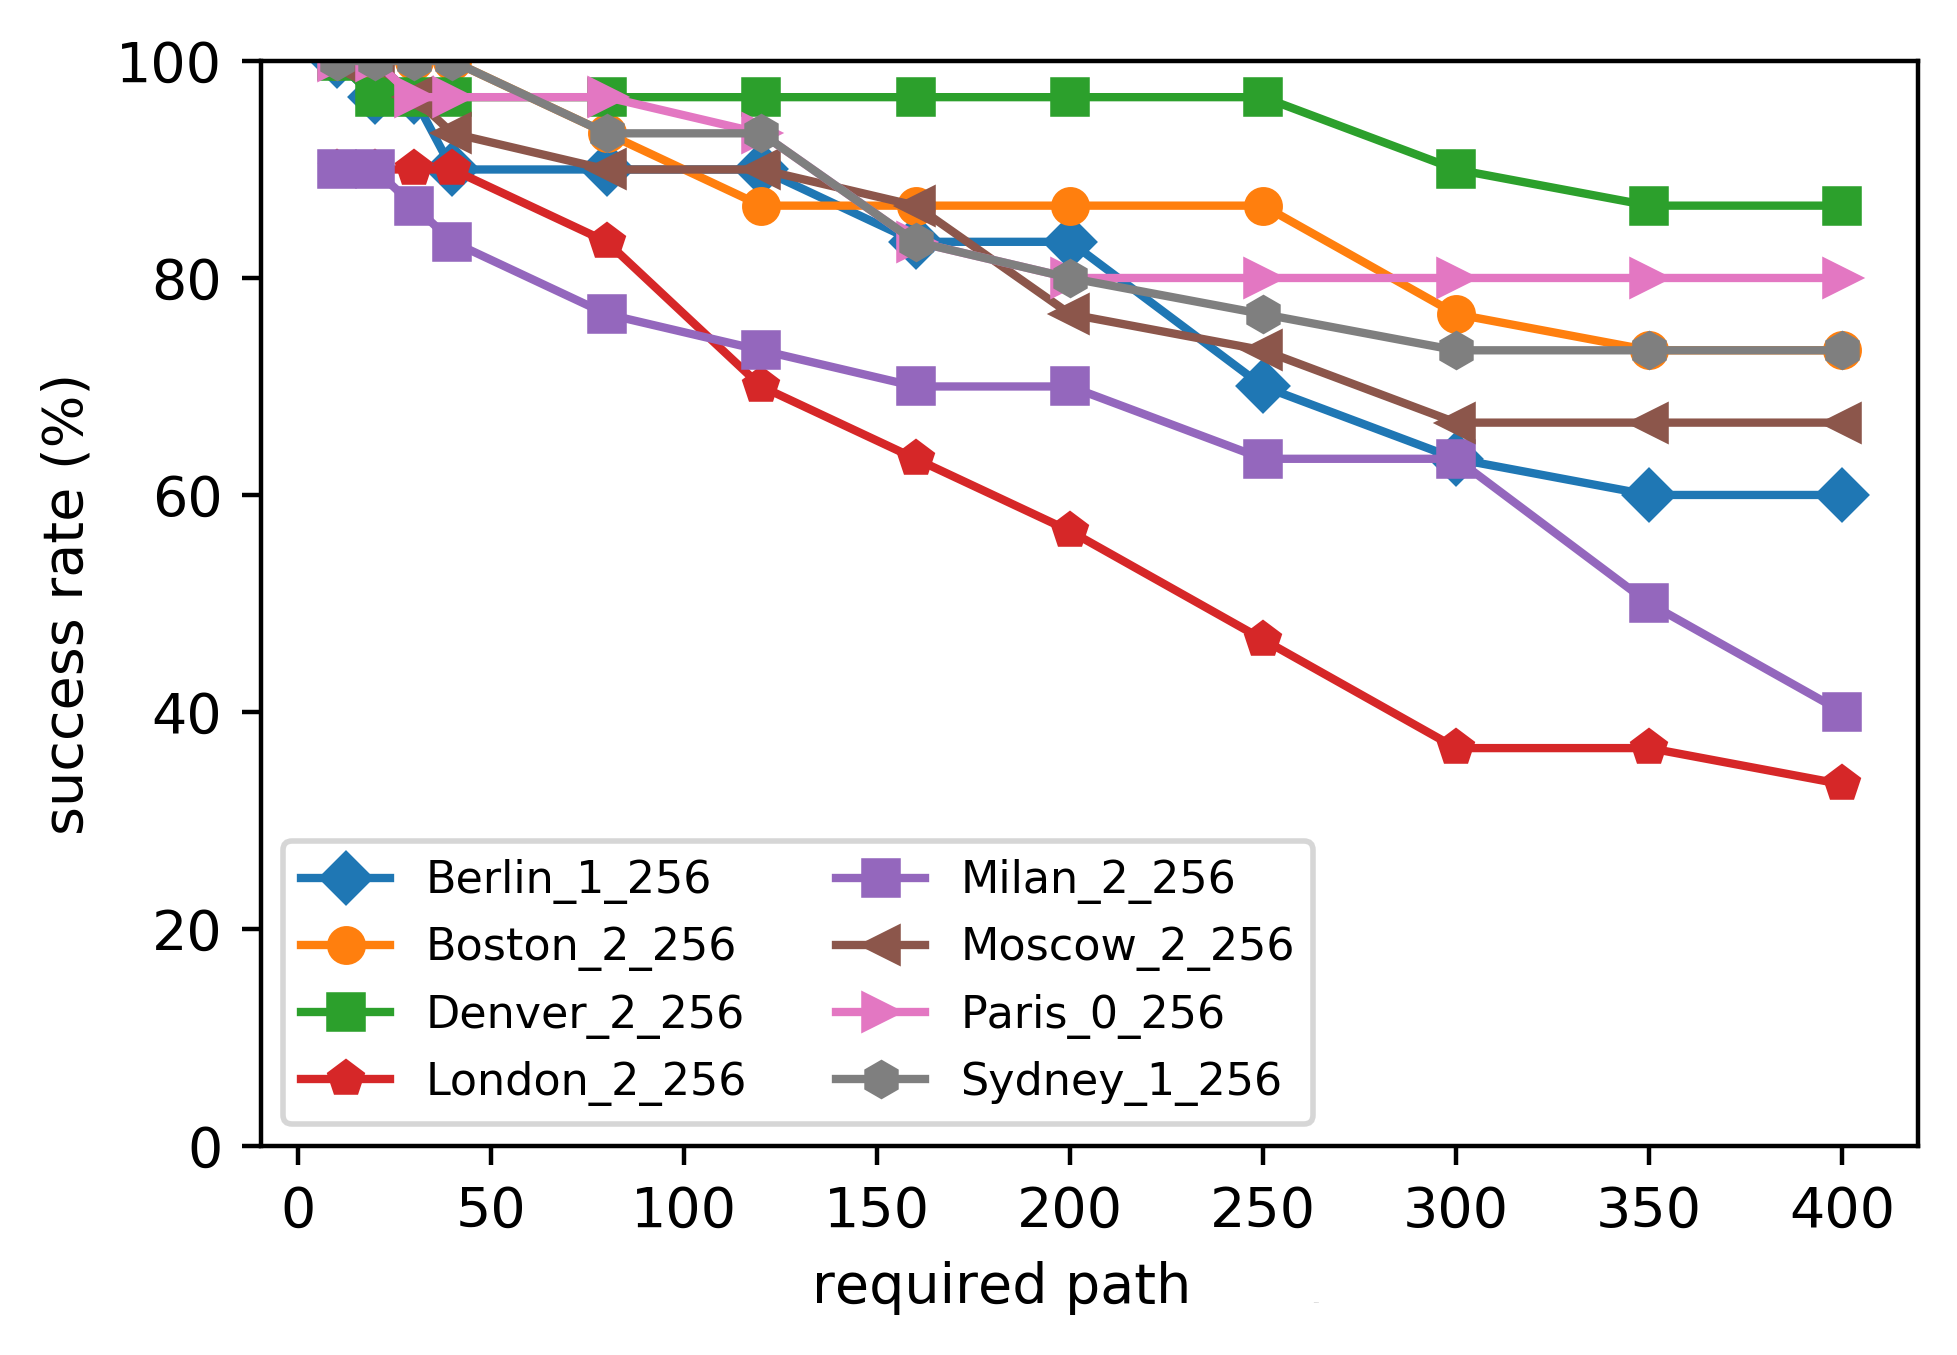
\includegraphics[width=4.6cm]{RHCF_succ_and_count.png}}
  \centerline{C: RHCF}
\end{minipage}
\hfill
\begin{minipage}{.245\linewidth}
  \centerline{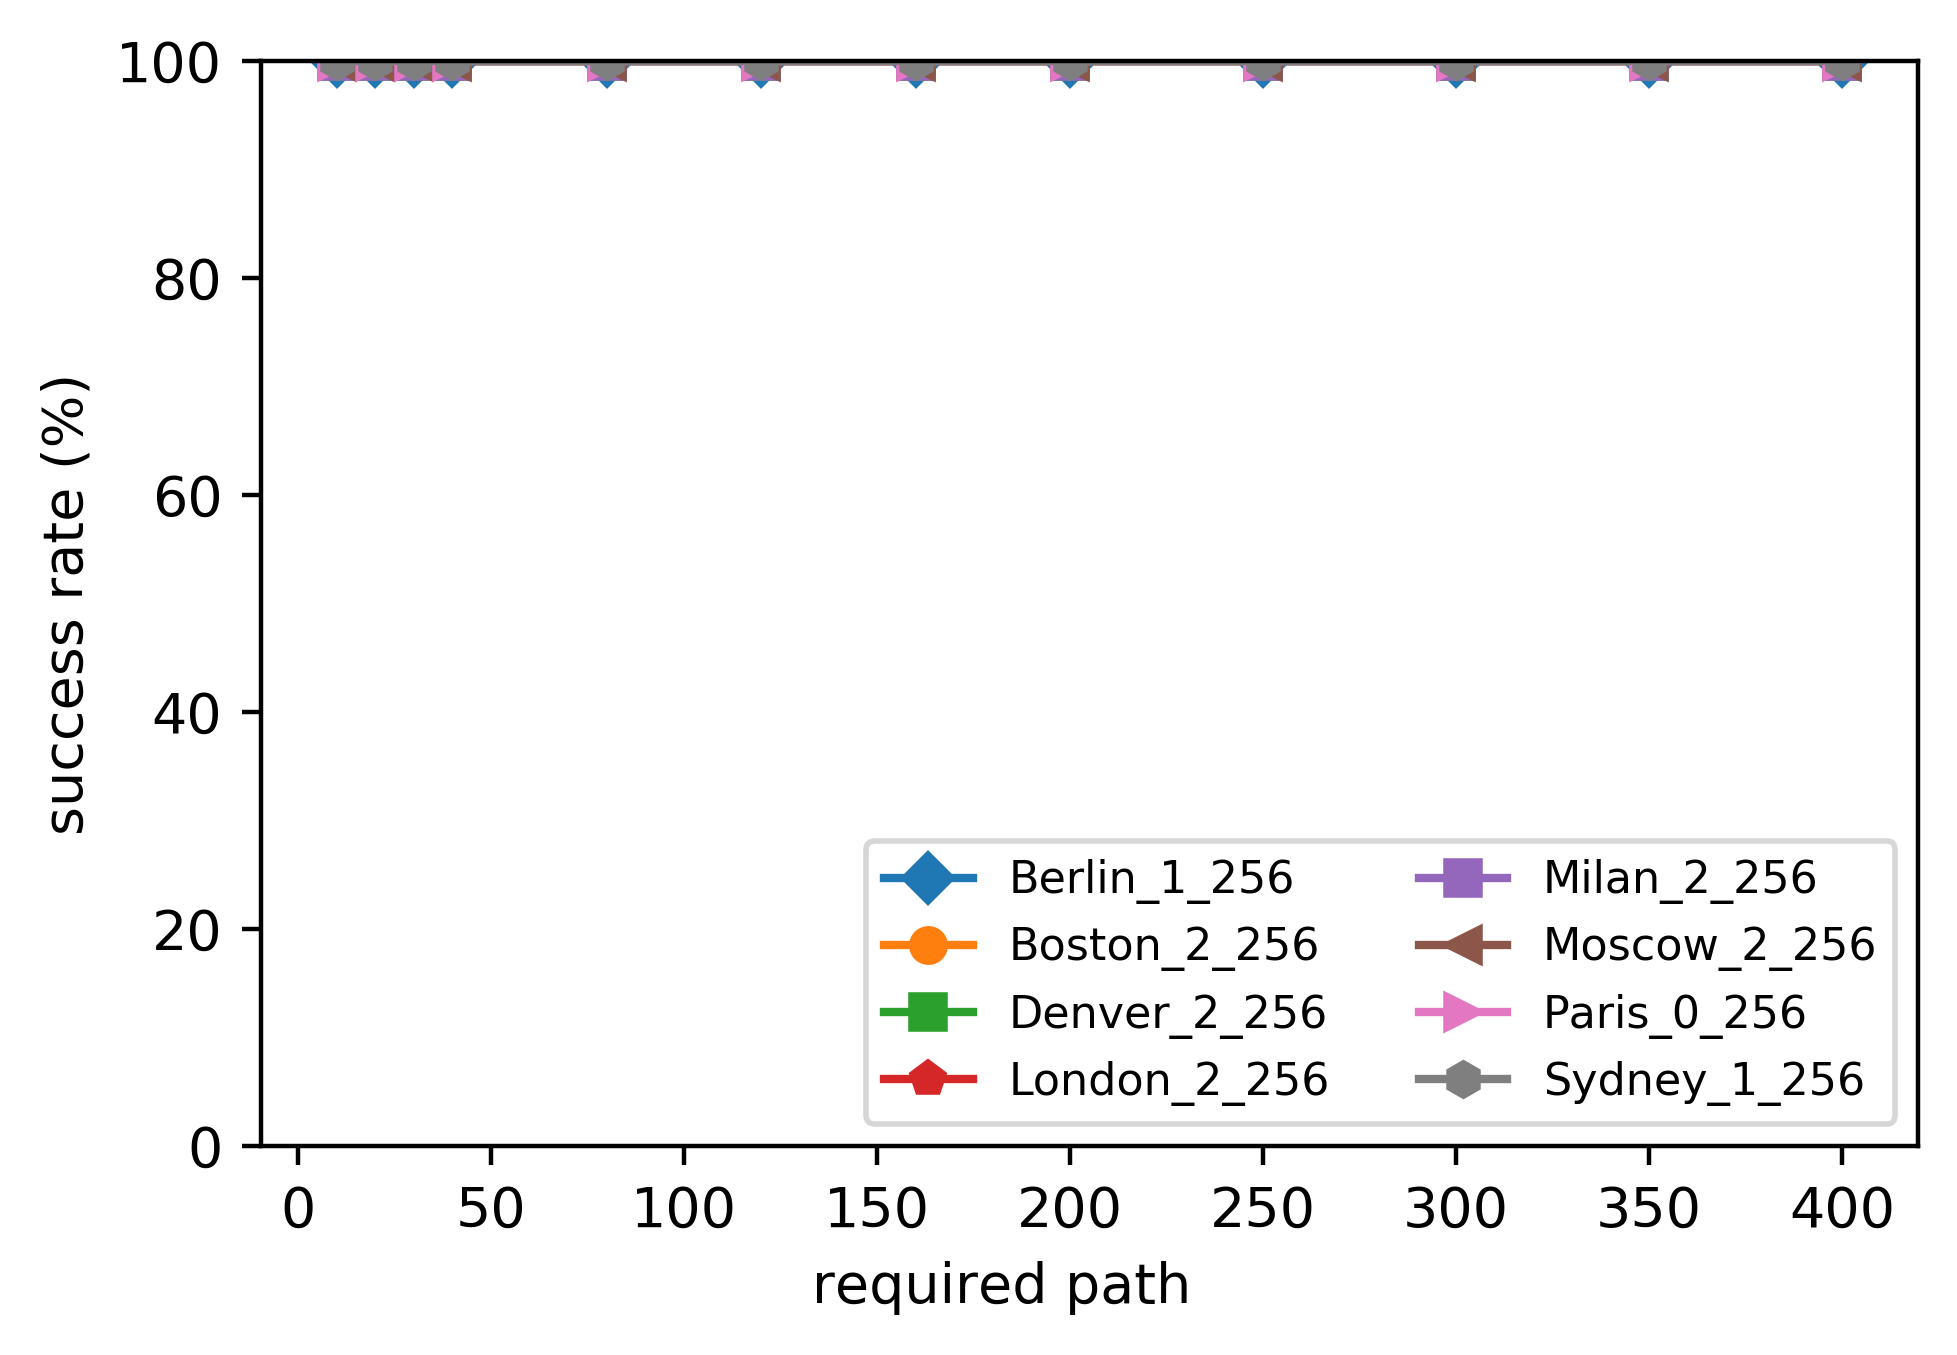
\includegraphics[width=4.6cm]{RJ_succ_and_count.png}}
  \centerline{D: Our method}
\end{minipage}
\vfill

\caption{These figures illustrate the mean success rate for finding the required number of paths for each map using all four methods. The magnification for all maps is set to 1.0. 
}
\label{succ_and_path_count}
\end{figure*}

\begin{figure}[t] \scriptsize
%\begin{tabular}{cc}
\begin{minipage}{.48\linewidth}
  \centerline{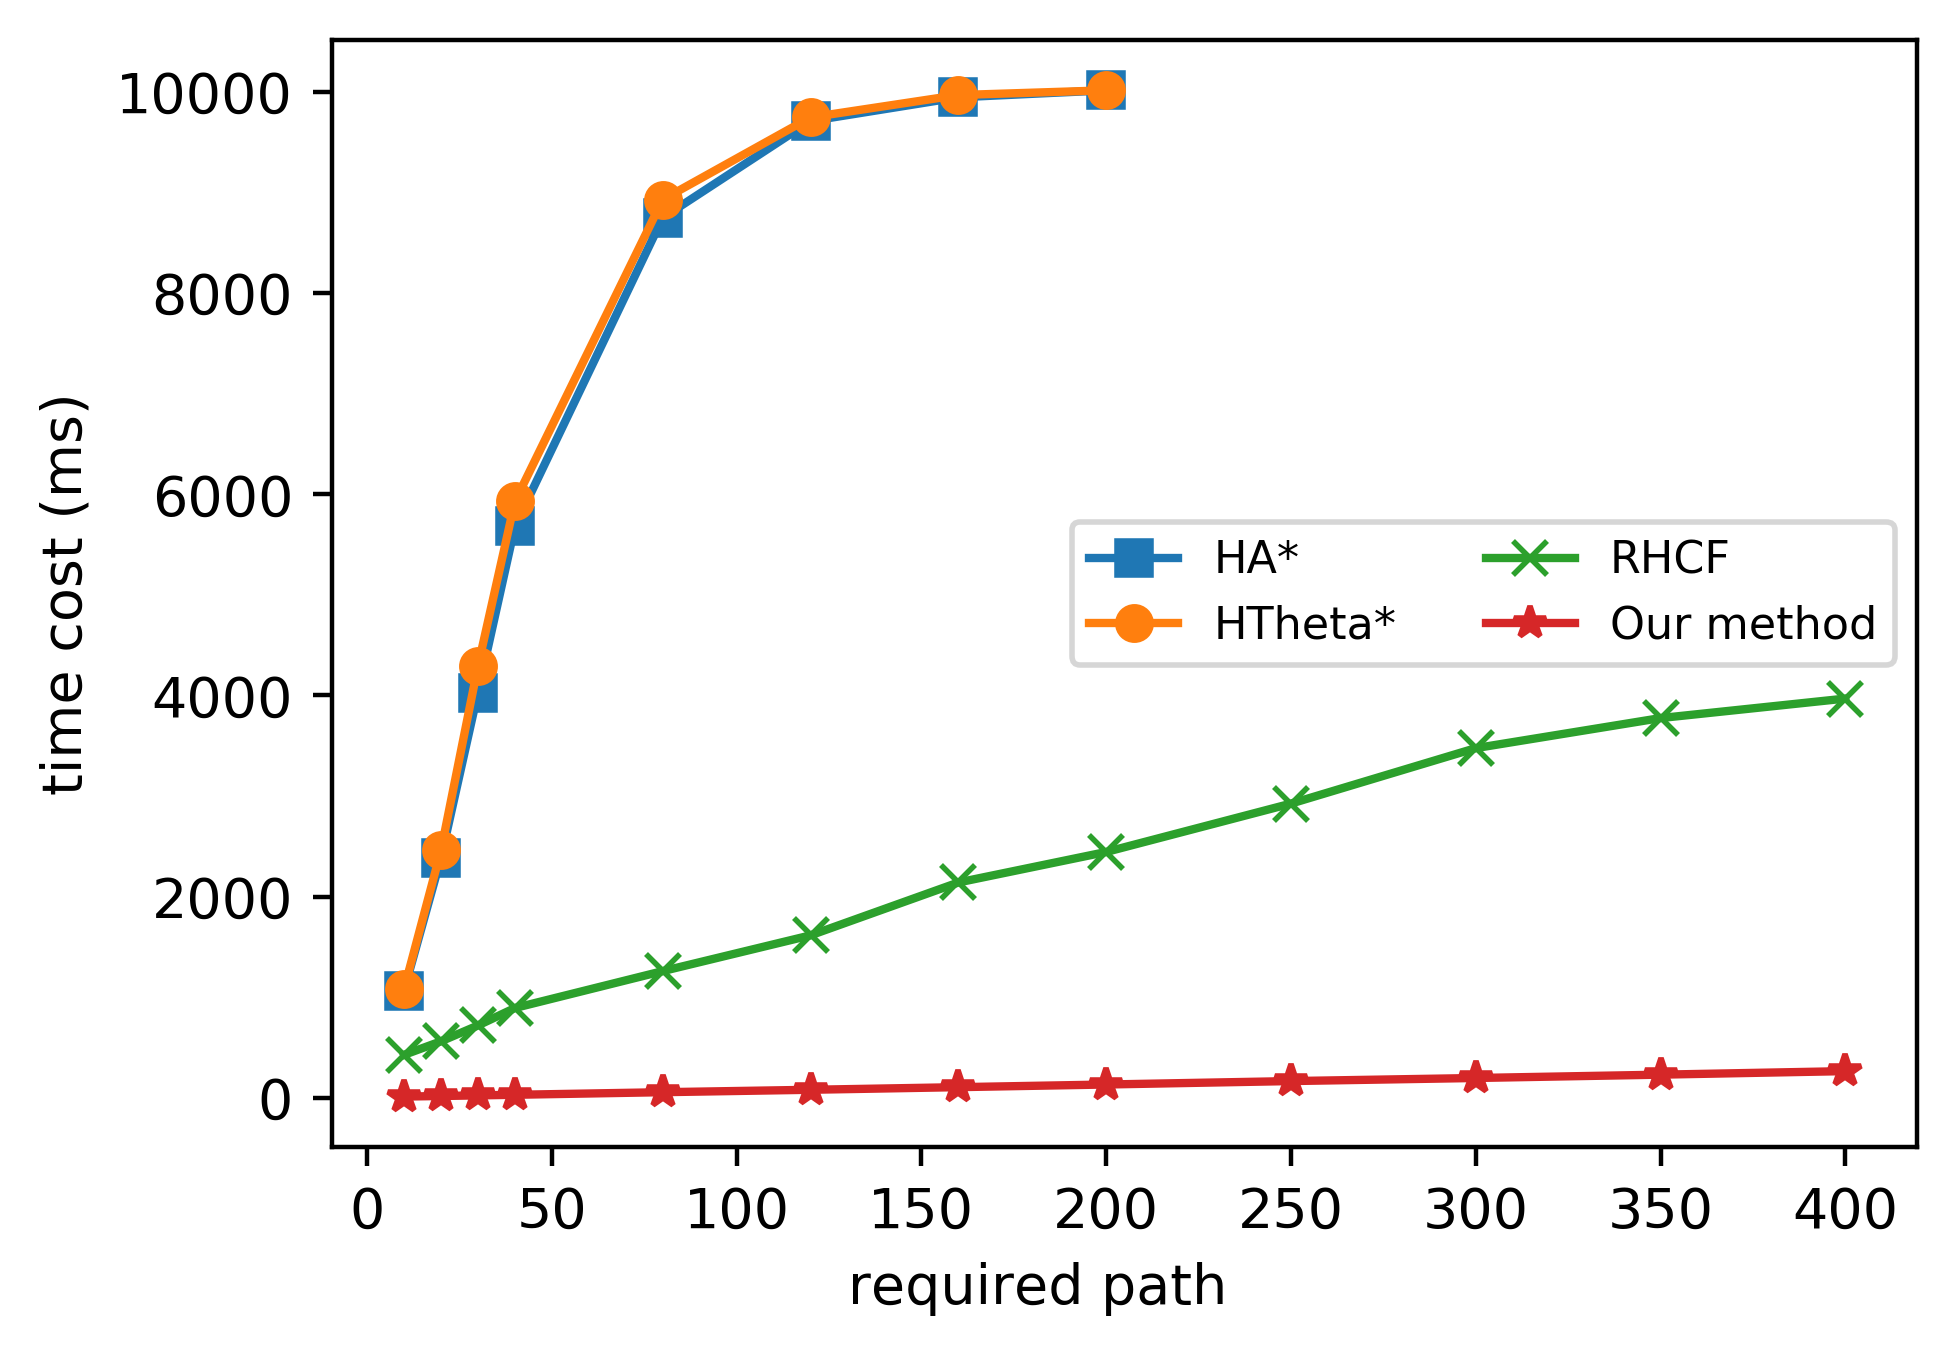
\includegraphics[width=4.6cm]{comparison_time_and_count.png}}
  \centerline{A: time cost comparison}
\end{minipage}
\hfill
\begin{minipage}{.48\linewidth}
  \centerline{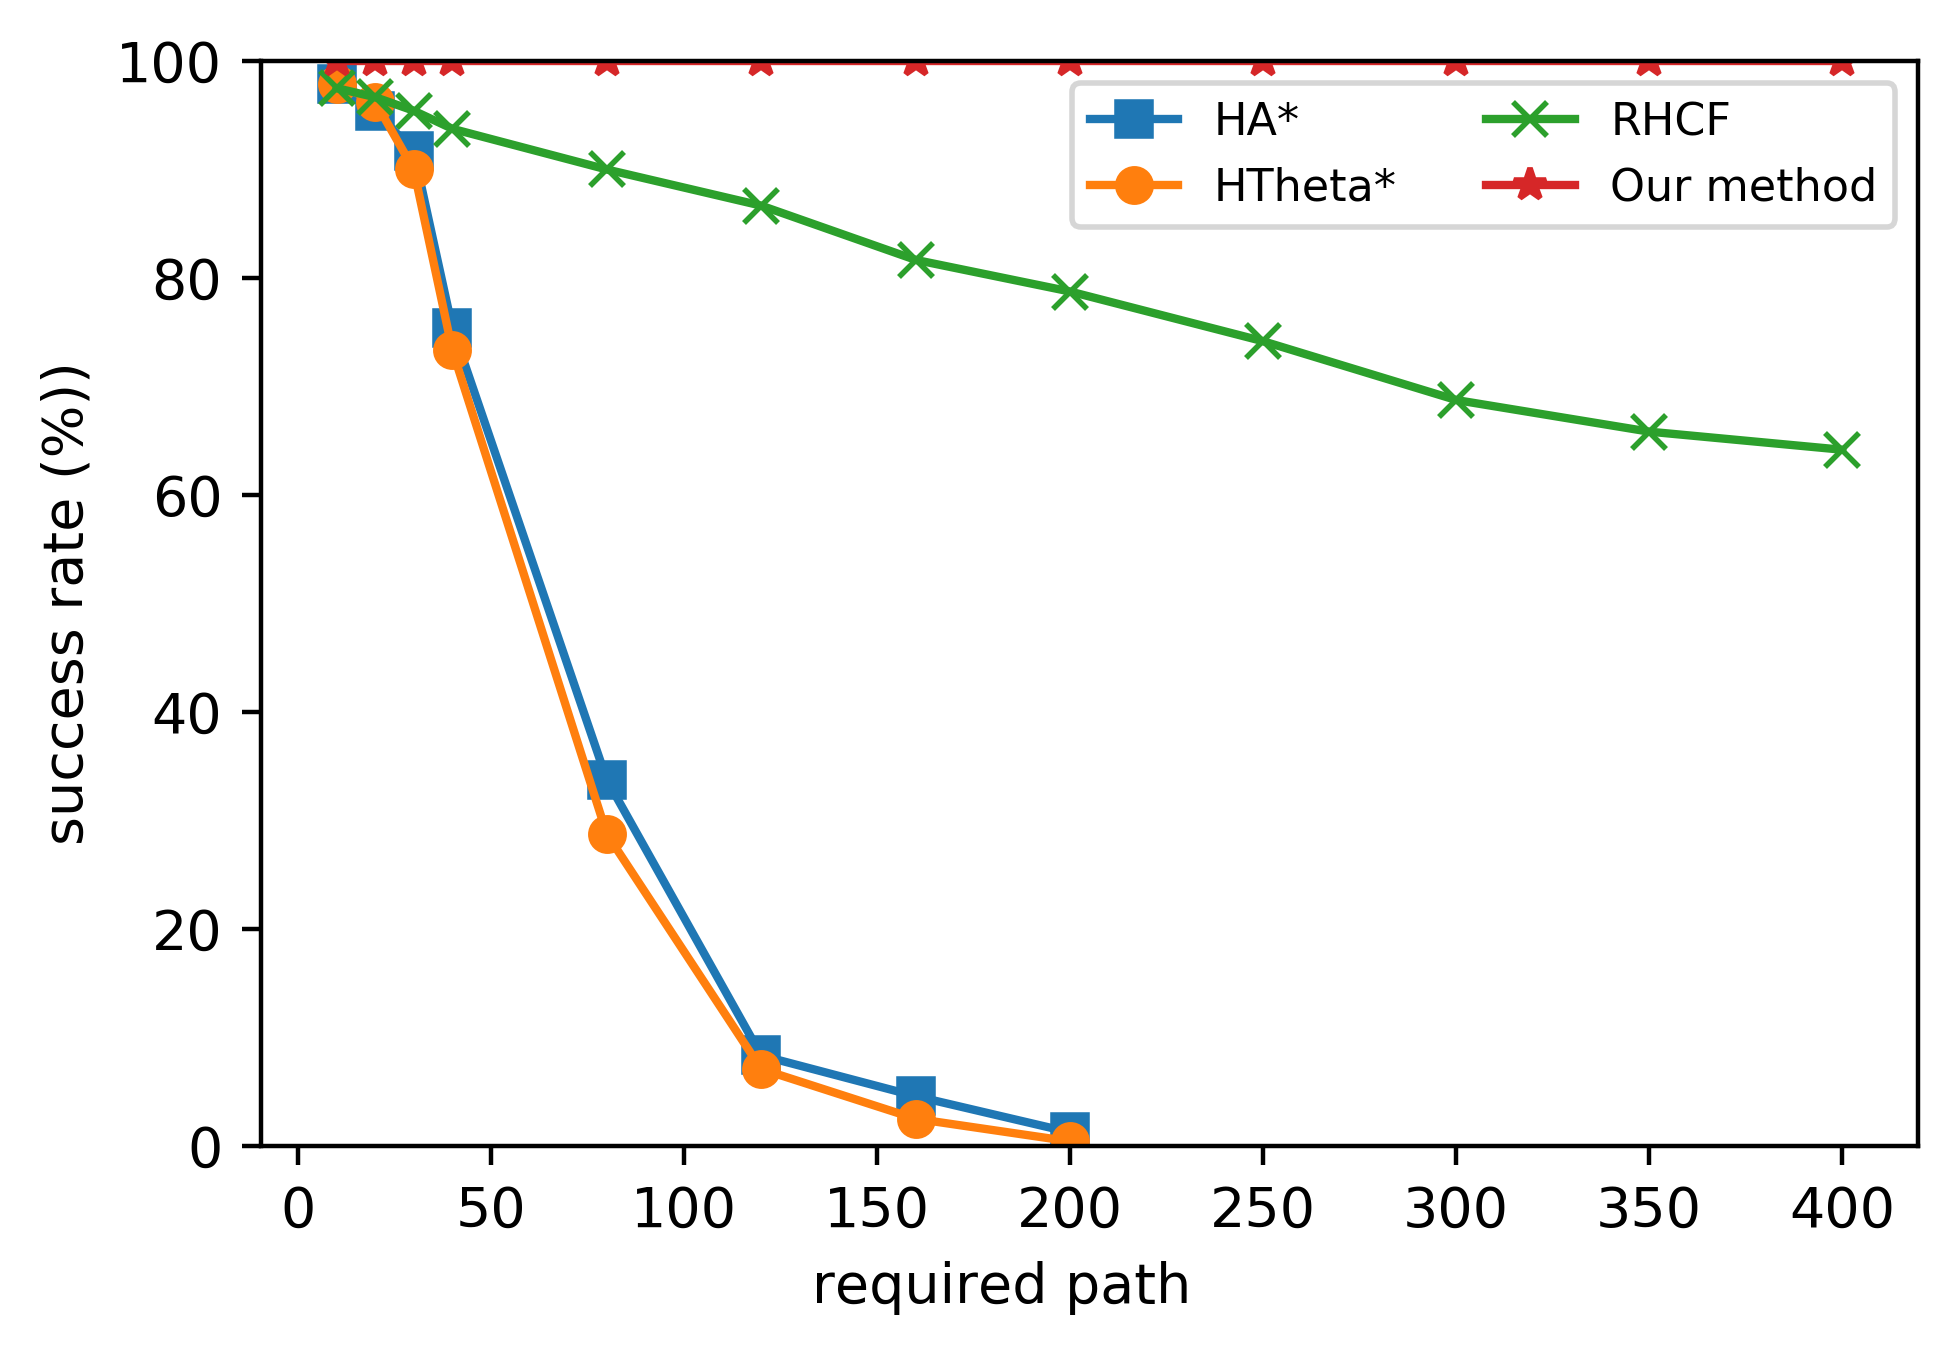
\includegraphics[width=4.6cm]{comparison_succ_and_count.png}}
  \centerline{B: success rate comparison}
\end{minipage}
\vfill

\caption{These figures show the comparison of the success rates and time costs of the four methods across all eight maps, with a consistent magnification set to 1.0.}
\label{compariosn_between_methods}
\end{figure}


%Firstly, we test all four methods under the mentioned eight maps, use them to find multiple (range from 10 to 400) topologically distinctive paths, and we recorded the mean time cost and success rate under each maps, as shown in Fig. \ref{total_time_cost_and_path_count} and Fig. \ref{succ_and_path_count} respectively. The combined results of time cost and success rate are shown in Fig. \ref{compariosn_between_methods}.

%As shown in Fig. \ref{total_time_cost_and_path_count} and Fig. \ref{succ_and_path_count}, our method's mean time cost to find 400 paths is 500ms approximately, and its success rate is 100\%. While for RHCF, it take approximately 7s to find 400 paths in average under the worst case and its success rate is decrease to 80\% in the best case and 40\% in the worst case. For HA* and HTheta*, their mean time cost is close to the time upper bound (10s) when try to find more than 80 paths. And their success rate decreases as mean time cost increases, it decreases to 50\% after try to find more than 40 paths.   And our method's time cost increase in a slower way than other methods, as our method avoid mutiple graph search for multiple path but get all required paths during one times of search. Out method only take 500ms in average in the worst case, and always are 100\% to find required number of paths.

%In this section, our method demostrate overwhelming advantage to other methods in term of time cost and success rate. 

Initially, we subjected all four methods to testing under the specified eight maps, utilizing them to search varying numbers of topologically distinctive paths (ranging from 10 to 400). The mean time cost and success rate were recorded for each map, as depicted in Fig. \ref{total_time_cost_and_path_count} and Fig. \ref{succ_and_path_count} respectively. The amalgamated results, showcasing the interplay between time cost and success rate, are illustrated in Fig. \ref{compariosn_between_methods}.

As illustrated in Fig. \ref{total_time_cost_and_path_count} and Fig. \ref{succ_and_path_count}, our method achieves a mean time cost of approximately 500ms to find 400 paths, boasting a 100\% success rate. In contrast, RHCF takes around 7s to find 400 paths on average, with its success rate varying from 80\% in the best case to 40\% in the worst case. For HA* and HTheta*, their mean time cost approaches the time upper bound (10s) when attempting to find more than 80 paths. Moreover, their success rate declines as the mean time cost increases, dropping to 50\% after attempting to find more than 40 paths. Notably, our method exhibits a slower increase in time cost compared to other methods, as it circumvents multiple graph searches for multiple paths, obtaining all required paths in a single search. With an average time cost of only 500ms in the worst case, our method consistently achieves a 100\% success rate in finding the required number of paths.

This section underscores our method's substantial advantage over other methods in terms of time cost and success rate.

\subsubsection{Path length}

% time and scale
\begin{figure*}[t] \scriptsize
%\begin{tabular}{cc}
\begin{minipage}{.245\linewidth}
  \centerline{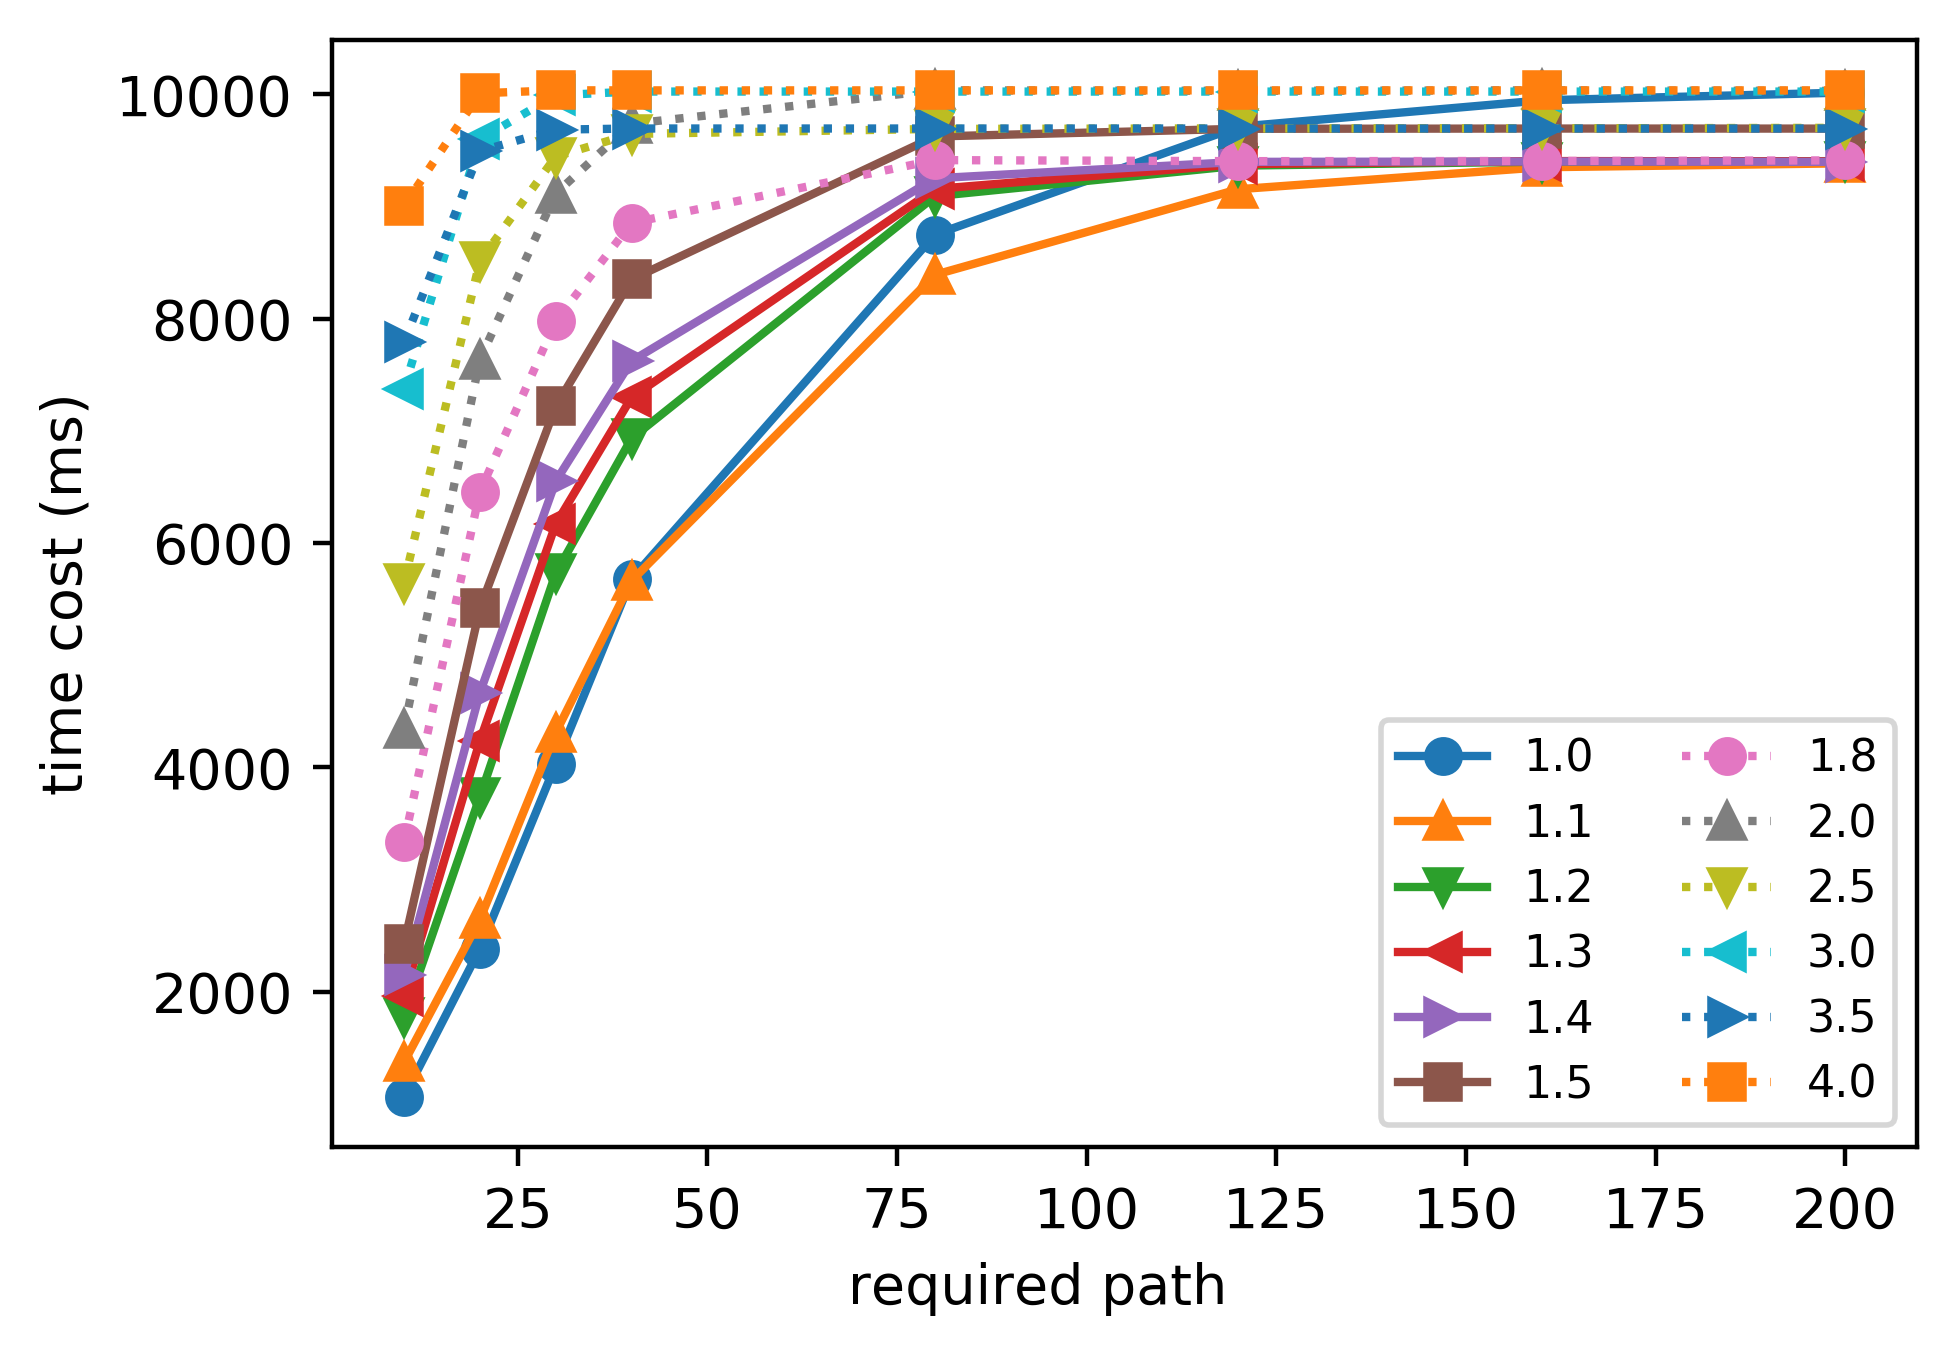
\includegraphics[width=4.6cm]{HsAs_scale_cost_method_path_count.png}}
  \centerline{A: HA*}
\end{minipage}
\hfill
\begin{minipage}{.245\linewidth}
  \centerline{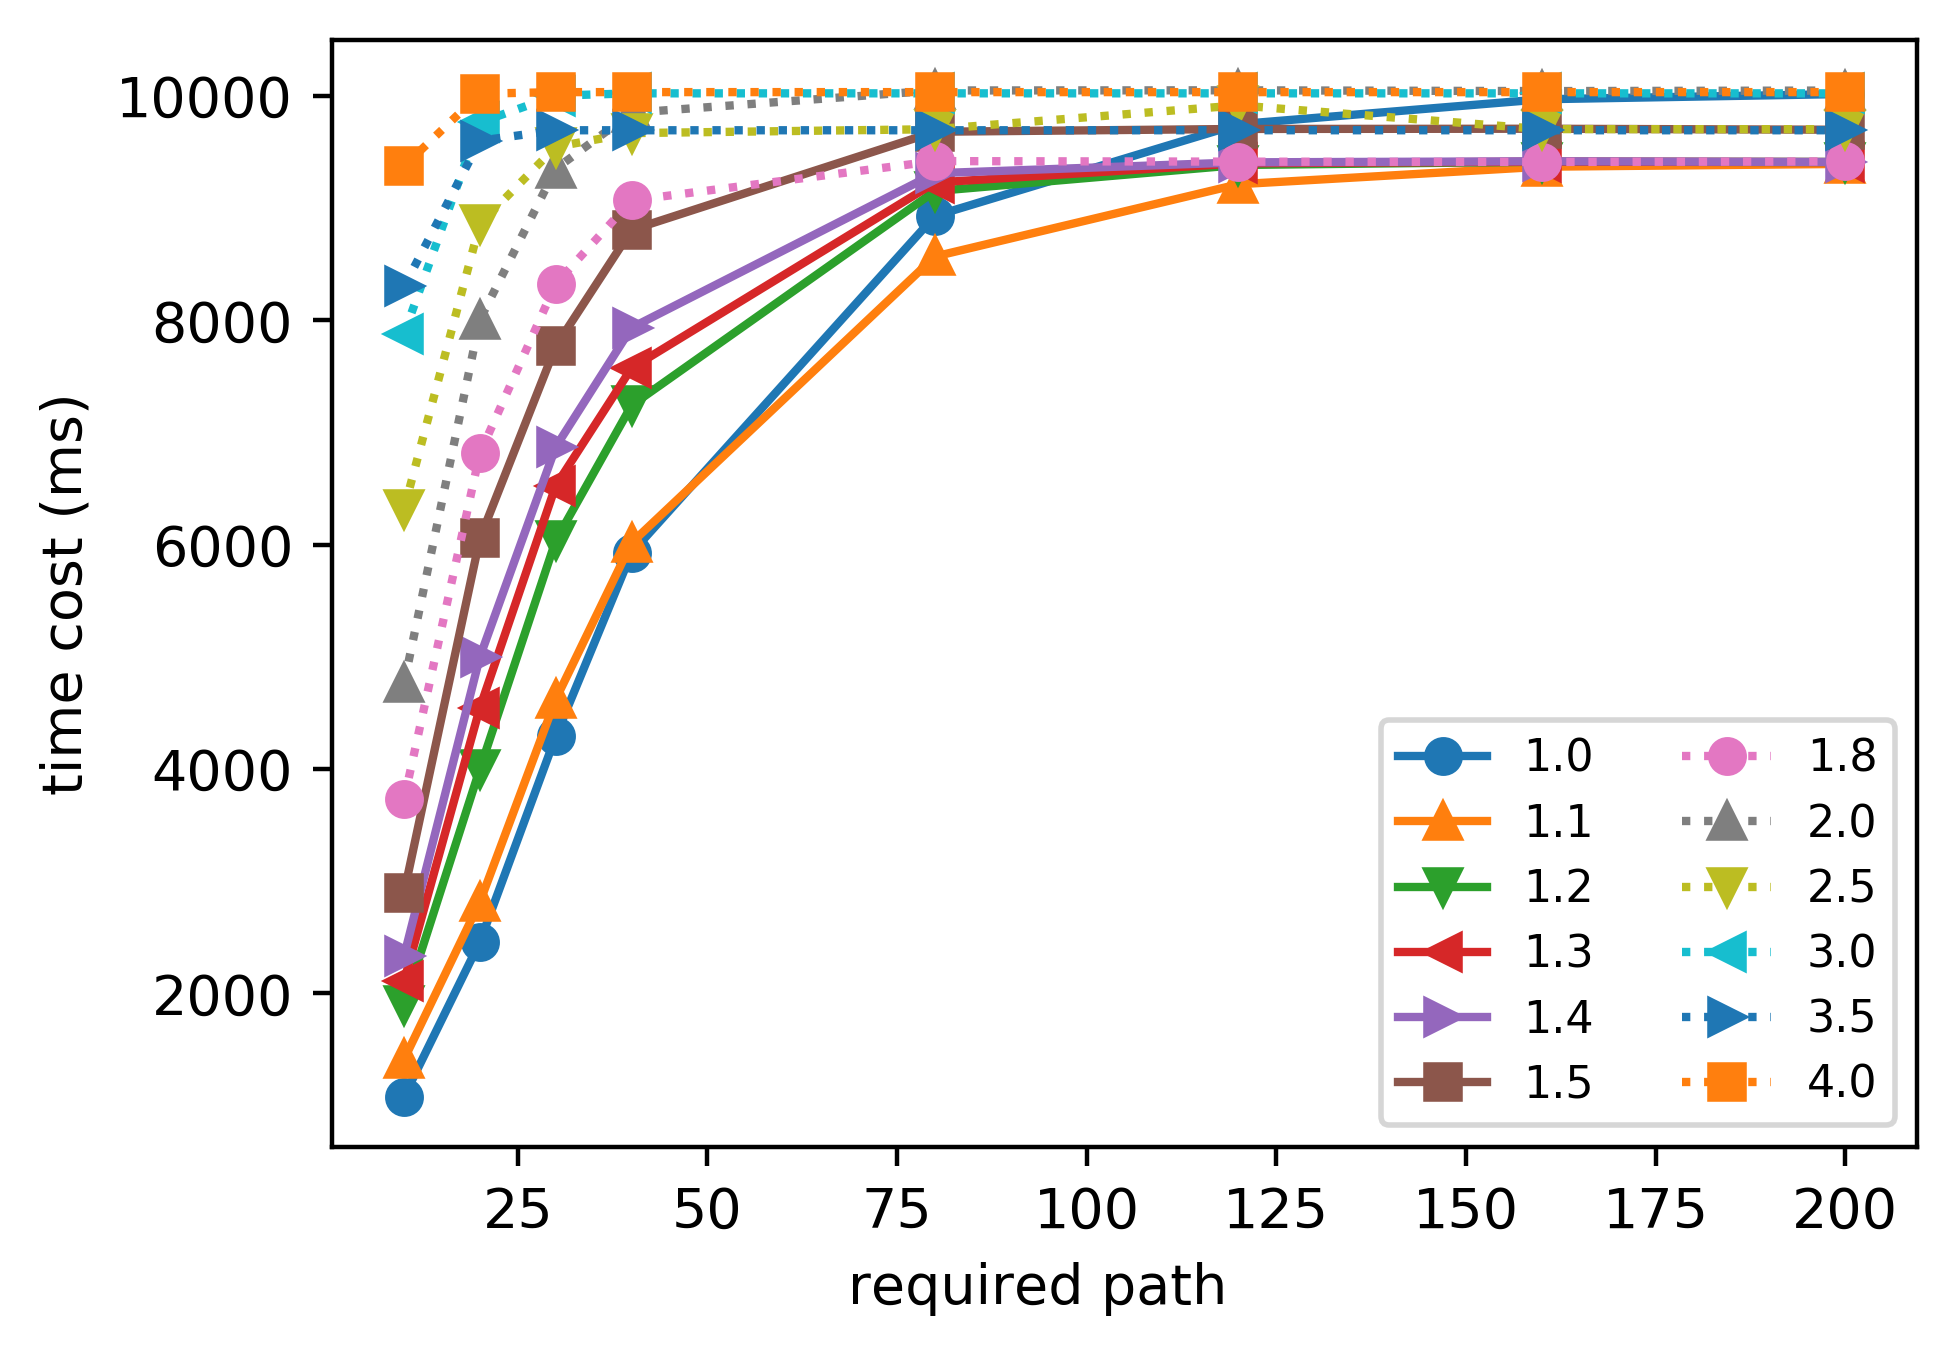
\includegraphics[width=4.6cm]{HsTs_scale_cost_method_path_count.png}}
  \centerline{B: HTheta*}
\end{minipage}
\hfill
\begin{minipage}{.245\linewidth}
  \centerline{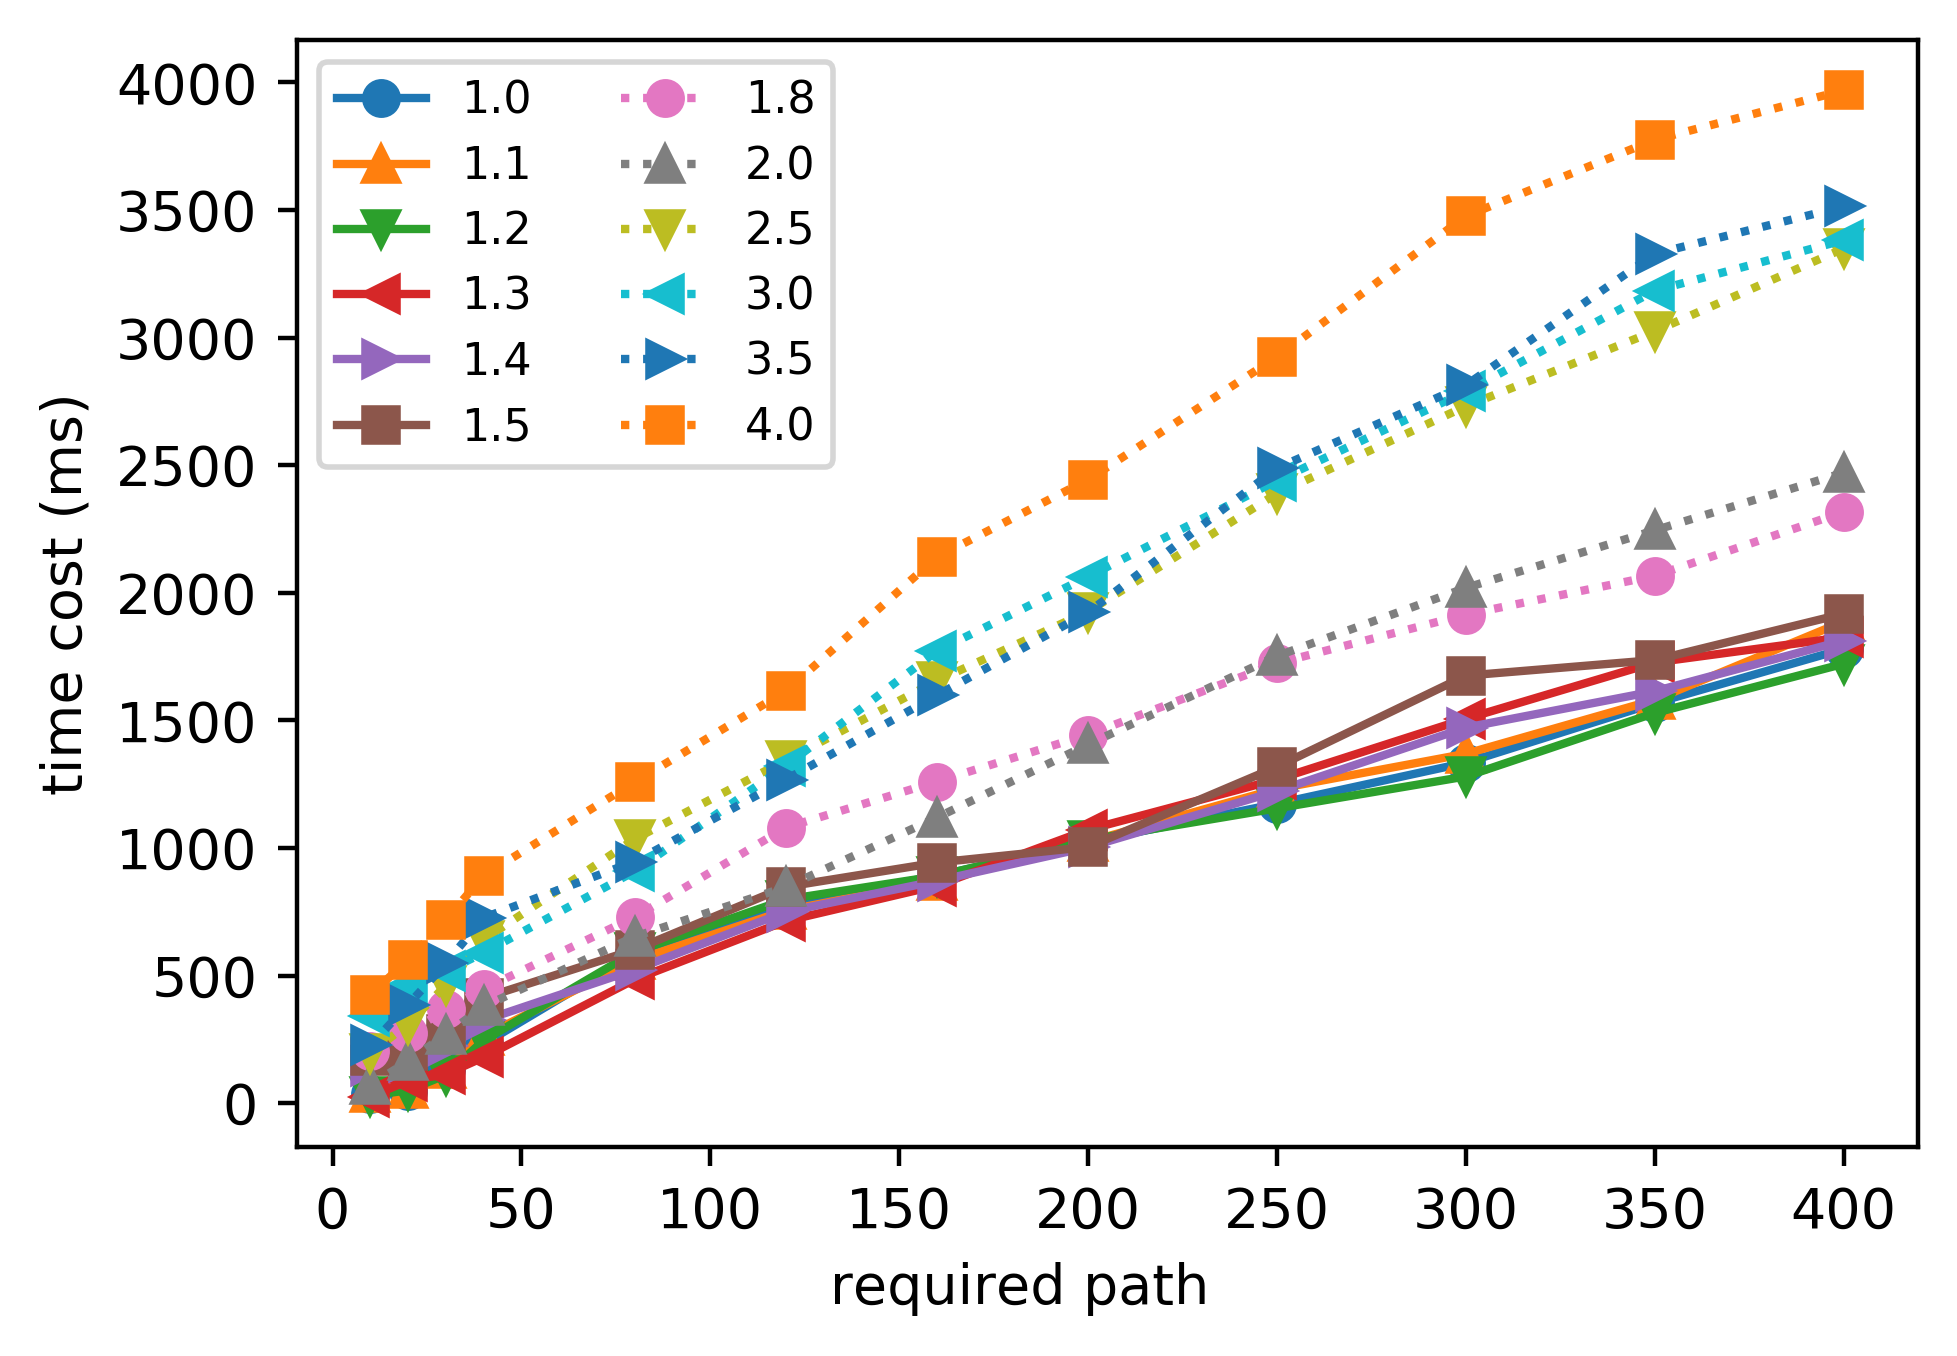
\includegraphics[width=4.6cm]{RHCF_scale_cost_method_path_count.png}}
  \centerline{C: RHCF}
\end{minipage}
\hfill
\begin{minipage}{.245\linewidth}
  \centerline{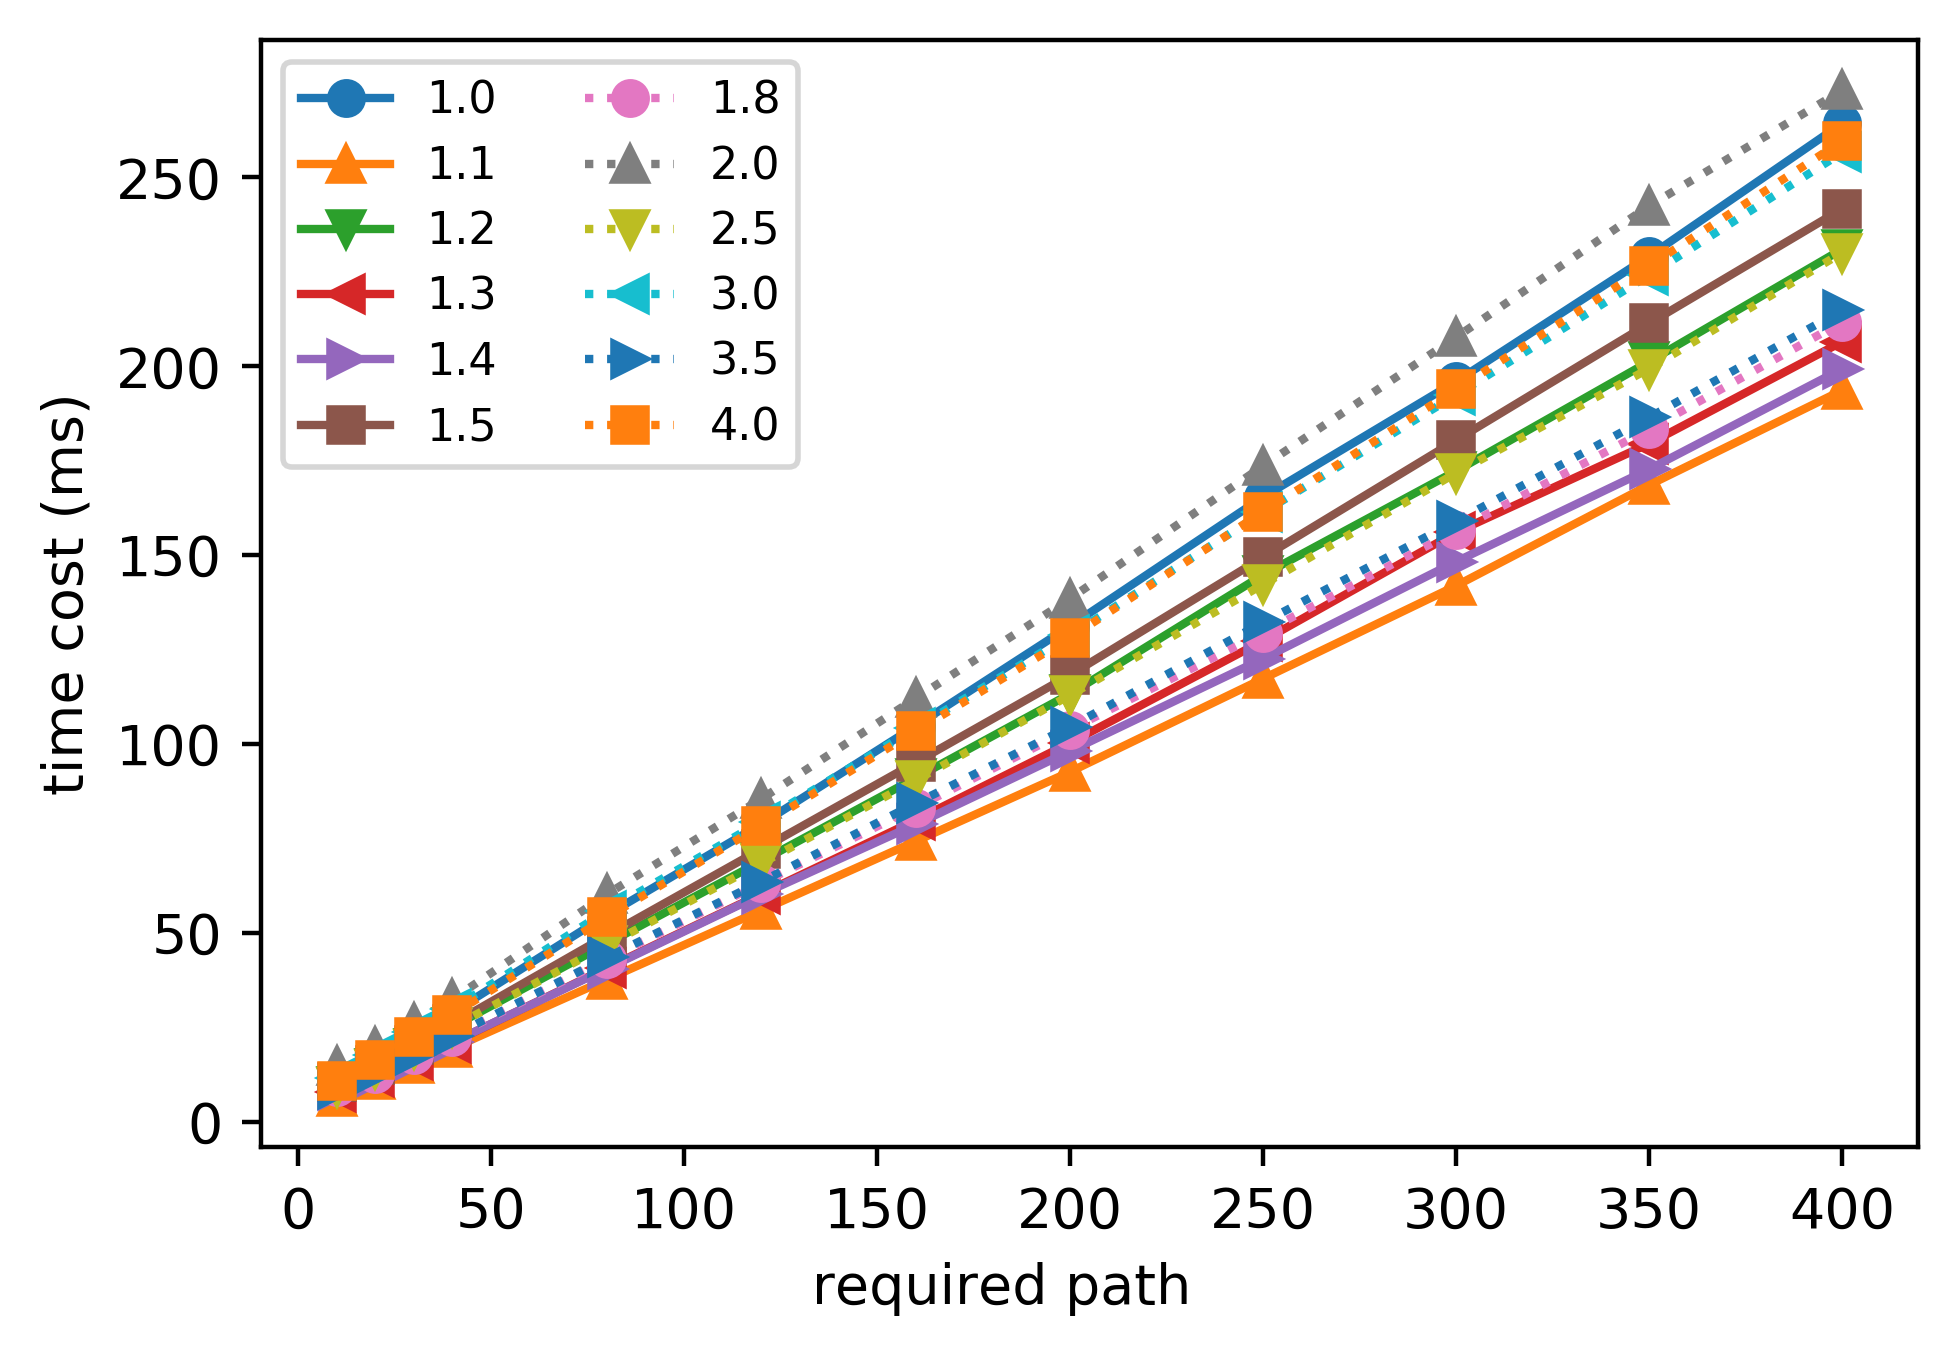
\includegraphics[width=4.6cm]{RJ_scale_cost_method_path_count.png}}
  \centerline{D: Our method}
\end{minipage}
\vfill

\caption{These figures illustrate that the mean time cost to find the required number of paths increases with the magnification of the maps, covering all eight maps.}
\label{scale_cost_method_path_count}
\end{figure*}

% success rate and scale
\begin{figure*}[t] \scriptsize
%\begin{tabular}{cc}
\begin{minipage}{.245\linewidth}
  \centerline{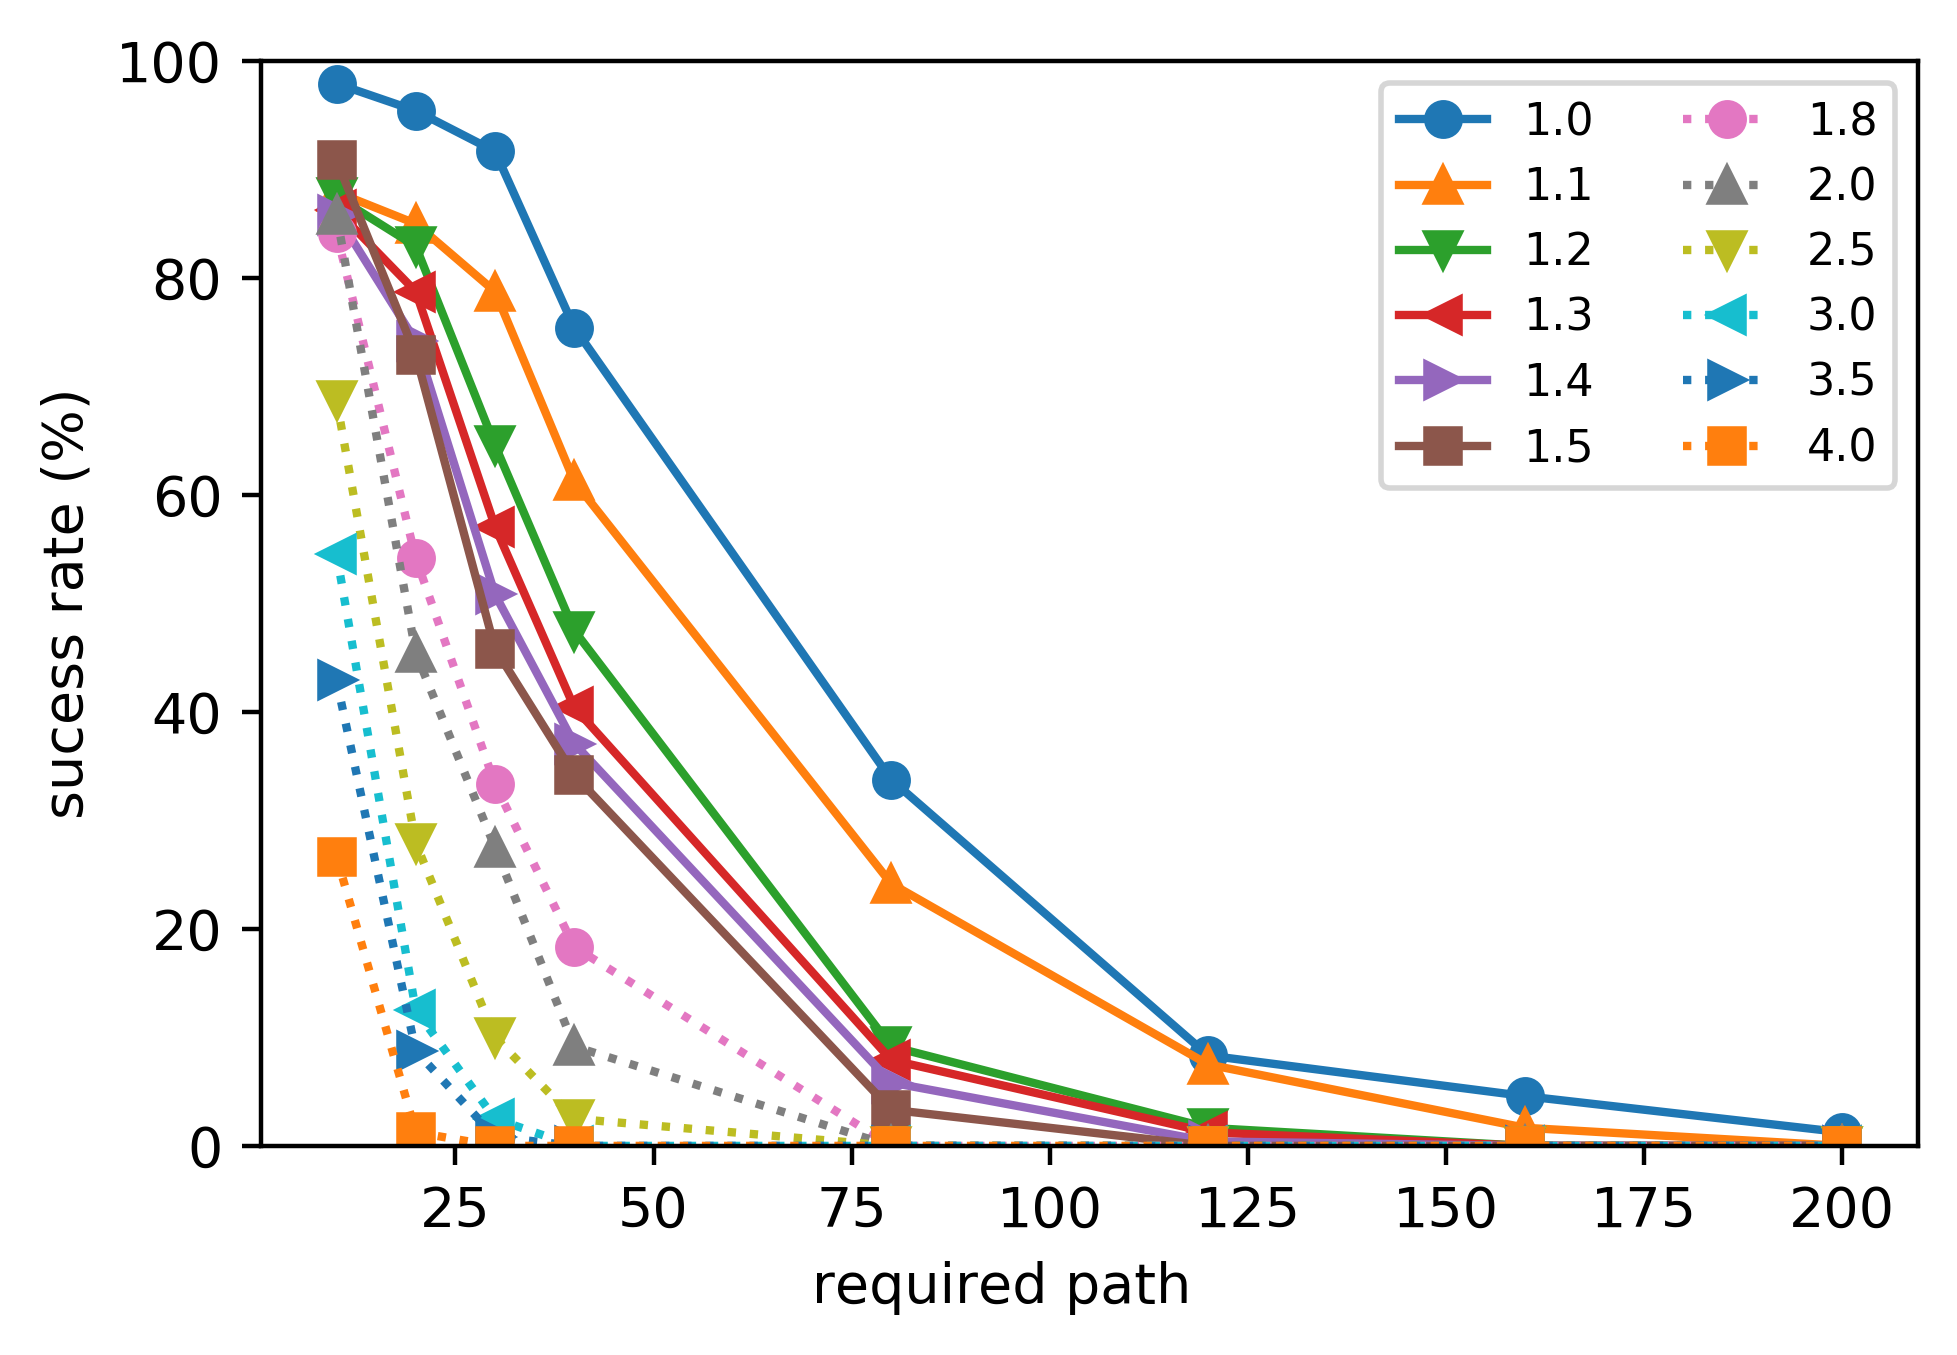
\includegraphics[width=4.6cm]{HsAs_scale_succ_method_path_count.png}}
  \centerline{A: HA*}
\end{minipage}
\hfill
\begin{minipage}{.245\linewidth}
  \centerline{\includegraphics[width=4.6cm]{HsTs_scale_succ_method_path_count.png}}
  \centerline{B: HTheta*}
\end{minipage}
\hfill
\begin{minipage}{.245\linewidth}
  \centerline{\includegraphics[width=4.6cm]{RHCF_scale_succ_method_path_count.png}}
  \centerline{C: RHCF}
\end{minipage}
\hfill
\begin{minipage}{.245\linewidth}
  \centerline{\includegraphics[width=4.6cm]{RJ_scale_succ_method_path_count.png}}
  \centerline{D: Our method}
\end{minipage}
\vfill

\caption{These figures illustrate that the mean success rate to find the required number of paths increases with the magnification of the maps, covering all eight maps.}
\label{scale_succ_method_path_count}
\end{figure*}

\begin{figure}[t] \scriptsize
%\begin{tabular}{cc}
  \centerline{\includegraphics[width=4.6cm]{method_path_length.png}}
  \centerline{mean path length comparison}
\caption{These figures present a comparison of path lengths among the four methods when the required number of paths is set to 10. The results from all maps are combined, with a consistent magnification of 1.0 for all maps. }
\label{compariosn_path_length}
\end{figure}


%Path length is also a crucial attribute of path planning, so we compare path length of all four methods in this section. However, we notice than for methods that cost more time for longer paths, such as HA* and HTheta*, they find only short path and failed to find the required number of paths. So it is unfair to compare mean path length under all required path count, as HA* and HTheta* find only short path while RHCF and our method as capable to find more and longer path. So in this section, we only compare path length when find 10 topologically distinctive paths, which all method's success rate is more than 90\%,  as shown in Fig. \ref{compariosn_path_length}. It is obvious that RHCF has the longest path, as its based on Voronoi Graph . Both HTheta* and HA* have shorter path than RHCF, as they are A* based shortest path finding. But HTheta* and our method have shorter path than HA*, as both tangent graph based path planning and HTheta* are any angle shortest path planning, while A* uses four-neighbor or eight-neighbor expansion.

Path length, a critical attribute in path planning, is the focus of comparison among all four methods in this section. However, it's worth noting that methods like HA* and HTheta*, which incur longer computation times for extended paths, may prioritize finding shorter paths and consequently may not reach the required number of paths. To ensure fairness in our comparison, we exclusively examine path lengths when finding 10 topologically distinctive paths, a scenario where all methods achieve a success rate exceeding 90\%, as depicted in Fig. \ref{compariosn_path_length}.

Notably, RHCF exhibits the longest paths, given its reliance on the Voronoi Graph. Both HTheta* and HA* yield shorter paths than RHCF, as they are rooted in A*-based shortest path finding. Interestingly, HTheta* and our method achieve shorter paths than HA*, leveraging tangent graph-based path planning and the any-angle shortest path planning characteristic of HTheta*, whereas A* relies on four-neighbor or eight-neighbor expansion.
     
\subsubsection{Map scale and time cost}

In this section, our focus centers on exploring the relationship between mean time cost and map scale. We conducted tests for all four methods across eight maps with varying magnifications, recording the mean time cost and success rate for different required numbers of paths, as depicted in Fig. \ref{scale_cost_method_path_count} and Fig. \ref{scale_succ_method_path_count}.

As evident in these figures, HA* and HTheta*'s time cost increases significantly, and their success rate decreases as the map magnification scales from 1.0 to 4.0. This decrease is more pronounced as the larger map size requires more node expansions and H-signature calculations.

RHCF exhibits a similar trend, although in a milder manner. The size of the Voronoi graph remains relatively unchanged, but determining connections from start/target to the graph takes more time with larger maps.

In contrast, our method demonstrates a gradual increase in time cost. The main factors influencing its cost are the number of required paths and the size of the tangent graph, which remains almost constant with increasing map scale. The slight fluctuations in our method's cost are attributed to the minor volatility in the CPU's computational performance.

In conclusion, our method demonstrates stability with increasing map scale. It incurs a gradual increase in time cost while maintaining a 100\% success rate, contrasting sharply with the notable decline in performance observed in other methods. The resilience of our method as map scale increases can be ascribed to the consistent behavior of the tangent graph, which remains stable in both size and time cost of construction, responding adeptly to variations in scale.

\section{Discussion and conclusion}
\label{Conclusion}

In this article, we introduce a tangent graph-based topologically distinctive path planning algorithm. It leverages the property that tangents form locally shortest paths, and any two locally shortest paths belong to different topologies. Compared to existing algorithms, our approach requires no indicator to determine whether two paths belong to the same topology. Furthermore, it eliminates the need to repeat the search for multiple paths, as all distinctive paths can be found in a single search.

To address the challenge of the exponential growth in queue size during breadth-first search, we propose an expansion reduction technique. This approach significantly reduces the time cost of searching for multiple paths while preserving computational complexity.

Our method consists of two main steps: the construction of the tangent graph and the search for multiple paths. We employ the ENL-SVG technique, as introduced by \cite{oh2017edge}, to construct the tangent graph, leveraging the advantages offered by line-of-sight scans. Additionally, to avoid repeating these calculations every time the map is loaded, we save the results to a binary file, which is then loaded during the framework loading process, saving valuable time.

During the search for multiple paths, we introduce loop avoidance to prevent the repetition of waypoints in the path and avoid intersections with itself. Additionally, we apply the taut condition of \cite{oh2017edge} to ensure every path is locally shortest. It's important to note that as the number of waypoints in the path increases, the time cost of loop detection also increases. Experimental results show that the ratio of no-loop constraint checks in the total cost increases as the required number of paths increases. This occurs because the requirement for more paths often results in paths with a larger number of waypoints.

In comparison with other methods, our approach demonstrates significant efficiency when compared to RHCF, HA*, and HTheta*. Specifically, our method takes approximately 250ms to determine 400 paths from the mentioned public map dataset, while RHCF takes more than 1 second, and HA* and HTheta* take more than 10 seconds. And our method's performance is stable as the scale of map increases. However, it's important to note that our method has a limitation in that it cannot search for multiple paths with the same topology, unlike methods that use indicators like H-signature, which are capable of searching for multiple paths with the same topology. And the current version of our method is not suited for 3D Euclidean space, which limit its application.

In the future, we plan to research how to apply our method to 3D maps and implement our method using multiple threads, as currently, it operates in a single thread. Since there is no dependence between different unfinish paths during the search process, there will be no loss of complexity when utilizing multiple threads. Additionally, we intend to apply our method to trajectory optimizations. Given that our method can provide hundreds of topologically distinctive paths in real time, it is crucial to study how to speed up trajectory optimizations to enable them to efficiently handle hundreds of paths as input. Our method is specifically applied to tangent graphs generated from static grid maps, limiting its significance. Therefore, we plan to develop a method to dynamically update tangent graphs in the future, enabling our approach to work under dynamically changing grid maps.


\section*{Acknowledgments}
The first author thanks Lu Zhu for her encouragement and support during the consummation of this work.

\normalem
\printbibliography

%\begin{thebibliography}{1}

%会议只有年/页数
% Search-based path planning with homotopy class constraints
%\bibitem{1}
%S. Bhattacharya, “Search-based path planning with homotopy class constraints,” \textit{Proc. Conf. AAAI Artif. Intell.}, vol. 24, no. 1, pp. 1230–1237, Jul. 2010.

%\bibitem{2}
%S. Bhattacharya, M. Likhachev, and V. Kumar, “Search-based path planning with homotopy class constraints in 3D,” \textit{Proc. Conf. AAAI Artif. Intell.}, vol. 26, no. 1, pp. 2097–2099, Sep. 2021.

%\bibitem{3}
%S. Bhattacharya, M. Likhachev, and V. Kumar, “Topological constraints in search-based robot path planning,” \textit{Auton. Robots}, vol. 33, no. 3, pp. 273–290, Jun. 2012.

%\bibitem{4}
%N. Katoh, T. Ibaraki, and H. Mine, “An efficient algorithm for K shortest simple paths,” \textit{Networks (N. Y.)}, vol. 12, no. 4, pp. 411–427, Dec. 1982.

%\bibitem{5}
%D. Kim, G. C. Kim, Y. Jang, and H. Kim, “Topology-Guided Path Planning for Reliable Visual Navigation of MAVs”, \textit{IEEE Int. Conf. Intell. Rob. Syst.}, 2021, pp. 3117–3124. 

%\bibitem{6}
%S. Kim, K. Sreenath, S. Bhattacharya, and V. R. Kumar, “Optimal trajectory generation under homology class constraints”, 51st \textit{Proc. IEEE Conf. Decis. Control.}, 2012, pp. 3157–3164.

%\bibitem{7}
%M. Kuderer, C. Sprunk, H. Kretzschmar, and W. Burgard, “Online generation of homotopically distinct navigation paths”, in \textit{Proc. IEEE Int. Conf. Rob. Autom.}, 2014, pp. 6462–6467.

%\bibitem{8}
%Y. Liu and S. Arimoto, “Proposal of tangent graph and extended tangent graph for path planning of mobile robots”, in \textit{Proc. IEEE Int. Conf. Rob. Autom.}, 1991, pp. 312–317.

%\bibitem{9}
%Y. Liu and S. Arimoto, “Path Planning Using a Tangent Graph for Mobile Robots Among Polygonal and Curved Obstacles”, \textit{Int. J. Rob. Res.}, vol. 11, pp. 376–382, Aug. 01, 1992.

%\bibitem{10}
%S. Oh and H. W. Leong, “Edge N-Level Sparse visibility Graphs: Fast optimal Any-Angle pathfinding using hierarchical taut paths,” \textit{Proc. Annu. Symp. Comb. Search, SoCS}, vol. 8, no. 1, pp. 64–72, Sep. 2021.

%\bibitem{11}
%L. Palmieri, A. Rudenko, and K. Arras, “A Fast Randomized Method to Find Homotopy Classes for Socially-Aware Navigation”, \textit{ArXiv}, vol. abs/1510.08233., Oct. 28, 2015.

%\bibitem{12}
%J. J. Rice and J. M. Schimmels, “Multi-homotopy class optimal path planning for manipulation with one degree of redundancy,” \textit{Mech. Mach. Theory.}, vol. 149, p. 103834, Jul. 2020.

%\bibitem{13}
%C. Rösmann, F. Hoffmann, and T. Bertram, “Integrated online trajectory planning and optimization in distinctive topologies,” \textit{Rob. Autom. Syst.}, vol. 88, pp. 142–153, Feb. 2017.

%\bibitem{14}
%S. Kim, S. Bhattacharya, R. Ghrist and V. Kumar, "Topological exploration of unknown and partially known environments," \textit{IEEE Int. Conf. Intell. Rob. Syst.}, 2013, pp. 3851-3858.

%\bibitem{15}
%N. R. Sturtevant, “Benchmarks for Grid-Based Pathfinding,” \textit{IEEE Trans. Comp. Intell. AI Games.}, vol. 4, no. 2, pp. 144–148, Jun. 2012.

%\bibitem{16}
%Z. Yao, W. Wang, J. Zhang, Y. Wang, and J. Li, “Jump Over Block (JOB): an efficient Line-of-Sight checker for Grid/Voxel maps with sparse obstacles,” \textit{IEEE Robot. Autom. Lett.}, vol. 8, no. 11, pp. 7575–7582, Nov. 2023.

%\bibitem{17}
%Z. Yao, W. Zhang, Y. Shi, M. Li, and Z. Liang, “ReinforcedRimJump: Tangent-Based Shortest-Path Planning for Two-Dimensional maps,” \textit{IEEE Trans. Ind. Inf.}, vol. 16, no. 2, pp. 949–958, Feb. 2020.

%\bibitem{18}
%J. Y. Yen, “Finding the K shortest loopless paths in a network,” \textit{Manage. Sci.}, vol. 17, no. 11, pp. 712–716, Jul. 1971.

%\bibitem{19}
%D. Yi, M. Goodrich, T. Howard, and K. Seppi, “Topology-aware RRT* for parallel optimal sampling in topologies”, \textit{IEEE Int. Conf. Syst., Man, Cybern.}, 2017, pp. 513–518. 

%\bibitem{20}
%B. Li, Z. Yin, Y. Ouyang, Y. Zhang, X. Zhong and S. Tang, "Online Trajectory Replanning for Sudden Environmental Changes During Automated Parking: A Parallel Stitching Method," \textit{IEEE Trans. Intell. Veh.}, vol. 7, no. 3, pp. 748-757, Sept. 2022.

%\bibitem{21}
%K. Kolur, S. Chintalapudi, B. Boots and M. Mukadam, "Online Motion Planning Over Multiple Homotopy Classes with Gaussian Process Inference," \textit{IEEE Int. Conf. Intell. Rob. Syst.}, 2019, pp. 2358-2364.

%\bibitem{22}
%B. Yi, P. Bender, F. Bonarens and C. Stiller, "Model Predictive Trajectory Planning for Automated Driving," \textit{IEEE Trans. Intell. Veh.}, vol. 4, no. 1, pp. 24-38, March 2019.


%\end{thebibliography}



\end{document}